
\subsection{Общие положения}

\textit{Цель раздела} -- расчет коэффициентов и моделирование системы стабилизации вертикальной скорости самолета для Concorde: выбор параметров привода, расчет и оценка коэффициентов обратных связей и коэффициентов стабилизации системы, частотный анализ контуров системы, моделирование и анализ линейной и нелинейной САУ. 


\subsection{Составление математической модели}

Для того, чтобы подобрать коэффициенты обратных связей необходимо сначала составить схему системы стабилизации вертикальной скорости самолета, далее проанализировав схему, определиться со способами нахождения рациональных значений коэффициентов. Для начала запишем уравнения продольного движения самолета (формула \ref{eq:СДУ}):

\begin{equation}
    \label{eq:СДУ}
    \begin{cases}
        \dot{\sin{\alpha}}=\omega_z-\omega_x \sin{\beta}-\bar{Y}^{\alpha} \alpha \\
        \dot{\omega}_z=-A \omega_x \omega_y+\bar{M}_z^{\alpha} \alpha+\bar{M}_z^{\omega_z} \omega_z +\bar{M}_z^{\dot{\alpha}} \dot{\alpha}+\bar{M}_z^{\delta_{\text{в}}} \delta_{\text{в}} \\
        \dot{H}=V\sin{\theta}
    \end{cases}
\end{equation}

Для системы (\ref{eq:СДУ}) примем ряд следующих допущений:
\begin{enumerate}
    \item Так как работа системы стабилизации будет производиться с $\beta=0$, то $\sin{\beta}=0$ => взаимодействие продольного и бокового движения незначительно.
    \item Угол наклона траектории меняется незначительно => $\sin{\theta} \approx \theta$.
    \item Считаем, что угл атаки меняется в небольшом диапозоне $\sin{\alpha} \approx \alpha$, а $\cos{\alpha} \approx 1$
\end{enumerate}

Введя данные допущения, получаем следующую систему дифференциальных уравнений (\ref{eq:Упрощённая СДУ})

\begin{equation}
    \label{eq:Упрощённая СДУ}
    \begin{cases}
        \dot{\alpha}=\omega_z-\bar{Y}^{\alpha} \alpha \\
        \dot{\omega}_z=\bar{M}_z^{\alpha} \alpha+\bar{M}_z^{\omega_z} \omega_z +\bar{M}_z^{\dot{\alpha}} \dot{\alpha}+\bar{M}_z^{\delta_{\text{в}}} \delta_{\text{в}} \\
        \dot{V_y}=V \cdot \bar{Y}^{\alpha} \alpha
    \end{cases}
\end{equation}

Преобразуем дифференциальное уравнение $\dot{H}=V\sin{\theta}$ 
$$\dot{H}=V\sin{\theta} \approx V \cdot \theta $$
$$\theta = \vartheta - \alpha$$
$$\dot{H}=V(\vartheta - \alpha)$$
$$\dot{V}_y =\ddot{H}=V(\omega_z - \dot{\alpha})=V(\omega_z-\omega_z+\bar{Y}^{\alpha} \alpha)=V \cdot \bar{Y}^{\alpha} \alpha$$
\begin{equation}
    \dot{V_y}=V \cdot \bar{Y}^{\alpha} \alpha
\end{equation}

Из системы уравнений (\ref{eq:Упрощённая СДУ}), применив преобразование Лапласа можно получить следующие передаточные функции:

\begin{equation}
    \label{eq:ПФ угл атаки}
   \left \{ \frac{\alpha}{\delta_\text{э}} \right \}
    =\frac{\bar{M}_z^{\delta_{\text{в}}}}{p^2+2hp+\omega_0^2}
\end{equation}
\begin{equation}
    \label{eq:ПФ угловой скорости тангажа}
   \left \{ \frac{\omega_z}{\delta_\text{э}} \right \}
    =\frac{\bar{M}_z^{\delta_{\text{э}}}(p+\bar{Y}^{\alpha})}{p^2+2hp+\omega_0^2}
\end{equation}
\begin{equation}
    \label{eq:ПФ угл тангажа}
    \left \{ \frac{\vartheta}{\delta_\text{э}} \right \}=\frac{1}{p} \cdot \left \{ \frac{\omega_z}{\delta_\text{э}} \right \}=\frac{\bar{M}_z^{\delta_{\text{э}}}(p+\bar{Y}^{\alpha})}{ p (p^2+2hp+\omega_0^2)}
\end{equation}
\begin{equation}
    \label{eq:ПФ вертикальная скорость}
   \left \{ \frac{V_y}{\delta_\text{э}} \right \}
    = \frac{V \cdot \bar{Y}^{\alpha}\bar{M}_z^{\delta_{\text{э}}}}{p^2+2hp+\omega_0^2}
\end{equation}

\begin{equation}
    \label{eq:ПФ вертикальной скорости по углу тангажа}
   \left \{ \frac{V_y}{\vartheta} \right \}
    = \frac{\bar{Y}^{\alpha}}{p+\bar{Y}^{\alpha}}K_H =  \frac{K_H}{T_1_c p+1}
\end{equation}

Так как в двнной работе в основном используется моделирование динамической системы через \textit{State space}, запишем для него матрицы пространств состояний:
$$A = \begin{pmatrix}
-\bat{Y^{\alpha}} & 1 & 0\\ 
\bar{M}_z^\alpha & \bar{M}_z^{\omega_z} & 0\\ 
 V \cdot \bar{Y}^\alpha& 0 & 0 
\end{pmatrix}$$

$$B = \begin{pmatrix}
 0 \\ 
 \bar{M}_z^{\delta_{\text{э}}} \\ 
 0 
\end{pmatrix}$$

$$C= \begin{pmatrix}
1 & 0 & 0\\ 
0 & 1 & 0\\ 
 0& 0 &1 
\end{pmatrix}$$

$$D = \begin{pmatrix}
 0 \\ 
 0 \\ 
 0 
\end{pmatrix}$$

Зная вышеприведенные матрицы пространств состояний, можно составить следующую схему стабилизации вертикальной скорости самолёта (см.рис.\ref{fig:Схема}).


\begin{figure}[H]
    \center{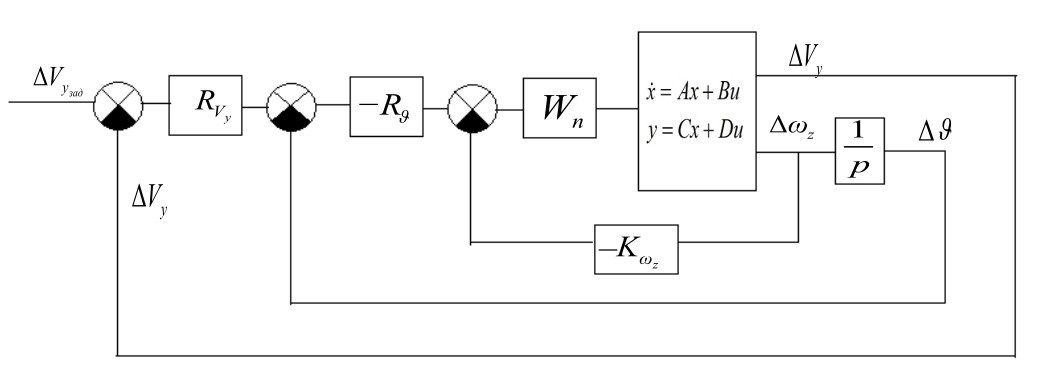
\includegraphics[width=\linewidth]{Оглавление/Part2/Sactions/Content/figures/Схема.jpg}}
    \caption{Структурная схема системы стабилизации вертикальной скорости самолета}
    \label{fig:Схема}
\end{figure}

\subsection{Выбор параметров привода}
    
    При решении задачи синтеза сервопривод описывается передаточной функций колебательного звена:
    
    \begin{equation}
    \label{eq:Привод ограничеия}
        W_{\text{п}}=\frac{1}{T_\text{п}^2p^2+2\xi_\text{п}T_\text{п}p+1}
    \end{equation}
    
    Значение постоянной времени  $T_\text{п}$ сервопривода, от которой зависит его полоса пропускания, определяется следующим образом:
    
    Устанавливается максимальное значение собственной частоты  недемпфированных колебаний $\omega_0=\frac{1}{T_{\text{с}}}$ в варианте управлении продольным движением самолета, и исходя из этих значений, определяется потребная ширина полосы пропускания сервопривода (см. формула \ref{eq:Привод ограничеия}):
    
    \begin{equation}
        \label{eq:Собственная частота привода}
        \omega_\text{п}=10 \omega_{0_{max}}
    \end{equation}
    
    По найденному значению $\omega_\text{п}$ определяется постоянная времени  $T_\text{п}$ как ближайшее к величине $1/ \omega_\text{п}$  значение из ряда чисел: [0,02; 0,025; 0,003; 0,035; 0,04; 0,045; 0,05] (в данном ряде чисел указаны значения постоянной времени, характерные для современных сервоприводов).
    
    \subsubsection{Расчёт $\omega_0$}
    
    Относительный момент тангажа по углу атаки -- 
    \begin{equation}
        \label{eq:Относительный момент тангажа по углу атаки}
        \bar{M}_z^{\alpha} = \frac{m_z^{\alpha}qSb_a}{J_z}
    \end{equation}
    
    Относительная производная подъёмной силы по углу атаки --
    \begin{equation}
        \label{eq:Относительный момент тангажа по угловой скорости тангажа}
        \bar{Y}^\alpha=\frac{C_y^\alpha qS}{mV}
    \end{equation}
    
    Относительный демпфирующий момент тангажа --
    \begin{equation}
        \label{eq:Относительный демпфирующий момент тангажа}
        \bar{M}^{\omega_z}=\frac{m_z^{\omega_z} qS b_a}{J_z}
    \end{equation}
    
    
    Квадрат частоты собственных недемпфированных колебаний --
    \begin{equation}
        \label{eq:Cобственная частота самолёта}
        \omega_0^2=-\bar{Y}^\alpha \bar{M}_z^{\omega_z}-\bar{M}_z^{\alpha}
    \end{equation}
    
    Согласно формулам \ref{eq:Относительный момент тангажа по углу атаки}-\ref{eq:Cобственная частота самолёта} были произведены все необходимые вычисления для каждой узловой точки, результаты вычислений занесены в таблицы \ref{tab:Узловые точки}-\ref{tab:Собственные значения частоты недемпфированных колебаний в узловых точках}


  \begin{longtable}[H]{|c|c|c|c|c|c|c|c|c|c|c|}
    \caption{$\omega_0$ в узловых точках (таб. \ref{tab:Узловые точки})\label{tab:Собственные значения частоты недемпфированных колебаний в узловых точках}}
    \hline 
    $H,$ км &\multicolumn{10}{|c|}{$\omega_0, 1/c$} \\ \hline
    \endfirsthead
    
    \multicolumn{11}{c}%
    {{ \tablename\ \thetable{}: $\omega_0$ в узловых точках}} \\
    \hline 
    $H,$ км &\multicolumn{10}{|c|}{$\omega_0, 1/c$} \\ \hline
    \endhead
    \endfoot
    
    \hline \hline
    \endlastfoot

    0 & 0,88 & 1,21 & 1,54 & 1,87 & 2,24 & 2,64 & 3,13 & 3,78 & 4,66 & 5,74  \\ \hline
    1 & 0,86 & 1,16 & 1,47 & 1,78 & 2,12 & 2,51 & 2,99 & 3,65 & 4,53 & 5,59  \\ \hline
    2 & 0,84 & 1,12 & 1,39 & 1,69 & 2,01 & 2,37 & 2,86 & 3,53 & 4,4 & 5,44  \\ \hline
    3 & 0,81 & 1,07 & 1,32 & 1,6 & 1,9 & 2,25 & 2,74 & 3,41 & 4,28 & 5,3  \\ \hline
    4 & 0,79 & 1,02 & 1,25 & 1,51 & 1,79 & 2,14 & 2,63 & 3,31 & 4,16 & 5,15  \\ \hline
    5 & 0,77 & 0,98 & 1,2 & 1,44 & 1,71 & 2,06 & 2,56 & 3,24 & 4,07 & 5,01  \\ \hline
    6 & 0,75 & 0,94 & 1,15 & 1,37 & 1,63 & 1,98 & 2,49 & 3,17 & 3,98 & 4,87  \\ \hline
    7 & 0,73 & 0,91 & 1,09 & 1,3 & 1,56 & 1,92 & 2,44 & 3,11 & 3,89 & 4,72  \\ \hline
    8 & 0,7 & 0,87 & 1,04 & 1,24 & 1,49 & 1,86 & 2,39 & 3,04 & 3,79 & 4,55  \\ \hline
    9 & 0,69 & 0,84 & 1 & 1,19 & 1,45 & 1,82 & 2,33 & 2,95 & 3,64 & 4,32  \\ \hline
    10 & 0,68 & 0,82 & 0,97 & 1,15 & 1,41 & 1,78 & 2,27 & 2,85 & 3,48 & 4,08  \\ \hline
    11 & 0,67 & 0,79 & 0,93 & 1,11 & 1,37 & 1,75 & 2,22 & 2,75 & 3,32 & 3,85  \\ \hline
    12 & 0,65 & 0,76 & 0,9 & 1,08 & 1,35 & 1,71 & 2,15 & 2,65 & 3,16 & 3,62  \\ \hline
    13 & 0,65 & 0,76 & 0,89 & 1,07 & 1,33 & 1,66 & 2,05 & 2,47 & 2,9 & 3,29  \\ \hline
    14 & 0,66 & 0,76 & 0,9 & 1,08 & 1,33 & 1,62 & 1,95 & 2,3 & 2,66 & 2,99  \\ \hline
    15 & 0,68 & 0,78 & 0,92 & 1,1 & 1,32 & 1,57 & 1,85 & 2,15 & 2,45 & 2,72  \\ \hline
    16 & 0,71 & 0,81 & 0,95 & 1,12 & 1,32 & 1,53 & 1,76 & 2,01 & 2,25 & 2,48  \\ \hline
    17 & 0,82 & 0,92 & 1,04 & 1,16 & 1,3 & 1,45 & 1,6 & 1,76 & 1,92 & 2,08  \\ \hline
    18 & 0,98 & 1,05 & 1,13 & 1,21 & 1,29 & 1,37 & 1,45 & 1,54 & 1,63 & 1,72  \\ \hline
    19  & 1,17 & 1,19 & 1,22 & 1,24 & 1,27 & 1,29 & 1,32 & 1,35 & 1,37 & 1,4 \\ \hline
    \end{longtable}

По данным таблицы \ref{tab:Собственные значения частоты недемпфированных колебаний в узловых точках} можно сделать вывод, что максимальное значение $\omega_0$ находится у поверхности земли со значением $M = 1$ ($\omega_0_{max} = 3.719 \ \frac{1}{c}$).

Используя соотношение (\ref{eq:Собственная частота привода}) получаем, что $\omega_\text{п} = 37,19 \ \frac{1}{c}$ => $T_{\text{п}} = 0.0269 \ c$ 

Из данного ряда чисел [0,02; 0,025; 0,003; 0,035; 0,04; 0,045; 0,05] 0,0269 более близко к 0,025, следовательно, данное число мы и примем за постоянную времени привода. Исходя из вышесказанного, получаем $\omega_\text{п} = 40 \ \frac{1}{c}$ , $T_{\text{п}} = 0.025 \ c, \xi = 0,5$.


    $$W_{\text{п}} = \frac{1}{T_{\text{п}}^2p^2+2\xi_\text{п}T_{\text{п}}p+1} = \frac{1}{0,000156252p^2+0,0125p+1}$$
    
    \begin{center}
        Выводы:
    \end{center}
    
    После выполнения необходимых расчетов преобразований были найдены следующие параметры привода системы стабилизации вертикальной скорости:\\
    $\omega_\text{п} = 40 \ \frac{1}{c}$ \\
    $T_{\text{п}} = 0.025 \ c \\
    \xi = 0,5$\\
    
    Найденные значения параметров соответствуют стандартным значениям для параметров привода и могут быть использованы в последующих частях данной работы. 

    \subsection{Синтез контуров автоматического управления}
    \subsubsection{Выбор коэффициентов обратных связей}
    
    После определения  параметров привода необходимо выбрать рациональные значения коэффициентов обратных связей. Для начала необходимо подобрать коэффициенты $K_\omega_z$ и $K_\vartheta$.
    
    % \subsubsection{Методика расчёта $K_{\vartheta}$}
    
    \subsubsubsection{Методика расчёта  $K_{\omega_z}$ и $K_\vartheta$}
    
    Составим передаточную функцию разомкнутого контура стабилизации угла тангажа
    
    \begin{equation}
    \label{eq:ПФ разомкнутой системы стабилизации тангажа}
        W_{\text{раз} \ \vartheta} = \frac{\Mzf K_{\omega_z}(p+\nu)(T_1_c p+1)}{p(p^2 +2hp+\omega_0^2)(T_{\text{п}}^2p^2+2\xi_\text{п}T_{\text{п}}p+1)},
    \end{equation}
    где $\nu=\frac{K_\vartheta}{K_{\omega_z}}$

    Если выбрано $\nu \approx \frac{1}{T_c}=\omega_0$, то асимптотическая ЛАФЧХ прередаточной функции (\ref{eq:ПФ разомкнутой системы стабилизации тангажа}) имеет 2 участка с наклоном -20 дБ/дек: первый при $\omega < \frac{1}{T_1_c}$, второй  -- при $\frac{1}{T_c}<\omega<\frac{1}{T_\text{п}}$. Для интересующей нас второй асимптоты ЛАФЧХ с наклоном -20 дБ/дек на основе (\ref{eq:ПФ разомкнутой системы стабилизации тангажа}) получим следующую формулу:
    
    \begin{equation}
    \label{eq:ПФ разомкнутой системы стабилизации тангажа 2}
        W_{\text{раз} \ \vartheta} = \frac{K_{\omega_z} T_1_c}{T_c^2p}=-\frac{K_{\omega_z} \Mzf}{p}, \frac{1}{T_c} < \omega < \frac{1}{T_{\text{п}}}.
    \end{equation}
    
    Частота среза частотной характеристики передаточной функции (\ref{eq:ПФ разомкнутой системы стабилизации тангажа 2}) $\omega_{cp} = K_{\omega_z}\Mzf.$ Так как фазовая частотная характеристика передаточной функции (\ref{eq:ПФ разомкнутой системы стабилизации тангажа}) достигает значения $-\pi$ на частоте $\omega_{-\pi} \approx \frac{1}{T_\text{п}}$, то для граничного значения $K_{\omega_z}$ (при котором $\omega_{cp} = \omega_{-\pi}$) имеем 
    
    \begin{equation}
        K_{\omega_z_{\text{гр}}} = \frac{1}{|\Mzf|T_\text{п}}.
    \end{equation}
    
    Исходя из запаса по амплитуде 12 дБ/дек можно принять 
    \begin{equation}
        \label{eq:K_wz}
        K_{\omega_z} = 0,25K_{\omega_z_{\text{гр}}}, \ \ \frac{K_{\vartheta}}{K_{\omega_z}} < \frac{0,25}{T_\text{п}}.
    \end{equation}

    \subsubsubsection{Результаты расчётов $K_{\omega_z}$ и $K_\vartheta$}
    
    \begin{longtable}[H]{|c|c|c|c|c|c|c|c|c|c|c|}
    \caption{Результаты расчётов $K_{\omega_z}, c$ в узловых точках (таб. \ref{tab:Узловые точки})}
    \hline 
    $H,$ км &\multicolumn{10}{|c|}{$K_{\omega_z}, c$} \\ \hline
    \endfirsthead
    
    \multicolumn{11}{c}%
    {{ \tablename\ \thetable{}: Результаты расчётов $K_{\omega_z}, c$ в узловых точках}} \\
    \hline 
    $H,$ км &\multicolumn{10}{|c|}{$K_{\omega_z}, c$} \\ \hline
    \endhead
    \endfoot
    
    \hline \hline
    \endlastfoot

    \hline
    0 & 6,11 & 3,24 & 1,98 & 1,3 & 0,9 & 0,67 & 0,51 & 0,36 & 0,23 & 0,15  \\ \hline
    1 & 6,01 & 3,29 & 2,04 & 1,35 & 0,95 & 0,71 & 0,53 & 0,37 & 0,23 & 0,15  \\ \hline
    2 & 5,98 & 3,37 & 2,12 & 1,41 & 1 & 0,76 & 0,56 & 0,38 & 0,24 & 0,16  \\ \hline
    3 & 6,02 & 3,47 & 2,21 & 1,49 & 1,07 & 0,81 & 0,59 & 0,39 & 0,25 & 0,17  \\ \hline
    4 & 6,11 & 3,6 & 2,31 & 1,57 & 1,15 & 0,87 & 0,62 & 0,4 & 0,25 & 0,17  \\ \hline
    5 & 6 & 3,64 & 2,37 & 1,64 & 1,22 & 0,91 & 0,63 & 0,4 & 0,26 & 0,18  \\ \hline
    6 & 5,98 & 3,71 & 2,46 & 1,73 & 1,3 & 0,96 & 0,65 & 0,41 & 0,27 & 0,19  \\ \hline
    7 & 6,01 & 3,81 & 2,56 & 1,83 & 1,39 & 1,01 & 0,66 & 0,42 & 0,28 & 0,21  \\ \hline
    8 & 6,11 & 3,94 & 2,69 & 1,96 & 1,49 & 1,06 & 0,68 & 0,43 & 0,3 & 0,22  \\ \hline
    9 & 5,93 & 3,94 & 2,77 & 2,08 & 1,57 & 1,09 & 0,7 & 0,46 & 0,32 & 0,25  \\ \hline
    10 & 5,82 & 3,99 & 2,9 & 2,22 & 1,66 & 1,13 & 0,73 & 0,49 & 0,35 & 0,28  \\ \hline
    11 & 5,79 & 4,09 & 3,07 & 2,37 & 1,74 & 1,16 & 0,76 & 0,53 & 0,39 & 0,31  \\ \hline
    12 & 5,82 & 4,24 & 3,27 & 2,52 & 1,81 & 1,2 & 0,81 & 0,57 & 0,43 & 0,35  \\ \hline
    13 & 5,44 & 4,22 & 3,36 & 2,59 & 1,85 & 1,27 & 0,89 & 0,65 & 0,51 & 0,42  \\ \hline
    14 & 5,23 & 4,26 & 3,42 & 2,62 & 1,89 & 1,34 & 0,98 & 0,75 & 0,6 & 0,5  \\ \hline
    15 & 5,15 & 4,26 & 3,42 & 2,6 & 1,92 & 1,42 & 1,08 & 0,86 & 0,7 & 0,6  \\ \hline
    16 & 5,05 & 4,17 & 3,32 & 2,55 & 1,95 & 1,51 & 1,2 & 0,98 & 0,82 & 0,71  \\ \hline
    17 & 4,27 & 3,58 & 2,96 & 2,44 & 2,02 & 1,69 & 1,44 & 1,24 & 1,08 & 0,96  \\ \hline
    18 & 3,3 & 2,94 & 2,62 & 2,35 & 2,11 & 1,9 & 1,72 & 1,57 & 1,44 & 1,33  \\ \hline
    19  & 2,53 & 2,44 & 2,36 & 2,28 & 2,2 & 2,13 & 2,06 & 2 & 1,94 & 1,88 \\ \hline
    \end{longtable}

    \begin{longtable}[H]{|c|c|c|c|c|c|c|c|c|c|c|}
    \caption{Результаты расчётов $K_{\vartheta}$ в узловых точках (таб. \ref{tab:Узловые точки})}
    \hline 
    $H,$ км &\multicolumn{10}{|c|}{$K_{\vartheta}$ } \\ \hline
    \endfirsthead
    
    \multicolumn{11}{c}%
    {{ \tablename\ \thetable{}: Результаты расчётов $K_{\vartheta}$ в узловых точках}} \\
    \hline 
    $H,$ км &\multicolumn{10}{|c|}{$K_{\vartheta}$ } \\ \hline
    \endhead
    \endfoot
    
    \hline \hline
    \endlastfoot

    0 & 2,82 & 1,79 & 1,29 & 0,97 & 0,76 & 0,63 & 0,53 & 0,41 & 0,29 & 0,21  \\ \hline
    1 & 2,71 & 1,75 & 1,27 & 0,96 & 0,76 & 0,63 & 0,52 & 0,4 & 0,28 & 0,21  \\ \hline
    2 & 2,58 & 1,72 & 1,25 & 0,95 & 0,75 & 0,63 & 0,51 & 0,38 & 0,27 & 0,2  \\ \hline
    3 & 2,54 & 1,71 & 1,24 & 0,94 & 0,76 & 0,63 & 0,5 & 0,36 & 0,26 & 0,2  \\ \hline
    4 & 2,51 & 1,7 & 1,23 & 0,95 & 0,76 & 0,63 & 0,49 & 0,35 & 0,25 & 0,19  \\ \hline
    5 & 2,41 & 1,64 & 1,21 & 0,94 & 0,77 & 0,62 & 0,48 & 0,33 & 0,24 & 0,19  \\ \hline
    6 & 2,34 & 1,64 & 1,21 & 0,93 & 0,77 & 0,62 & 0,45 & 0,32 & 0,23 & 0,19  \\ \hline
    7 & 2,29 & 1,6 & 1,18 & 0,94 & 0,77 & 0,61 & 0,43 & 0,3 & 0,23 & 0,19  \\ \hline
    8 & 2,21 & 1,58 & 1,19 & 0,95 & 0,78 & 0,59 & 0,41 & 0,29 & 0,22 & 0,19  \\ \hline
    9 & 2,14 & 1,54 & 1,17 & 0,96 & 0,77 & 0,58 & 0,4 & 0,29 & 0,23 & 0,19  \\ \hline
    10 & 2,04 & 1,48 & 1,16 & 0,96 & 0,77 & 0,55 & 0,39 & 0,29 & 0,23 & 0,2  \\ \hline
    11 & 1,98 & 1,48 & 1,2 & 0,98 & 0,75 & 0,54 & 0,38 & 0,29 & 0,24 & 0,21  \\ \hline
    12 & 1,87 & 1,45 & 1,18 & 0,99 & 0,74 & 0,52 & 0,37 & 0,29 & 0,24 & 0,21  \\ \hline
    13 & 1,75 & 1,4 & 1,18 & 0,96 & 0,71 & 0,51 & 0,38 & 0,3 & 0,26 & 0,23  \\ \hline
    14 & 1,63 & 1,37 & 1,13 & 0,92 & 0,68 & 0,51 & 0,39 & 0,32 & 0,28 & 0,25  \\ \hline
    15 & 1,55 & 1,33 & 1,1 & 0,86 & 0,66 & 0,51 & 0,4 & 0,34 & 0,3 & 0,26  \\ \hline
    16 & 1,47 & 1,26 & 1,03 & 0,82 & 0,65 & 0,52 & 0,42 & 0,36 & 0,31 & 0,29  \\ \hline
    17 & 1,24 & 1,04 & 0,89 & 0,76 & 0,63 & 0,54 & 0,48 & 0,42 & 0,38 & 0,35  \\ \hline
    18 & 0,96 & 0,86 & 0,76 & 0,68 & 0,63 & 0,57 & 0,54 & 0,49 & 0,46 & 0,43  \\ \hline
    19  & 0,71 & 0,69 & 0,66 & 0,66 & 0,64 & 0,62 & 0,6 & 0,58 & 0,56 & 0,55 \\ \hline
    \end{longtable}
 
    \begin{longtable}[H]{|c|c|c|c|c|c|c|c|c|c|c|}
    \caption[Результаты расчётов $q \cdot 10^{-3}$,1/м в узловых точках]{Результаты расчётов $q \cdot 10^{-3}$,1/м в узловых точках \label{tab:Результаты расчётов $q(H,M),$Н/м$^2$} \\
    \hline 
    $H,$ км &\multicolumn{10}{|c|}{$q(H,M) \cdot 10^{-3},$Н/м$^2$ }\\ \hline
    \endfirsthead
    
    \multicolumn{11}{c}%
    {{ \tablename\ \thetable{}: Результаты расчётов $q \cdot 10^{-3}$,1/м в узловых точках}} \\
    \hline 
    $H,$ км &\multicolumn{10}{|c|}{$q(H,M) \cdot 10^{-3},$Н/м$^2$ }\\ \hline
    \endhead
    \endfoot
    
    \hline \hline
    \endlastfoot

        0 & 5403 & 10278 & 16707 & 24690 & 34227 & 45318 & 57963 & 72162 & 87915 & 105223  \\ \hline
        1 & 5503 & 10114 & 16117 & 23513 & 32301 & 42481 & 54054 & 67019 & 81376 & 97126  \\ \hline
        2 & 5540 & 9874 & 15453 & 22275 & 30342 & 39653 & 50207 & 62006 & 75049 & 89336  \\ \hline
        3 & 5517 & 9568 & 14727 & 20994 & 28370 & 36854 & 46446 & 57147 & 68955 & 81872  \\ \hline
        4 & 5440 & 9204 & 13952 & 19685 & 26402 & 34104 & 42789 & 52459 & 63113 & 74751  \\ \hline
        5 & 5543 & 9063 & 13445 & 18689 & 24794 & 31760 & 39588 & 48277 & 57827 & 68239  \\ \hline
        6 & 5570 & 8838 & 12858 & 17630 & 23152 & 29426 & 36452 & 44228 & 52757 & 62036  \\ \hline
        7 & 5526 & 8540 & 12206 & 16525 & 21497 & 27123 & 33401 & 40333 & 47917 & 56155  \\ \hline
        8 & 5419 & 8178 & 11502 & 15392 & 19847 & 24867 & 30454 & 36605 & 43323 & 50605  \\ \hline
        9 & 5548 & 8053 & 11025 & 14462 & 18365 & 22733 & 27567 & 32867 & 38632 & 44863  \\ \hline
        10 & 5581 & 7835 & 10470 & 13487 & 16885 & 20664 & 24825 & 29367 & 34290 & 39595  \\ \hline
        11 & 5527 & 7535 & 9854 & 12483 & 15423 & 18673 & 22235 & 26106 & 30289 & 34782  \\ \hline
        12 & 5407 & 7184 & 9213 & 11494 & 14027 & 16812 & 19849 & 23138 & 26679 & 30473  \\ \hline
        13 & 5646 & 7158 & 8848 & 10718 & 12767 & 14995 & 17402 & 19988 & 22753 & 25697  \\ \hline
        14 & 5790 & 7055 & 8444 & 9959 & 11598 & 13363 & 15252 & 17266 & 19405 & 21668  \\ \hline
        15 & 5848 & 6888 & 8013 & 9223 & 10518 & 11899 & 13364 & 14915 & 16550 & 18271  \\ \hline
        16 & 5831 & 6670 & 7564 & 8516 & 9523 & 10587 & 11707 & 12883 & 14116 & 15405  \\ \hline
        17 & 6162 & 6723 & 7310 & 7921 & 8556 & 9216 & 9901 & 10610 & 11344 & 12102  \\ \hline
        18 & 6380 & 6694 & 7014 & 7343 & 7679 & 8022 & 8373 & 8732 & 9098 & 9472  \\ \hline
        19  & 6497 & 6593 & 6689 & 6786 & 6884 & 6982 & 7082 & 7182 & 7282 & 7383 \\ \hline
    \end{longtable}
    
    \begin{figure}[H]
        \center{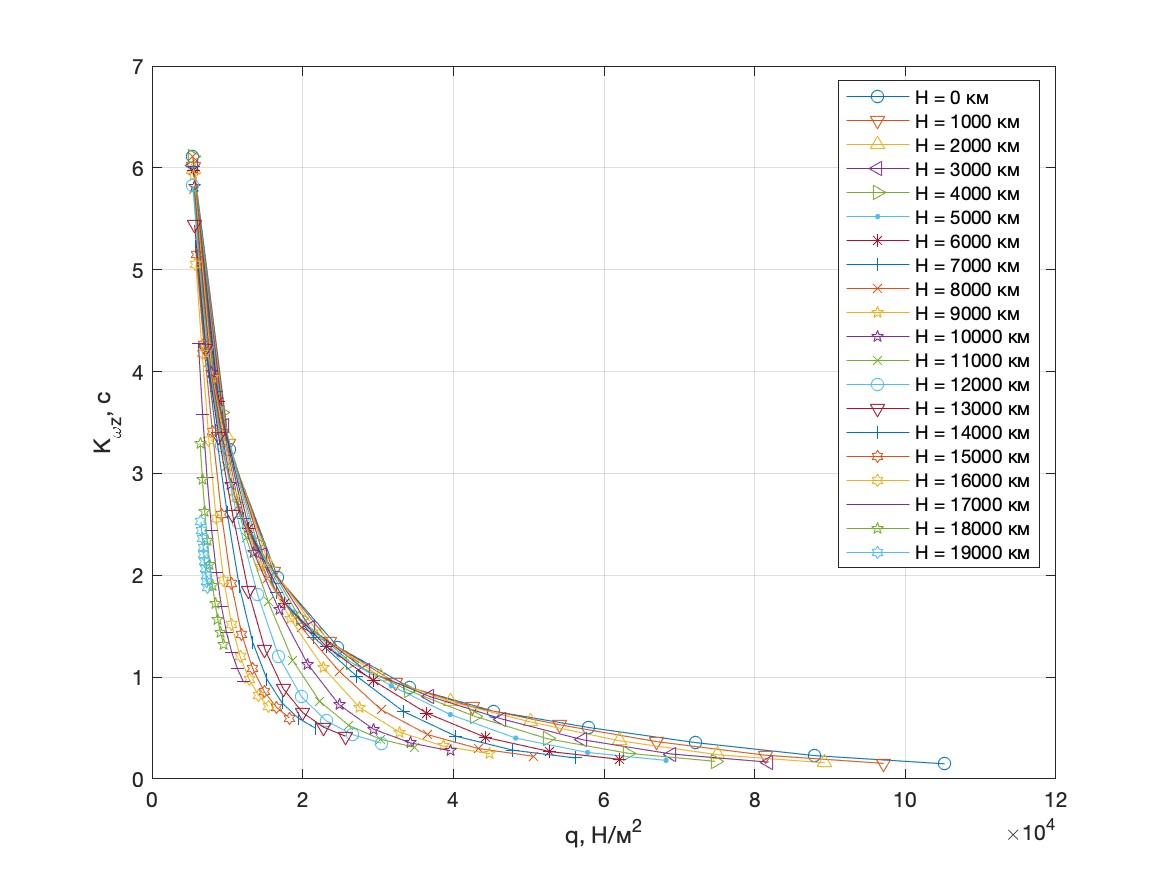
\includegraphics[width=\linewidth]{Оглавление/Part2/Sactions/Content/figures/K_wz.jpg}}
        \caption{$K_{\omega_z}(q), $с}
        \label{fig:K_wz}
    \end{figure}
    
    \begin{figure}[H]
        \center{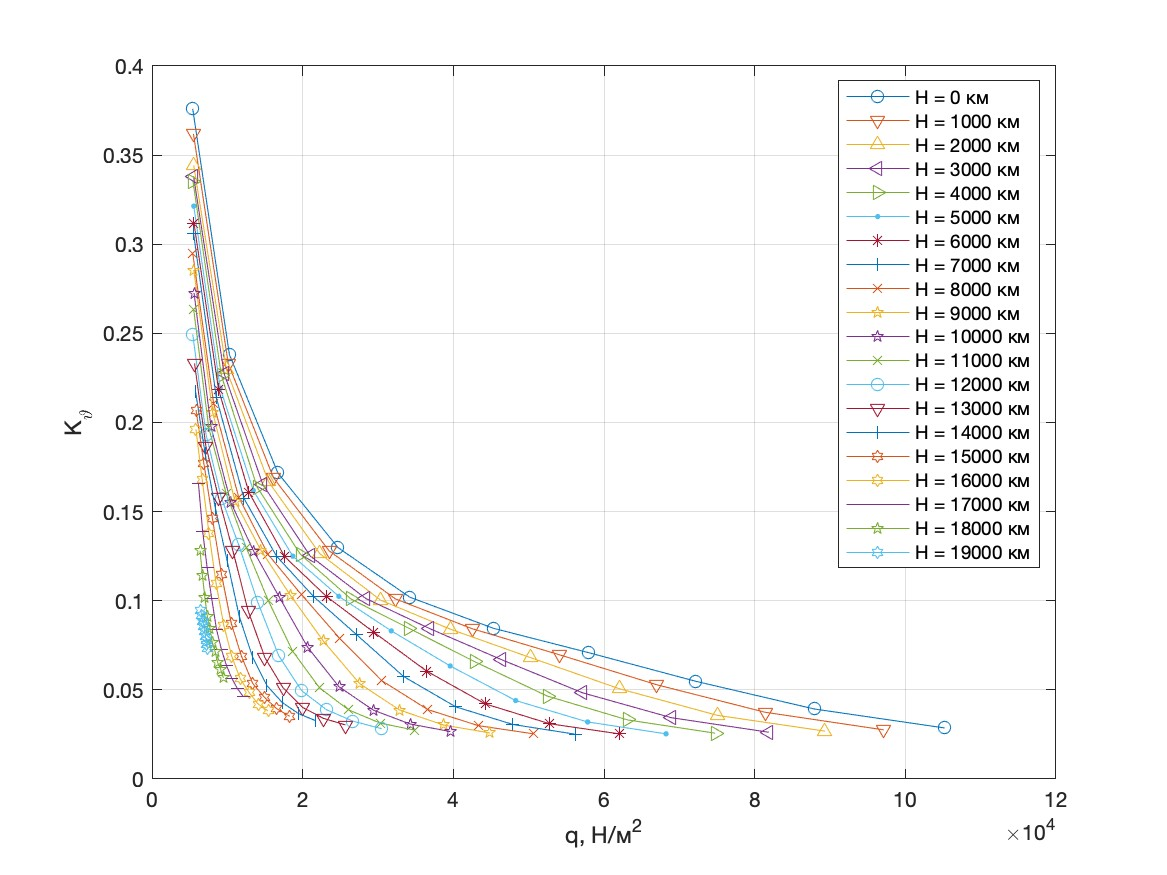
\includegraphics[width=\linewidth]{Оглавление/Part2/Sactions/Content/figures/K_v.jpg}}
        \caption{$K_{\vartheta}(q) $}
        \label{fig:K_wz}
    \end{figure}
    
    \subsubsection{Расчёты параметров для PI-контроллера}
    
    Передаточнвая функция разомкнутой системы стабилизации вертикальной скорости имеет вид:
    \begin{equation}
    \label{eq:ПФ разомкнутой системы стабилизации Vy}
        W^{V_y}_\text{раз}=R_H(p)\frac{K_H}{(\tau_1p+1)(\tau_2^2p^2+2\xi_2\tau_2p+1)}
    \end{equation}
    
    Из выражения (\ref{eq:ПФ разомкнутой системы стабилизации Vy}) следует, что система имеет собственную статическую ошибку. Устранение статической ошибки может быть достигнуто введением интеграла в закон управления. При этом передаточная функция регулятора принимает вид
    \begin{equation}
        \label{eq:PI-контроллер}
        R_{V_y}(p) = i_H + i_p\frac{1}{p}
    \end{equation}
    
    \subsubsubsection{Методика расчёта $i_H$ и $i_p$}
    
    Составим передаточную функцию учитывая соотношение (\ref{eq:PI-контроллер}) получим
    \begin{equation}
        \label{eq:ПФ с PI}
        W_\text{раз}^{V_{y}} = \frac{K_H (i_H+i_p\frac{1}{p})}{(\tau_1p+1)(\tau_2^2p^2+2\xi_2\tau_2p+1)}
    \end{equation}
    
    Преобразуем передаточную функцию (\ref{eq:ПФ с PI})
    
    \begin{equation}
        \label{eq:ПФ + PI преобразованная}
        W_\text{раз}^{V_y} = \frac{K_H i_p (\frac{i_H}{i_p}p + 1)}{p(\tau_1p+1)(\tau_2^2p^2+2\xi_2\tau_2p+1)}
    \end{equation}
    
    Из передаточной функции (\ref{eq:ПФ + PI преобразованная}) видно, что $\omega_{cp} \approx K_H i_p$. Делаем вывод, что 
    
    \begin{equation}
    \label{eq:i_p}
        i_p = 0,25 \frac{1}{\tau_1 K_H}
    \end{equation}
    
    Для уменьшения времени регулирования приравняем $\frac{i_H}{i_p} = \tau_1$
    
    \begin{equation}
        \label{eq:i_H}
        i_H = i_p \cdot \tau_1
    \end{equation}
    
    Подробнее об этом можно найти в учебнике \cite{UDLA}
    
    \begin{longtable}[H]{|c|c|c|c|c|c|c|c|c|c|c|}
    \caption[Результаты расчётов $i_p \cdot 10^{3}$,1/м в узловых точках]{Результаты расчётов $i_p \cdot 10^{3}$,1/м в узловых точках \label{tab:Результаты расчётов $i_p(H,M),$Н/м$^2$} \\
    \hline 
    $H,$ км &\multicolumn{10}{|c|}{$i_p \cdot 10^{3}$, 1/м } \\ \hline
    \endfirsthead
    
    \multicolumn{11}{c}%
    {{ \tablename\ \thetable{}: Результаты расчётов $i_p \cdot 10^{3}$,1/м в узловых точках}} \\
    \hline 
    $H,$ км &\multicolumn{10}{|c|}{$i_p \cdot 10^{3}$, 1/м } \\ \hline
    \endhead
    \endfoot
    
    \hline \hline
    \endlastfoot

    0 & 3,75 & 2,48 & 1,88 & 1,52 & 1,29 & 1,14 & 1,05 & 1,04 & 1,1 & 1,2  \\ \hline
    1 & 3,63 & 2,44 & 1,87 & 1,52 & 1,3 & 1,15 & 1,08 & 1,09 & 1,16 & 1,26  \\ \hline
    2 & 3,48 & 2,42 & 1,87 & 1,52 & 1,3 & 1,17 & 1,11 & 1,14 & 1,22 & 1,33  \\ \hline
    3 & 3,43 & 2,41 & 1,86 & 1,53 & 1,32 & 1,19 & 1,15 & 1,19 & 1,29 & 1,41  \\ \hline
    4 & 3,41 & 2,41 & 1,87 & 1,55 & 1,34 & 1,22 & 1,2 & 1,25 & 1,36 & 1,48  \\ \hline
    5 & 3,3 & 2,37 & 1,87 & 1,56 & 1,36 & 1,25 & 1,25 & 1,32 & 1,43 & 1,55  \\ \hline
    6 & 3,22 & 2,37 & 1,88 & 1,57 & 1,38 & 1,3 & 1,31 & 1,4 & 1,51 & 1,63  \\ \hline
    7 & 3,18 & 2,36 & 1,87 & 1,59 & 1,41 & 1,35 & 1,38 & 1,47 & 1,59 & 1,7  \\ \hline
    8 & 3,1 & 2,35 & 1,9 & 1,62 & 1,46 & 1,4 & 1,45 & 1,55 & 1,66 & 1,77  \\ \hline
    9 & 3,04 & 2,33 & 1,9 & 1,65 & 1,5 & 1,48 & 1,54 & 1,64 & 1,74 & 1,82  \\ \hline
    10 & 2,95 & 2,29 & 1,91 & 1,68 & 1,56 & 1,55 & 1,62 & 1,72 & 1,81 & 1,88  \\ \hline
    11 & 2,91 & 2,32 & 1,98 & 1,74 & 1,63 & 1,64 & 1,72 & 1,81 & 1,88 & 1,93  \\ \hline
    12 & 2,82 & 2,31 & 1,98 & 1,82 & 1,73 & 1,73 & 1,8 & 1,89 & 1,95 & 1,98  \\ \hline
    13 & 2,71 & 2,27 & 2,03 & 1,89 & 1,81 & 1,83 & 1,89 & 1,94 & 2 & 2,03  \\ \hline
    14 & 2,59 & 2,26 & 2,05 & 1,96 & 1,91 & 1,94 & 1,97 & 2,03 & 2,06 & 2,08  \\ \hline
    15 & 2,52 & 2,29 & 2,13 & 2,05 & 2,02 & 2,05 & 2,06 & 2,11 & 2,12 & 2,13  \\ \hline
    16 & 2,49 & 2,34 & 2,24 & 2,19 & 2,17 & 2,17 & 2,16 & 2,19 & 2,18 & 2,19  \\ \hline
    17 & 2,47 & 2,37 & 2,34 & 2,33 & 2,28 & 2,29 & 2,29 & 2,29 & 2,28 & 2,28  \\ \hline
    18 & 2,54 & 2,5 & 2,45 & 2,42 & 2,44 & 2,41 & 2,42 & 2,39 & 2,4 & 2,38  \\ \hline
    19  & 2,59 & 2,58 & 2,56 & 2,61 & 2,59 & 2,58 & 2,57 & 2,55 & 2,54 & 2,53 \\ \hline
    \end{longtable}

        
  \begin{longtable}[H]{|c|c|c|c|c|c|c|c|c|c|c|}
    \caption[Результаты расчётов $i_H \cdot 10^{3}$,1/м в узловых точках]{Результаты расчётов $i_H \cdot 10^{3}$,1/м в узловых точках \label{tab:Результаты расчётов $i_H(H,M),$Н/м$^2$} \\
    \hline 
    $H,$ км &\multicolumn{10}{|c|}{$i_H \cdot 10^{3}$, 1/м } \\ \hline
    \endfirsthead
    
    \multicolumn{11}{c}%
    {{ \tablename\ \thetable{}: Результаты расчётов $i_H \cdot 10^{3}$,1/м в узловых точках}} \\
    \hline 
    $H,$ км &\multicolumn{10}{|c|}{$i_H \cdot 10^{3}$, 1/м } \\ \hline
    \endhead
    \endfoot
    
    \hline \hline
    \endlastfoot

    0 & 0,99 & 0,89 & 0,86 & 0,84 & 0,84 & 0,86 & 0,9 & 1 & 1,19 & 1,49  \\ \hline
    1 & 0,92 & 0,83 & 0,8 & 0,78 & 0,79 & 0,8 & 0,85 & 0,96 & 1,16 & 1,46  \\ \hline
    2 & 0,84 & 0,77 & 0,74 & 0,73 & 0,73 & 0,75 & 0,8 & 0,92 & 1,13 & 1,43  \\ \hline
    3 & 0,78 & 0,72 & 0,69 & 0,67 & 0,68 & 0,7 & 0,76 & 0,89 & 1,1 & 1,4  \\ \hline
    4 & 0,73 & 0,67 & 0,64 & 0,63 & 0,63 & 0,65 & 0,72 & 0,86 & 1,06 & 1,36  \\ \hline
    5 & 0,68 & 0,61 & 0,59 & 0,58 & 0,59 & 0,61 & 0,69 & 0,83 & 1,04 & 1,32  \\ \hline
    6 & 0,62 & 0,58 & 0,55 & 0,54 & 0,55 & 0,58 & 0,66 & 0,8 & 1,01 & 1,28  \\ \hline
    7 & 0,58 & 0,53 & 0,51 & 0,5 & 0,51 & 0,55 & 0,63 & 0,77 & 0,97 & 1,22  \\ \hline
    8 & 0,53 & 0,49 & 0,47 & 0,46 & 0,48 & 0,52 & 0,61 & 0,74 & 0,93 & 1,16  \\ \hline
    9 & 0,49 & 0,46 & 0,44 & 0,43 & 0,45 & 0,49 & 0,58 & 0,71 & 0,88 & 1,07  \\ \hline
    10 & 0,45 & 0,42 & 0,4 & 0,4 & 0,42 & 0,47 & 0,55 & 0,68 & 0,83 & 0,99  \\ \hline
    11 & 0,42 & 0,39 & 0,38 & 0,38 & 0,39 & 0,44 & 0,53 & 0,64 & 0,77 & 0,91  \\ \hline
    12 & 0,37 & 0,35 & 0,34 & 0,35 & 0,37 & 0,41 & 0,49 & 0,59 & 0,71 & 0,81  \\ \hline
    13 & 0,34 & 0,32 & 0,31 & 0,32 & 0,34 & 0,38 & 0,45 & 0,52 & 0,62 & 0,7  \\ \hline
    14 & 0,3 & 0,29 & 0,29 & 0,3 & 0,32 & 0,36 & 0,41 & 0,47 & 0,54 & 0,61  \\ \hline
    15 & 0,27 & 0,27 & 0,27 & 0,28 & 0,3 & 0,34 & 0,37 & 0,43 & 0,48 & 0,53  \\ \hline
    16 & 0,25 & 0,25 & 0,26 & 0,27 & 0,29 & 0,31 & 0,34 & 0,38 & 0,42 & 0,46  \\ \hline
    17 & 0,24 & 0,24 & 0,25 & 0,26 & 0,27 & 0,29 & 0,31 & 0,33 & 0,35 & 0,37  \\ \hline
    18 & 0,23 & 0,24 & 0,24 & 0,25 & 0,26 & 0,26 & 0,27 & 0,28 & 0,3 & 0,3  \\ \hline
    19  & 0,23 & 0,23 & 0,23 & 0,24 & 0,24 & 0,24 & 0,25 & 0,25 & 0,25 & 0,25 \\ \hline
    \end{longtable}


\begin{figure}[H]
        \center{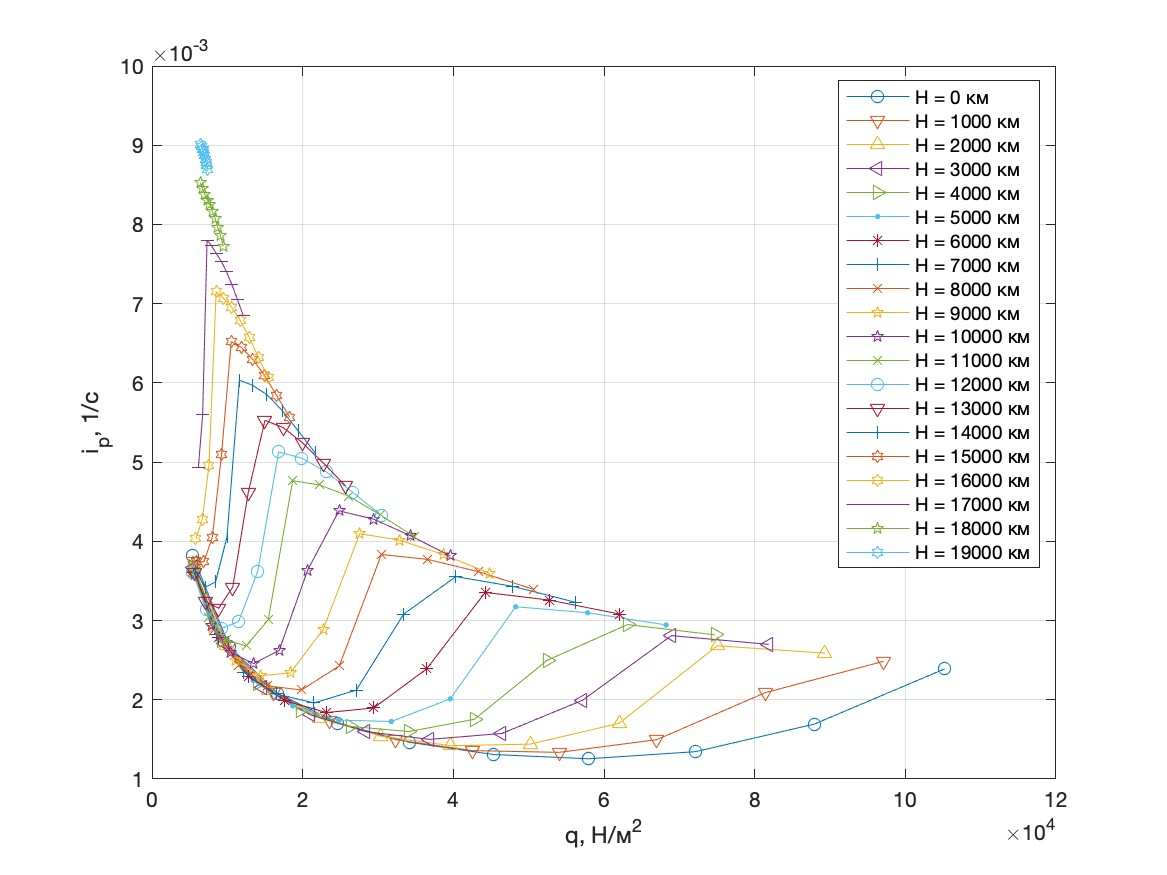
\includegraphics[width=\linewidth]{Оглавление/Part2/Sactions/Content/figures/i_p.jpg}}
        \caption{$i_p(q), $1/м}
        \label{fig:i_p}
    \end{figure} 

\begin{figure}[H]
        \center{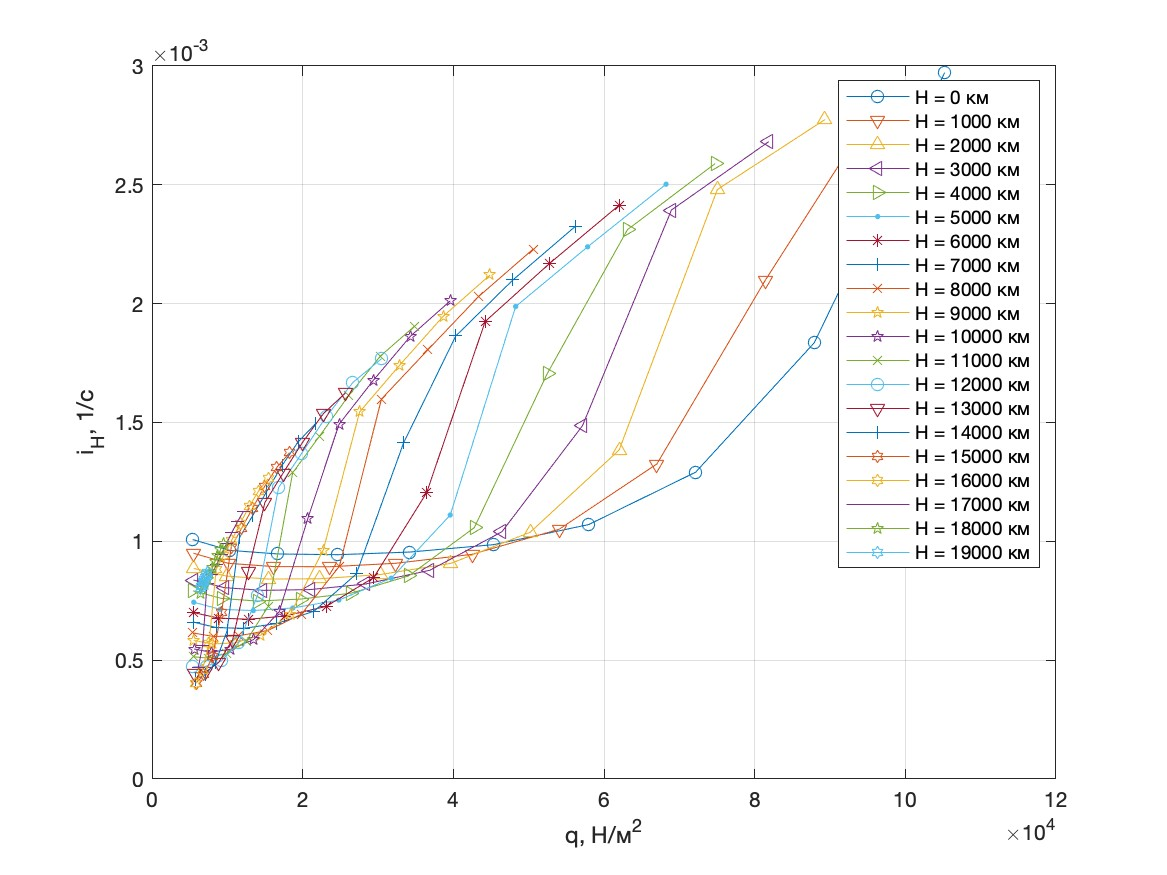
\includegraphics[width=\linewidth]{Оглавление/Part2/Sactions/Content/figures/i_H.jpg}}
        \caption{$i_H(q), $1/м}
        \label{fig:i_H}
    \end{figure} 
    

Для выполнения частотного анализа, который производится в следующем подразделе, необходимо по вышеприведенным графикам и таблицам определить коэффициенты обратных связей при минимальной скоростном напоре, максимальном скоростном напоре и скоростном напоре крейсерского полета. Значения найденных коэффициентов оформлены в виде таблиц \ref{tab:q_min} - \ref{tab:q_kr}


\begin{table}[H]
    \centering
    \caption{Коэффициенты обратных связей, соответствующие $q_{min}$}
    \begin{tabular}{|c|c|c|c|c|c|c|c|}
    \hline
        $H,$ км & $M$ & $q, H / \text{м}^2$ & $K_{\omega_z}, c$ & $K_\vartheta$ & $K_H,$м/c &$i_H$&$i_p$\\ \hline
        0& 0,2760& 5403  &5,31 & 30,472&156,1 &7,8$\cdot 10^{-2}$&1,14 $\cdot 10^{-2}$\\ \hline
    \end{tabular}
    \label{tab:q_min}
\end{table}

\begin{table}[H]
    \centering
    \caption{Коэффициенты обратных связей, соответствующие $q_{max}$}
    \begin{tabular}{|c|c|c|c|c|c|c|c|}
    \hline
        $H,$ км & $M$ & $q, H / \text{м}^2$ & $K_{\omega_z}, c$ & $K_\vartheta$ & $K_H,$м/c &$i_H$&$i_p$ \\ \hline
        0& 1,0976 &105220& 0,3545 & 2,035&340,4&3,6 $\cdot 10^{-3}$&3,4 $\cdot 10^{-3}$\\ \hline
    \end{tabular}
    \label{tab:q_max}
\end{table}


\begin{table}[H]
    \centering
    \caption{Коэффициенты обратных связей, соответствующие $q_\text{кр}$}
    \begin{tabular}{|c|c|c|c|c|c|c|c|}
    \hline
        $H,$ км & $M$ & $q, H / \text{м}^2$ & $K_{\omega_z}, c$ & $K_\vartheta$ & $K_H,$м/c &$i_H$&$i_p$ \\ \hline
        17&0,928&5438 &3,157 & 1,1 &222,0199 &2,8 $\cdot 10^{-3}$&4,4 $\cdot 10^{-4}$\\ \hline
    \end{tabular}
    \label{tab:q_kr}
\end{table}

\begin{center}
    Выводы:
\end{center}

Полученные значения коэффициентов обратных связей были успешно найдены и применены на модели рассматриваемой системы стабилизации вертикальной скорости в системе «Simulink». Моделирование показало, что коэффициенты найдены верно, так как заданная вертикальная скорость равена вертикальной скорости на выходе из системы. Более подробно будут показаны результаты моделирования и сама модель в разделе «Нелинейное моделирование» (раздел 3).

\subsubsection{Частотный анализ}

Целью частотного анализа является построение логарифмических амплитудных и фазовых частотных характеристик (ЛАФЧХ) разомкнутых и замкнутых контуров управления до синтеза и после синтеза и проведение их сравнительного анализа.
% ________________________________________________________________________________________________
\subsubsubsection{Частотный анализ $q_{min}$}

\begin{center}
    Контур демпфирования угловой скорости тангажа:
\end{center}

\begin{figure}[H]
    \center{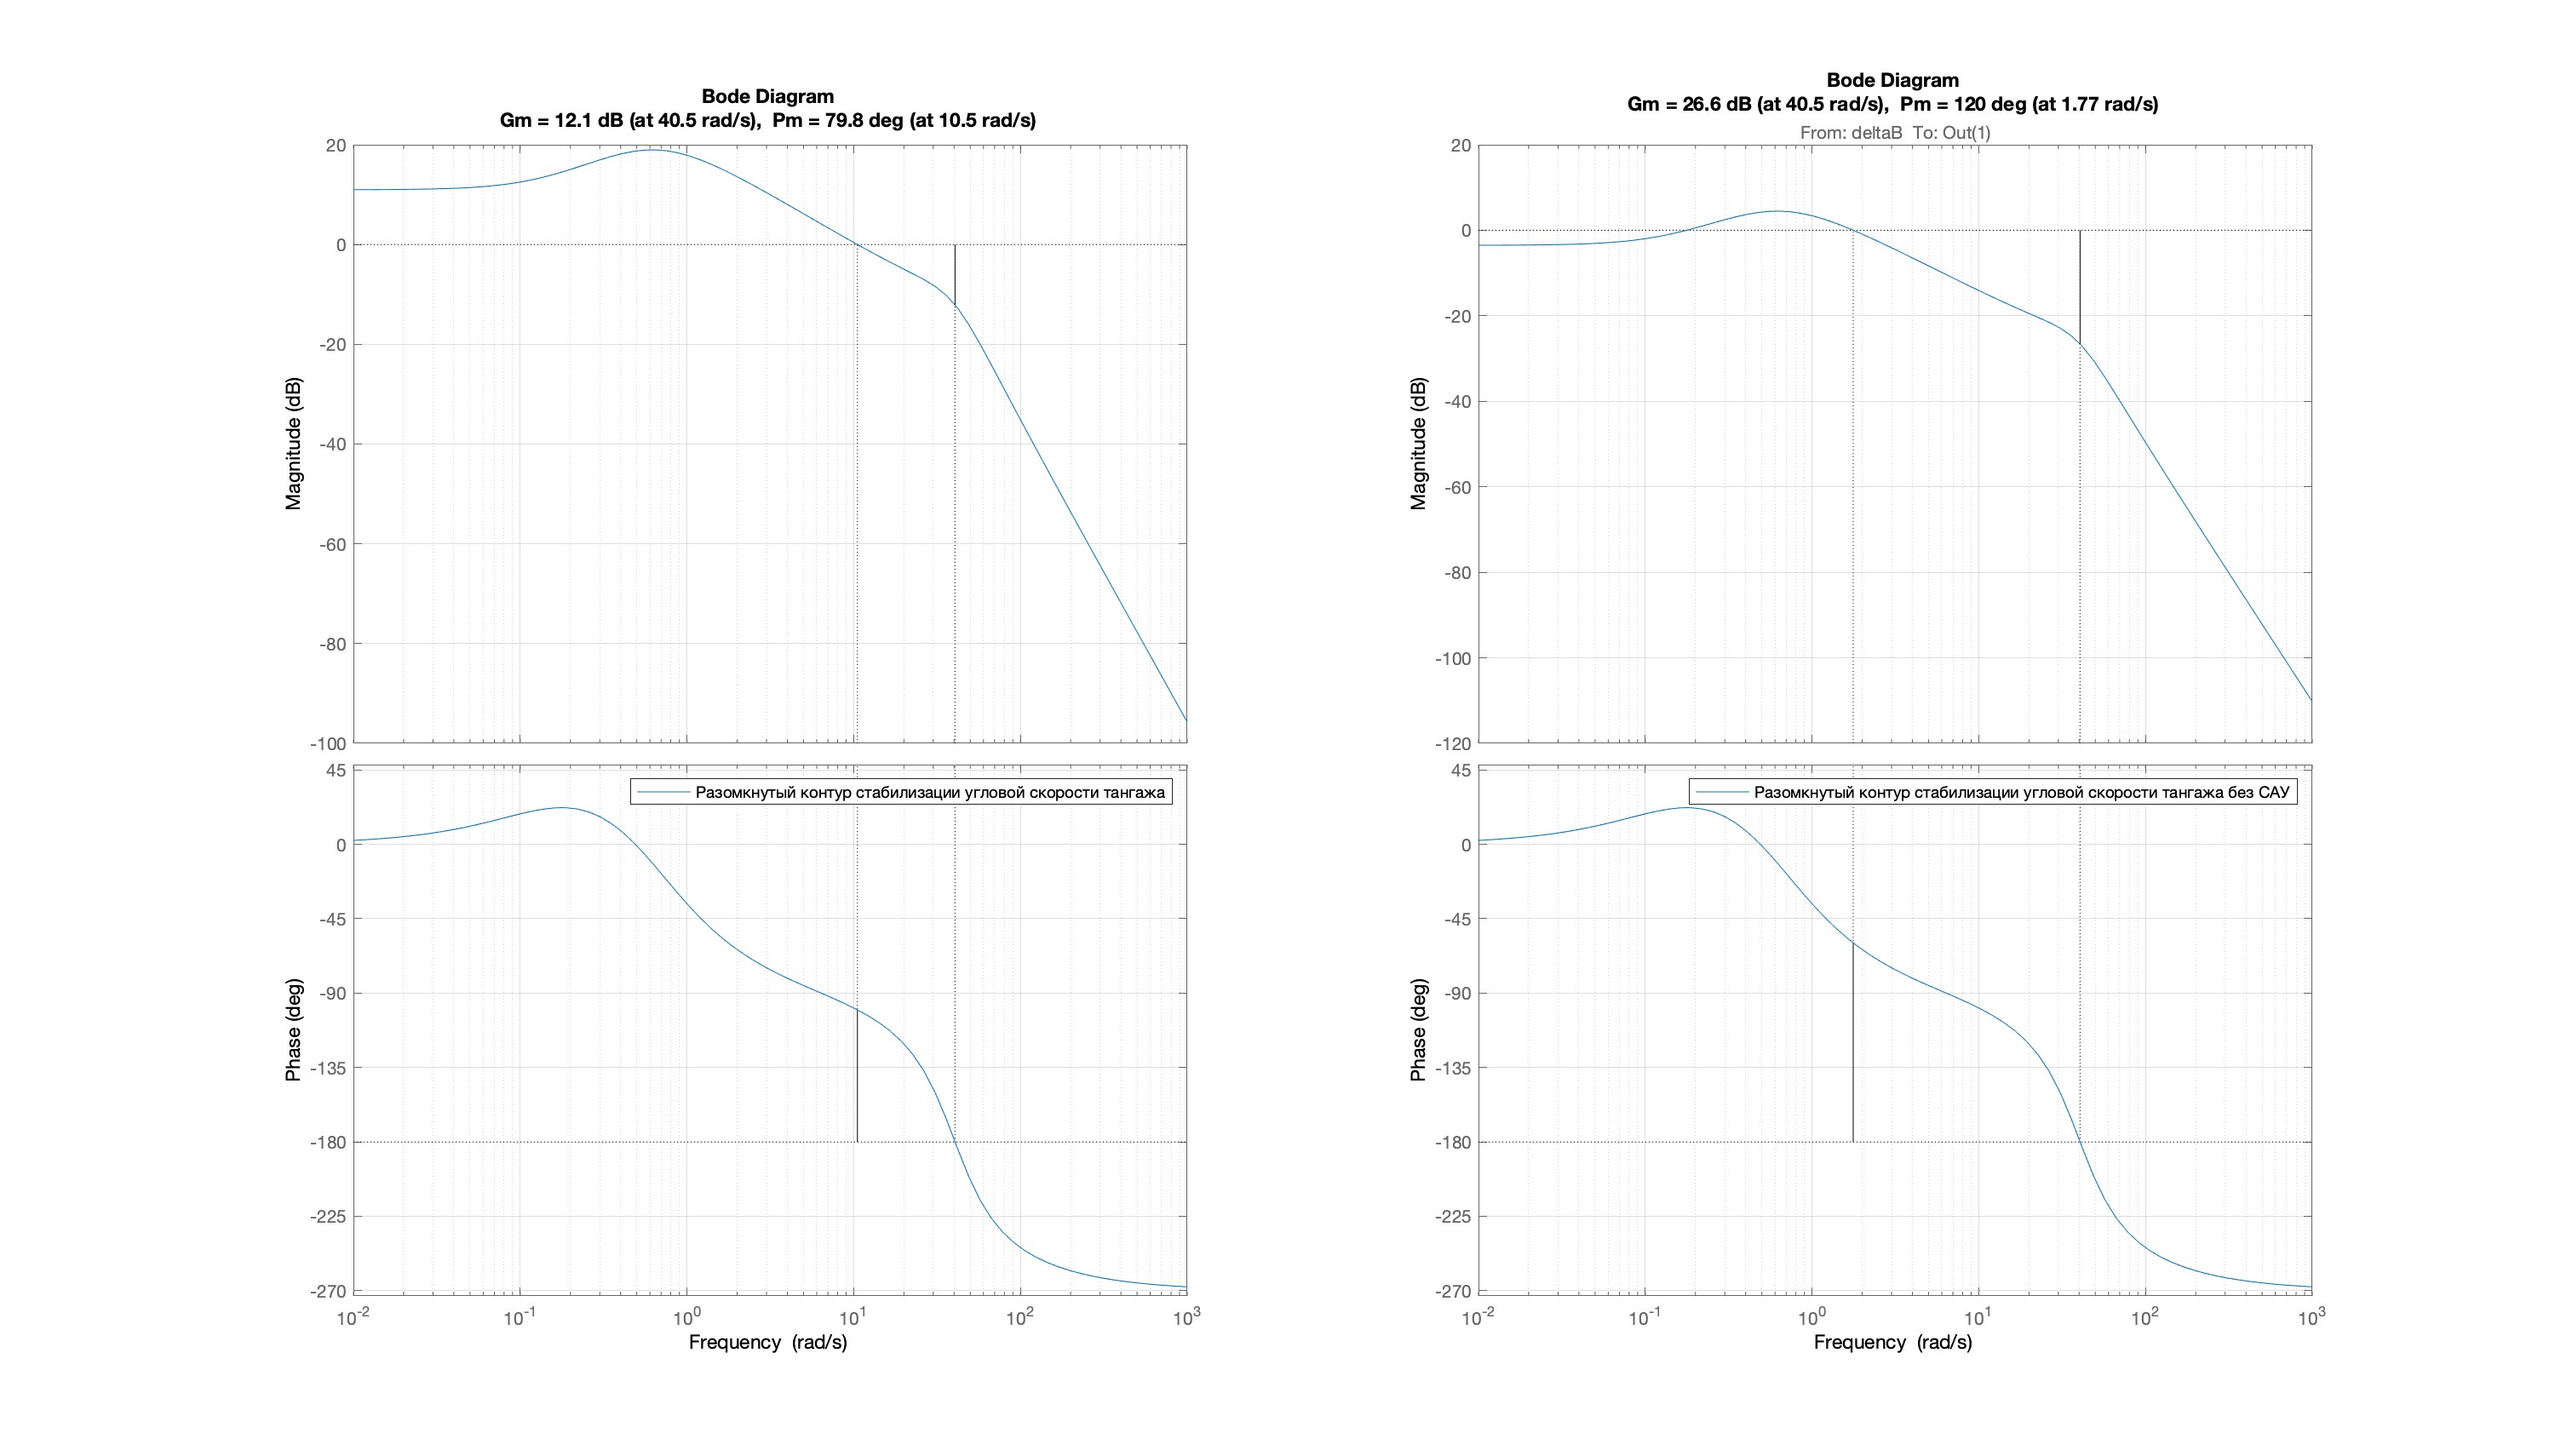
\includegraphics[width=\linewidth]{Оглавление/Part2/Sactions/Content/frequencies/Угловая скорость тангажа раз qMIN.jpg}}
    \caption{ЛАФЧХ разомкнутого контура демпфирования угловой скорости тангажа}
    \label{fig:Угловая скорость тангажа раз qMIN}
\end{figure}

Из рисунка \ref{fig:Угловая скорость тангажа раз qMIN} видно, что до синтеза данного контура запасы устойчивости по амплитуде и по фазе не удовлетворяют заданным требованиям, то есть запас по амплитуде меньше 10 дб и запас по фазе меньше 45 град, а после синтеза $\Delta A = 12,3$дБ $\Delta \varphi = 80^0$, следовательно, синтез проведен успешно, коэффициенты рассчитаны верно. Замкнутая система будет устойчива. Частота среза после синтеза не превысила граничного значения, она находится на участке с наклоном -20дб/дек, чего и требовалось достичь в результате синтеза.  

\begin{center}
    Контур стабилизации тангажа:
\end{center}

\begin{figure}[H]
    \center{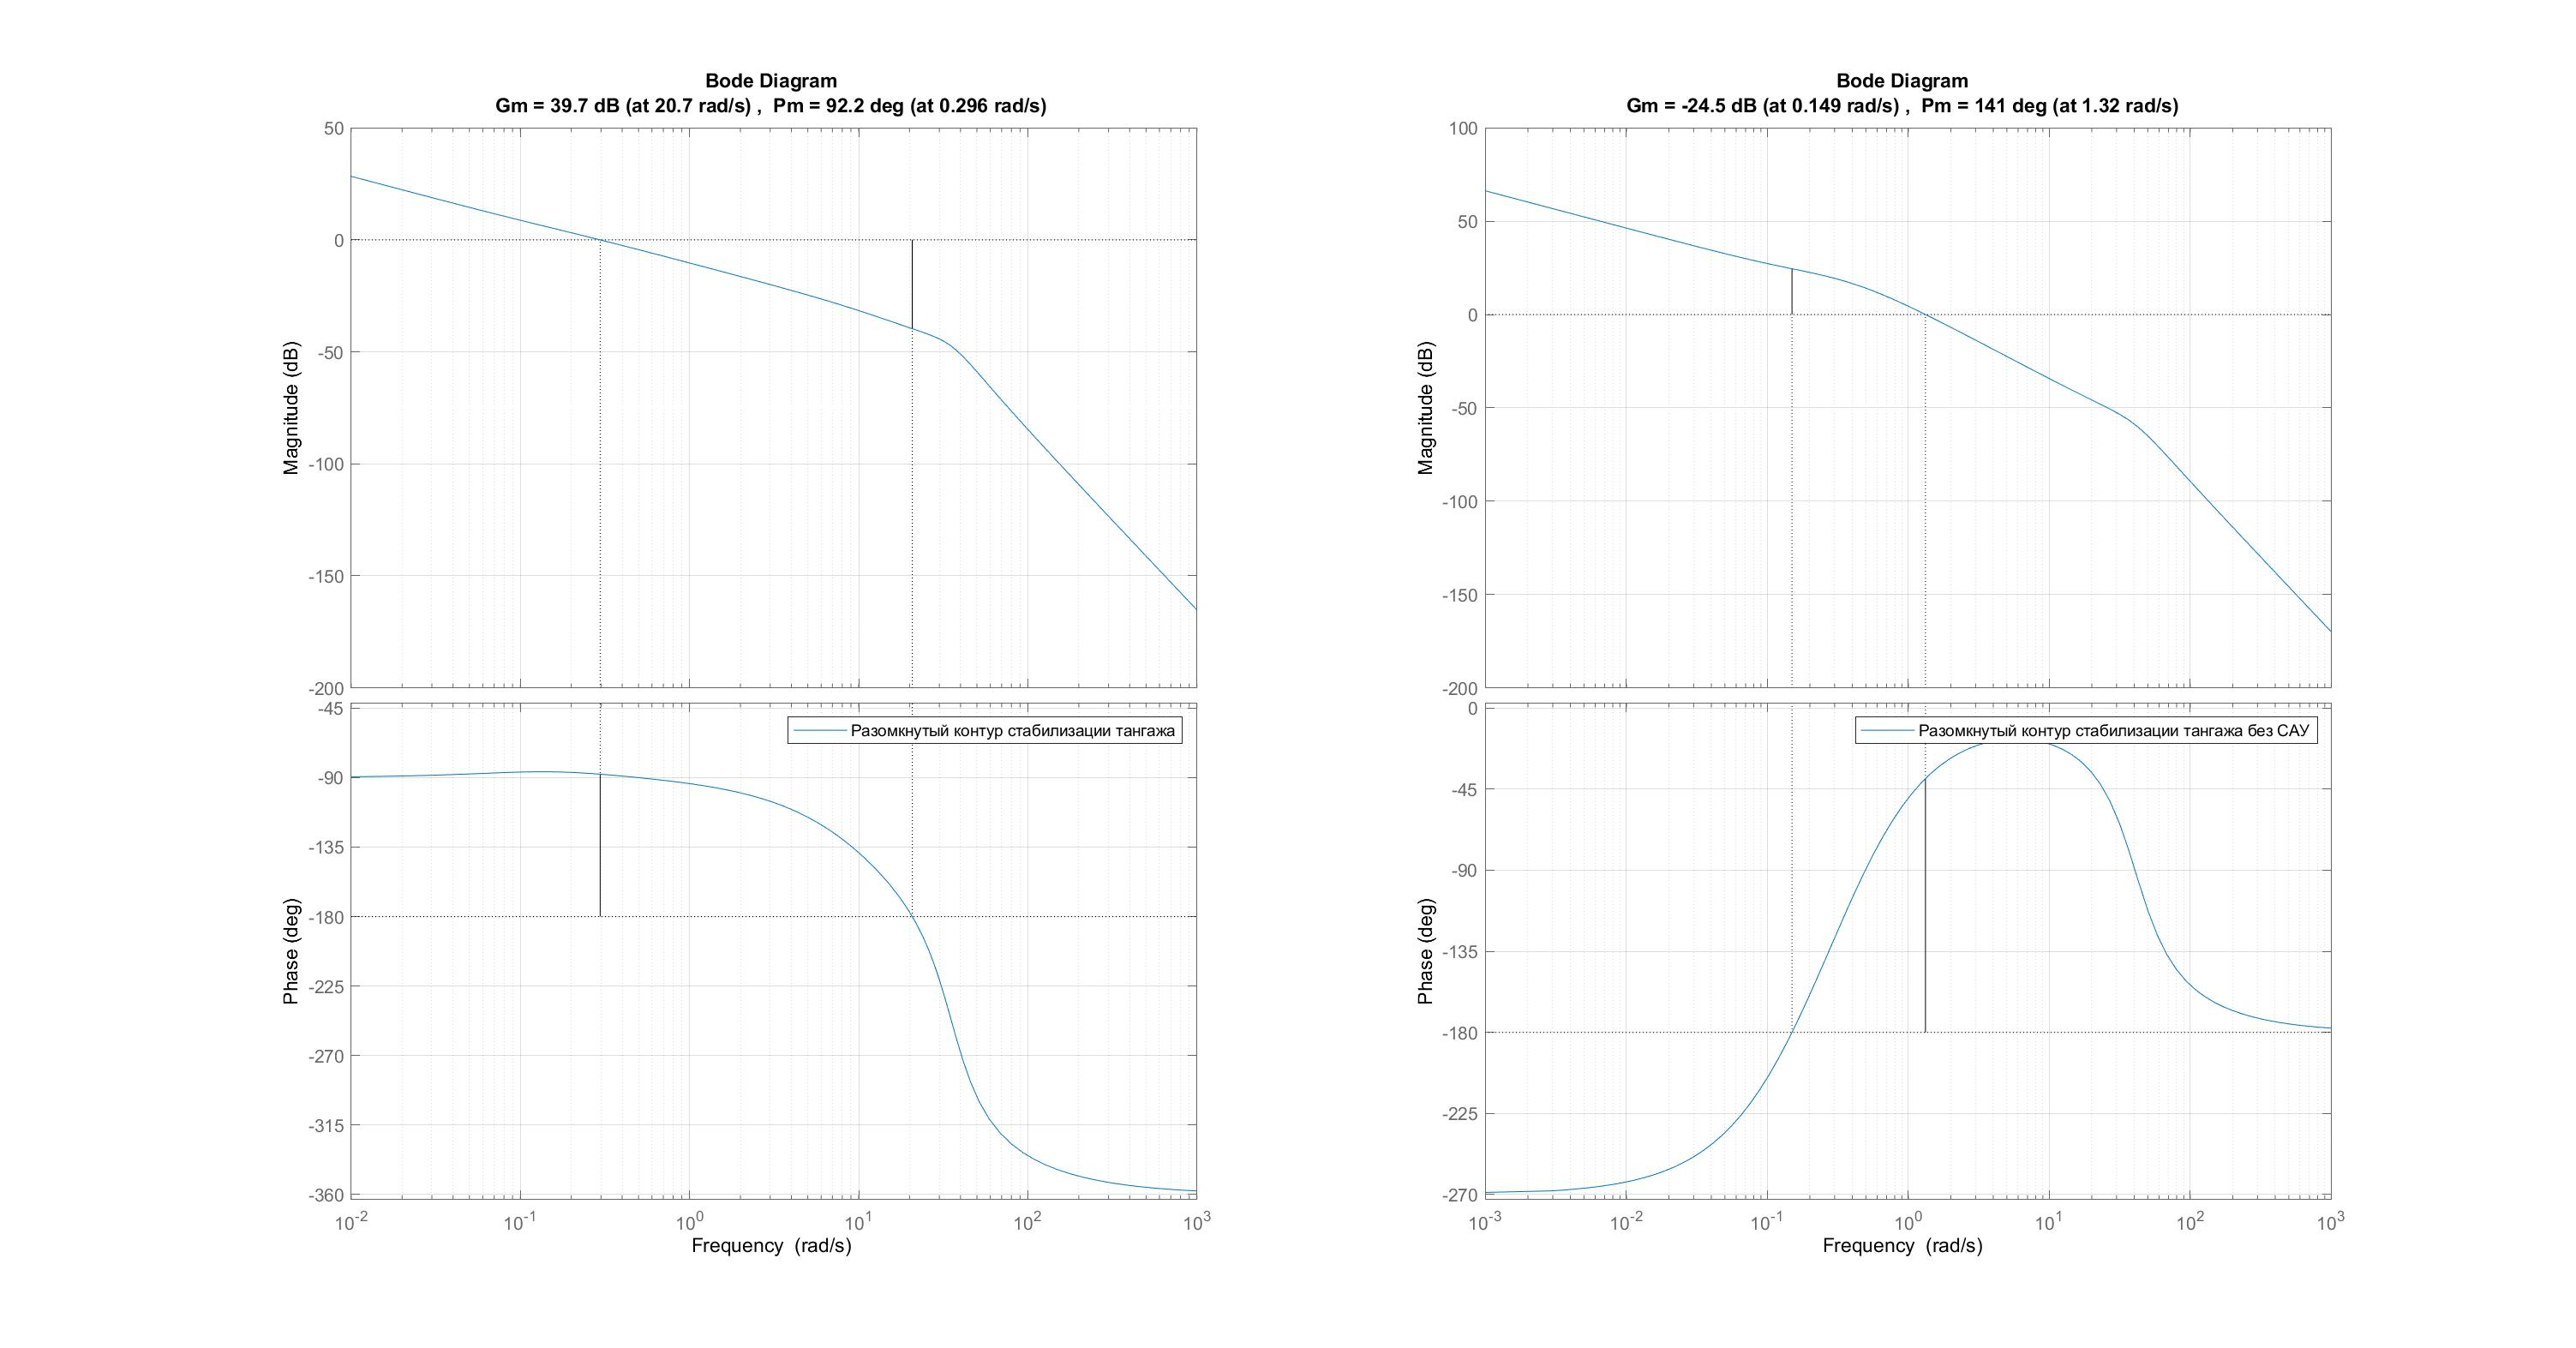
\includegraphics[width=\linewidth]{Оглавление/Part2/Sactions/Content/frequencies/Тангаж раз qMIN.jpg}}
    \caption{ЛАФЧХ разомкнутого контура стабилизации тангажа}
    \label{fig:Тангаж раз qMIN}
\end{figure}

Из рисунка \ref{fig:Тангаж раз qMIN} видно, что до синтеза данного контура запасы устойчивости по амплитуде и по фазе не удовлетворяют заданным требованиям, то есть запас по амплитуде меньше 10 дб и запас по фазе меньше 45 град, а после синтеза $\Delta A = 39,7 $дБ $\Delta \varphi = 92^0$, следовательно, синтез проведен успешно, коэффициенты рассчитаны верно. Замкнутая система будет устойчива.  

\begin{center}
    Контур вертикальной скорости:
\end{center}

\begin{figure}[H]
    \center{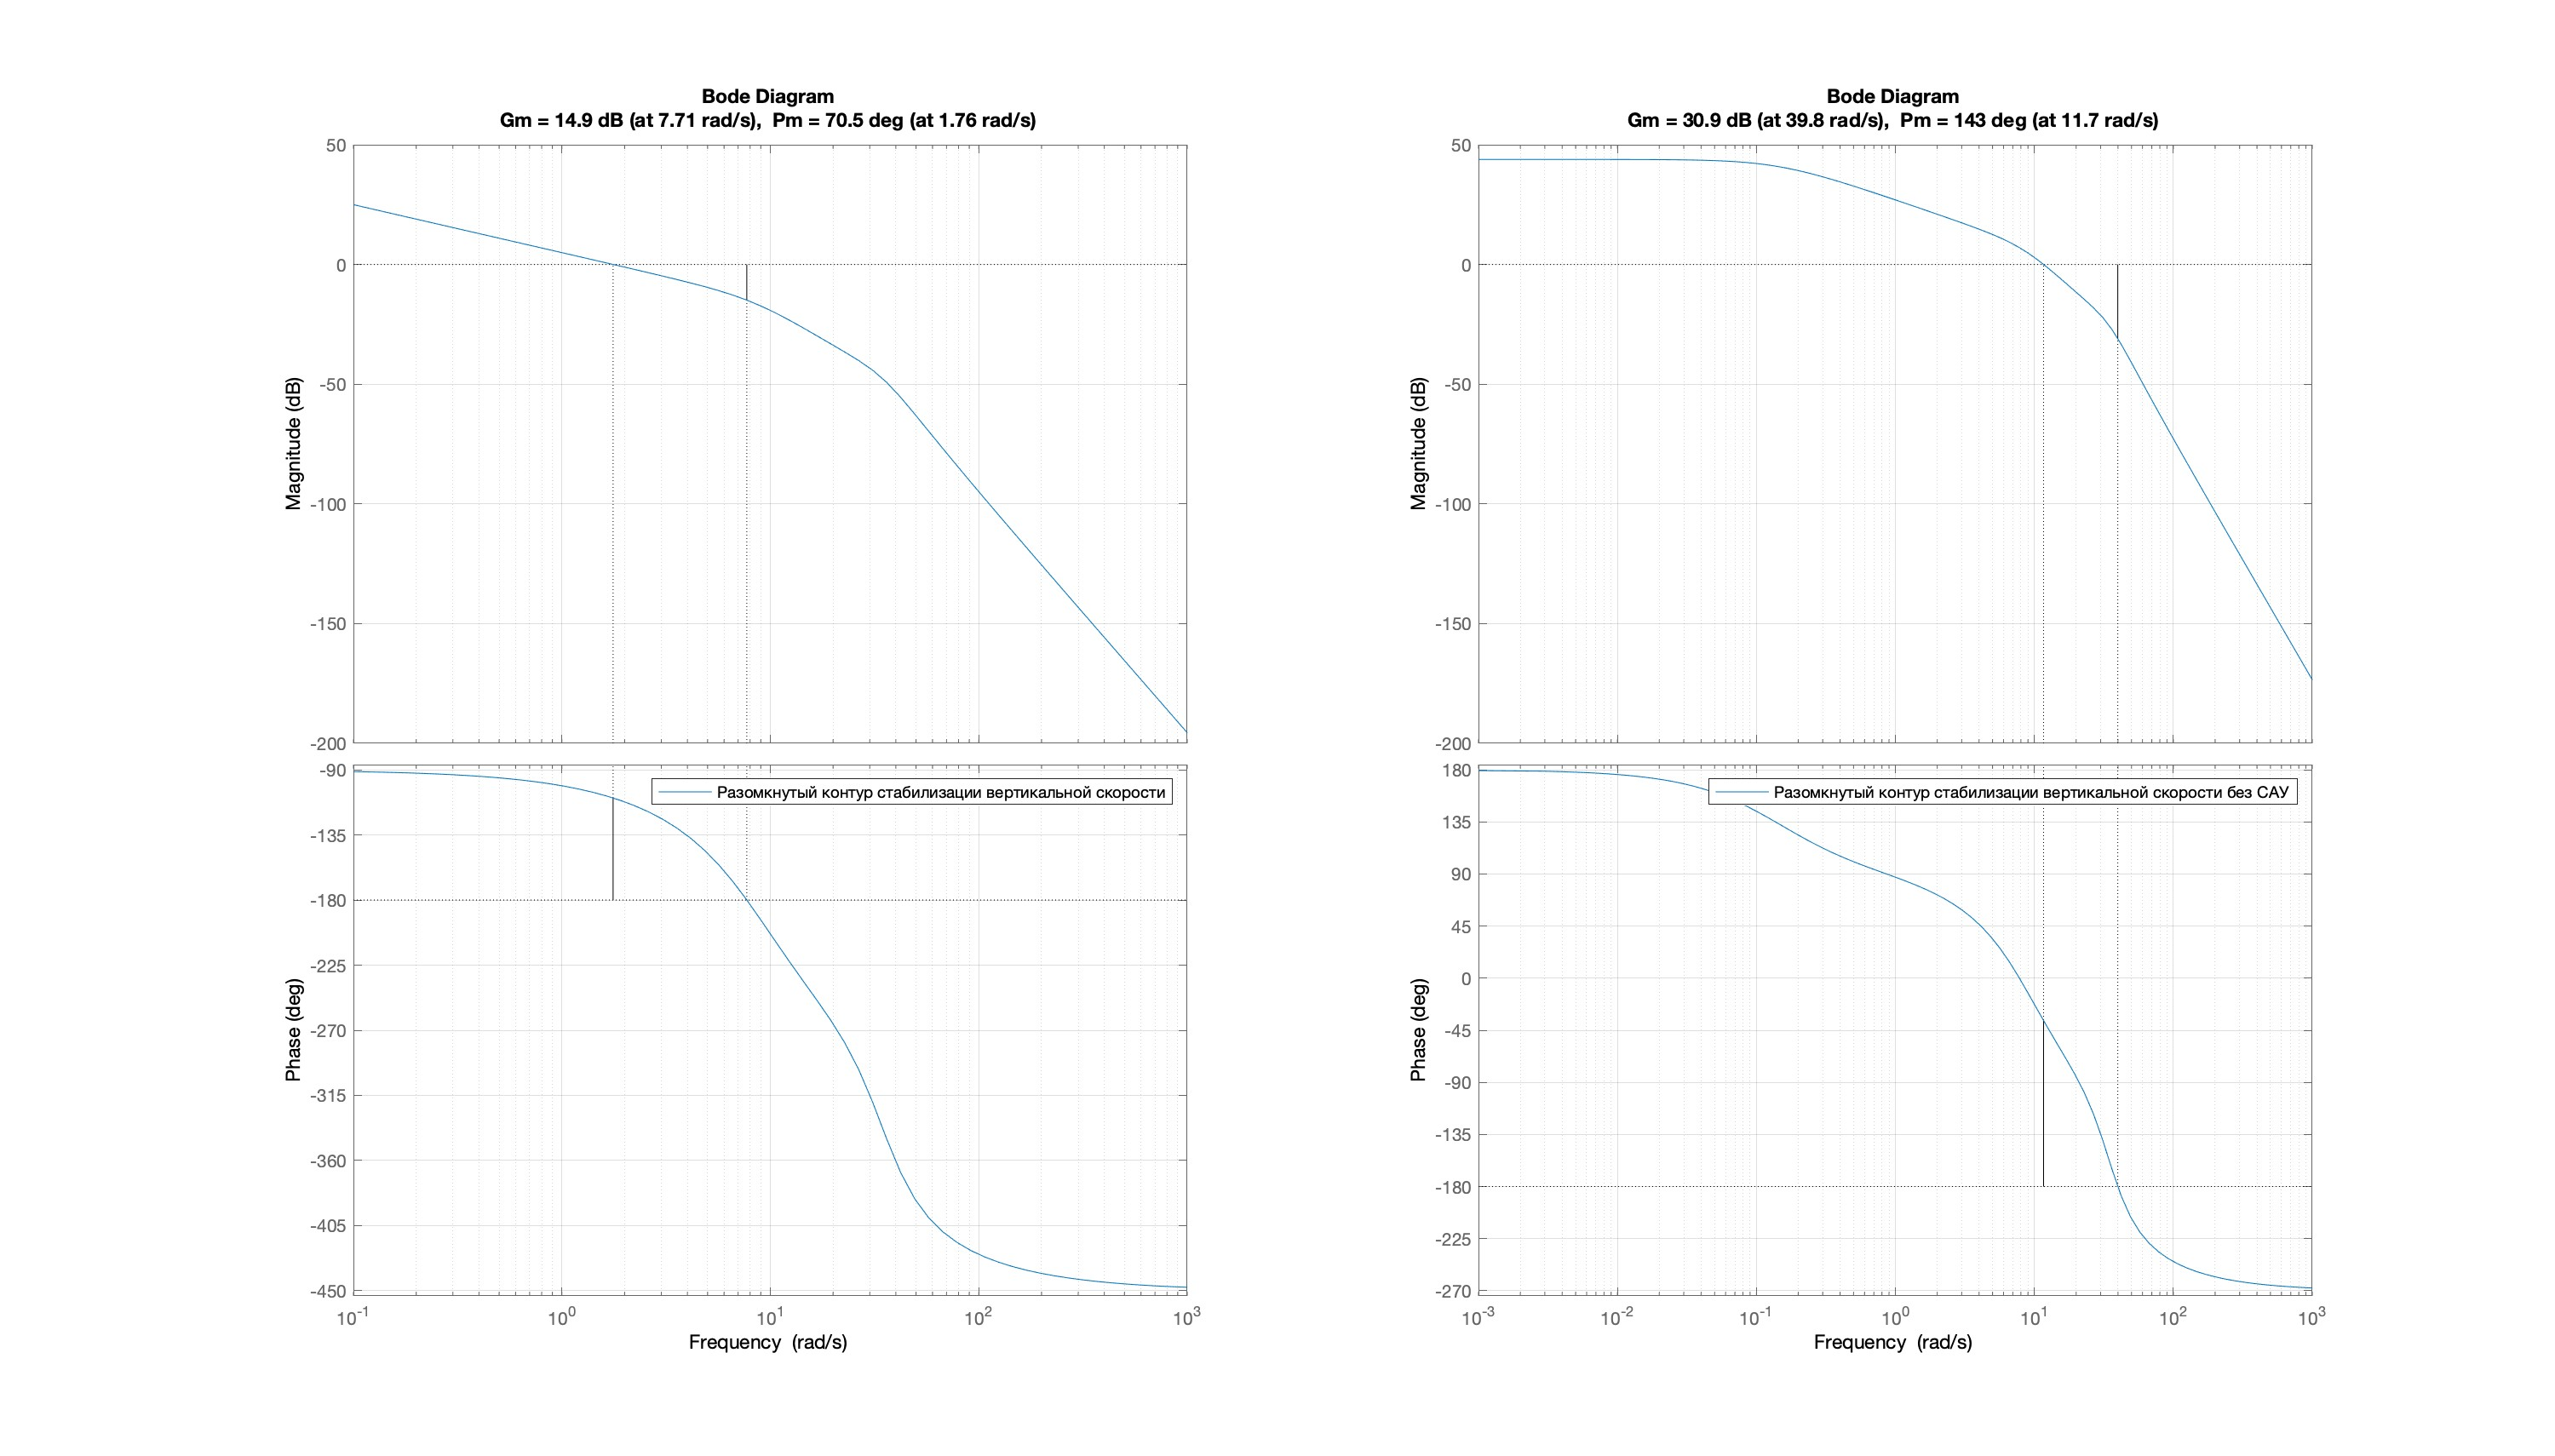
\includegraphics[width=\linewidth]{Оглавление/Part2/Sactions/Content/frequencies/Вертикальная скорость раз qMIN.jpg}}
    \caption{ЛАФЧХ разомкнутого контура стабилизации вертикальной скорости}
    \label{fig:Вертикальная скорость раз qMIN}
\end{figure}

Из рисунка \ref{fig:Вертикальная скорость раз qMIN} видно, что после синтеза $\Delta A = 42,2 $дБ $\Delta \varphi = 73^0$, следовательно, синтез проведен успешно, коэффициенты рассчитаны верно. Замкнутая система будет устойчива. 

\begin{figure}[H]
    \center{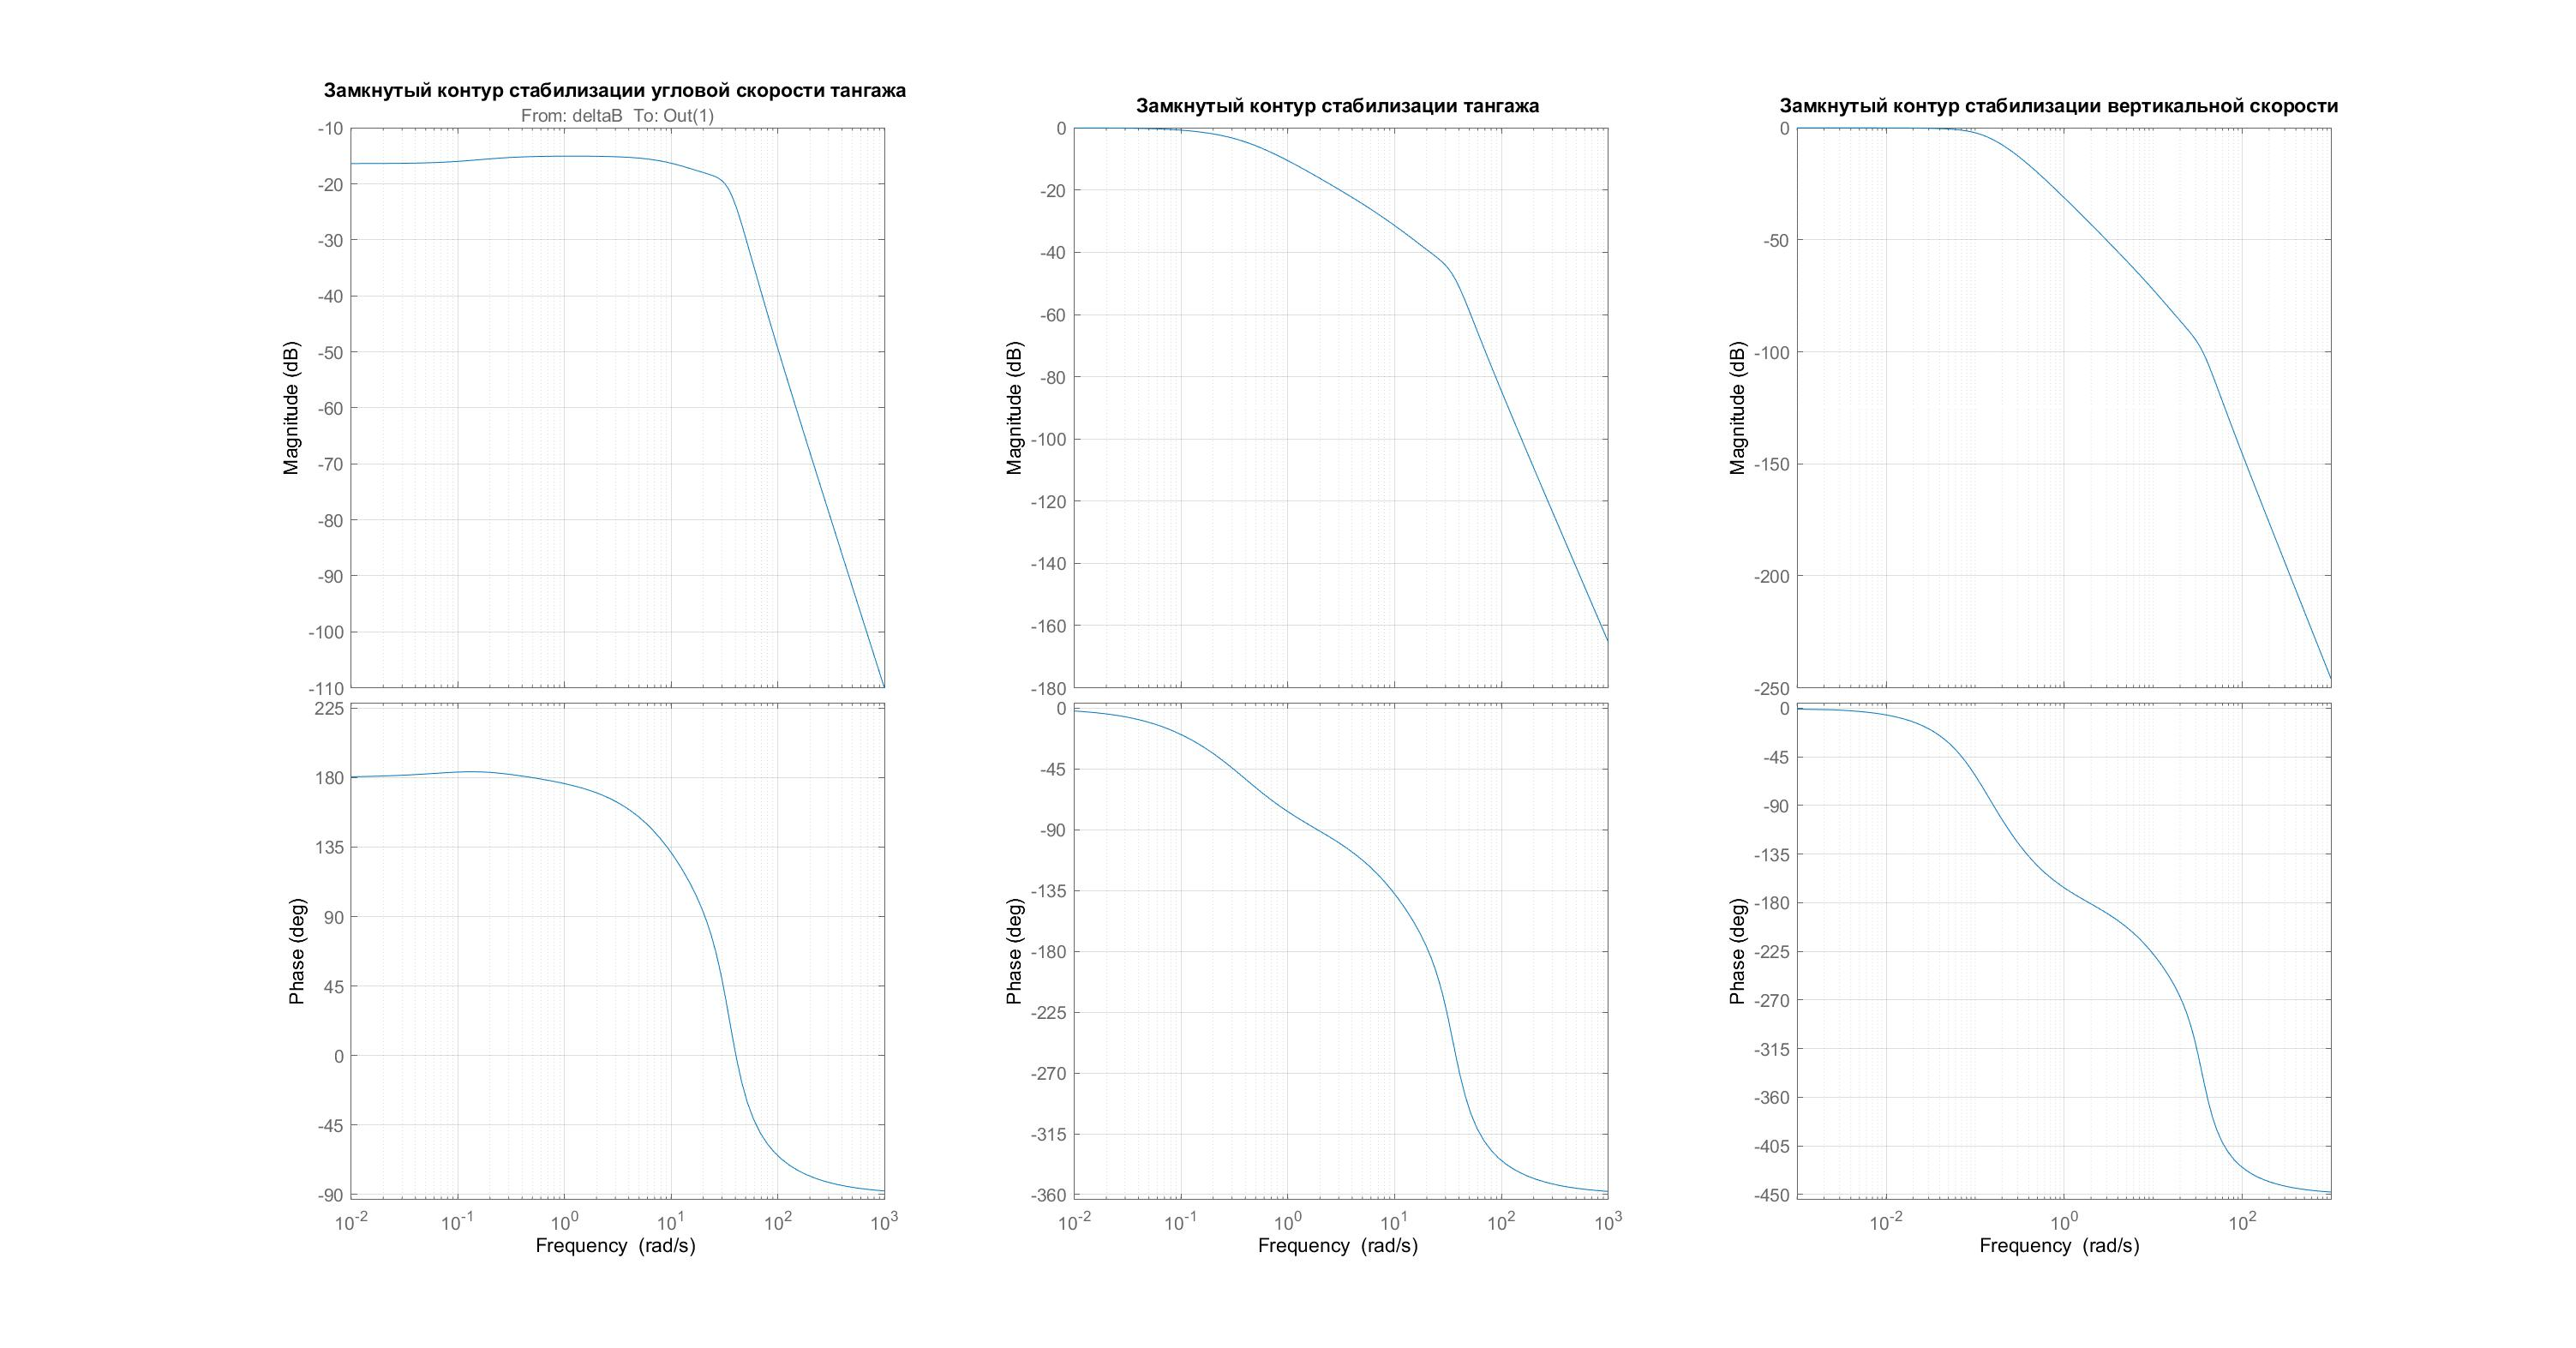
\includegraphics[width=\linewidth]{Оглавление/Part2/Sactions/Content/frequencies/ZAM qMIN.jpg}}
    \caption{ЛАФЧХ замкнутого контура }
    \label{fig:Вертикальная скорость зам qMIN}
\end{figure}
% __________________________________________________________________________________________
\subsubsubsection{Частотный анализ $q_{max}$}

\begin{center}
    Контур демпфирования угловой скорости тангажа:
\end{center}

\begin{figure}[H]
    \center{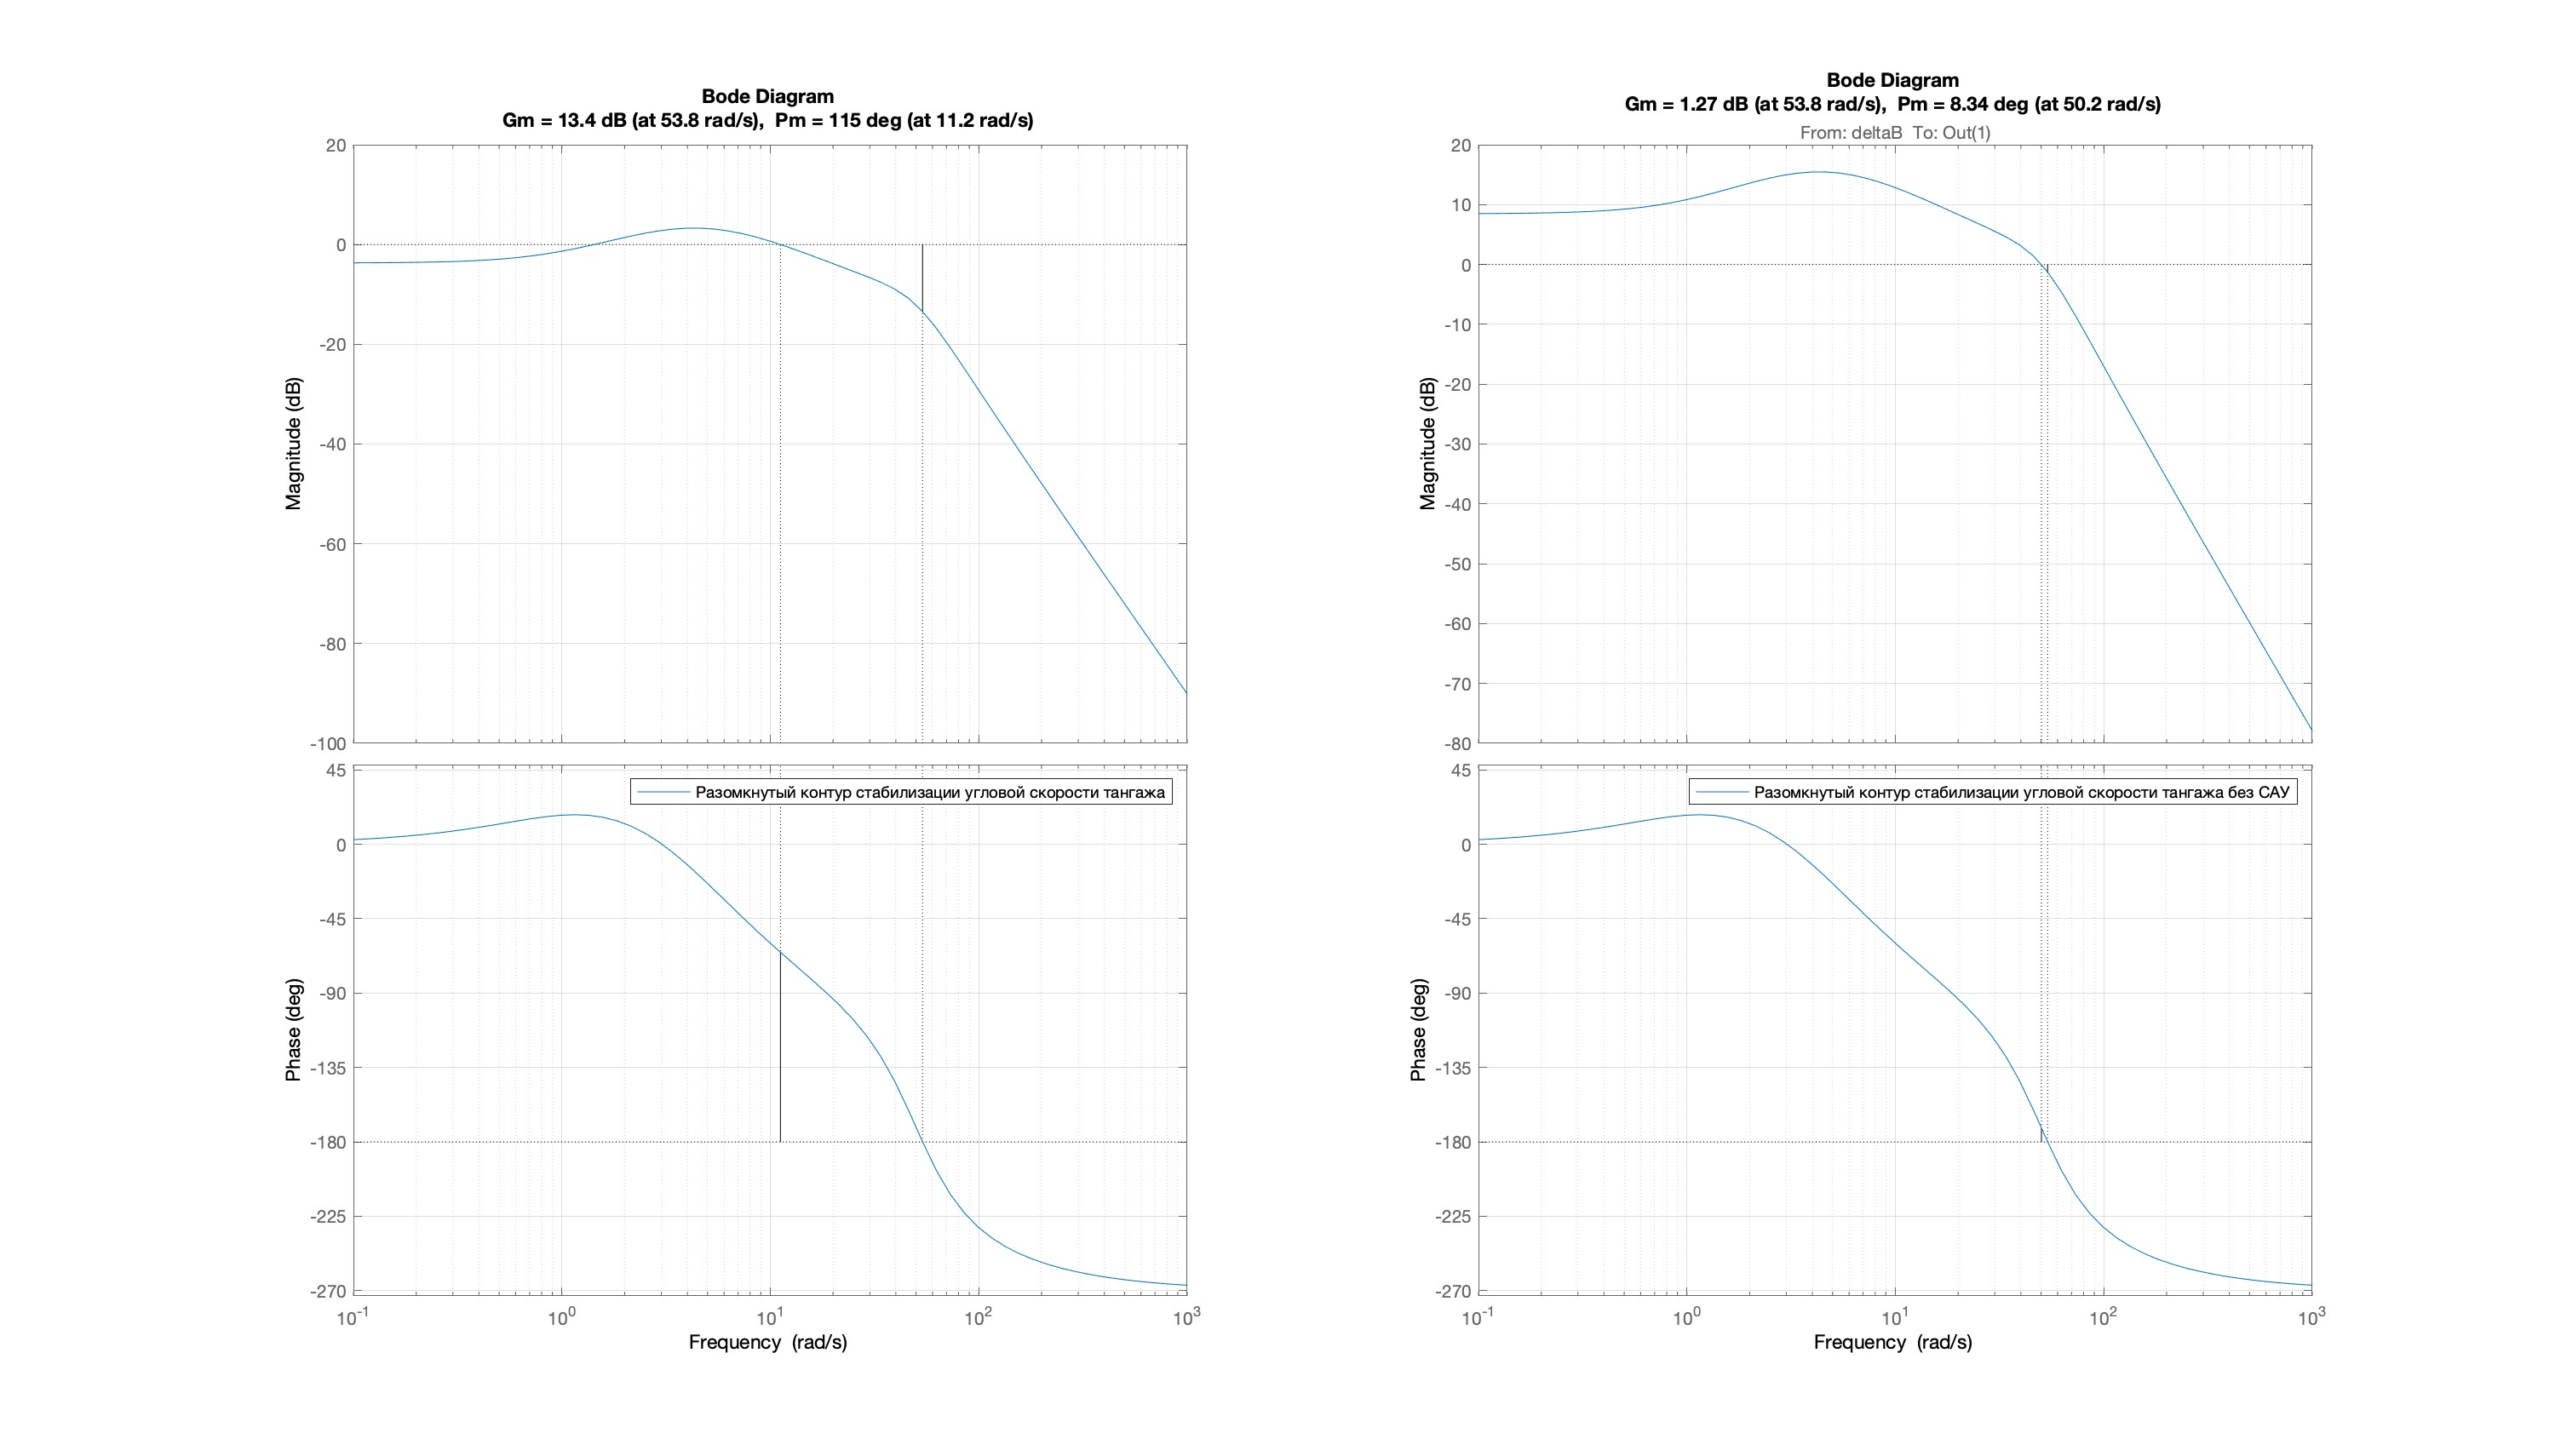
\includegraphics[width=\linewidth]{Оглавление/Part2/Sactions/Content/frequencies/Угловая скорость тангажа раз qMAX.jpg}}
    \caption{ЛАФЧХ разомкнутого контура демпфирования угловой скорости тангажа}
    \label{fig:Угловая скорость тангажа раз qMAX}
\end{figure}

Из рисунка \ref{fig:Угловая скорость тангажа раз qMAX} видно, что до синтеза данного контура запасы устойчивости по амплитуде и по фазе не удовлетворяют заданным требованиям, то есть запас по амплитуде меньше 10 дб и запас по фазе меньше 45 град, а после синтеза $\Delta A = 13,7 $дБ $\Delta \varphi = 124^0$, следовательно, синтез проведен успешно, коэффициенты рассчитаны верно. Замкнутая система будет устойчива. Частота среза после синтеза не превысила граничного значения, она находится на участке с наклоном -20дб/дек, чего и требовалось достичь в результате синтеза.  

\begin{center}
    Контур стабилизации тангажа:
\end{center}

\begin{figure}[H]
    \center{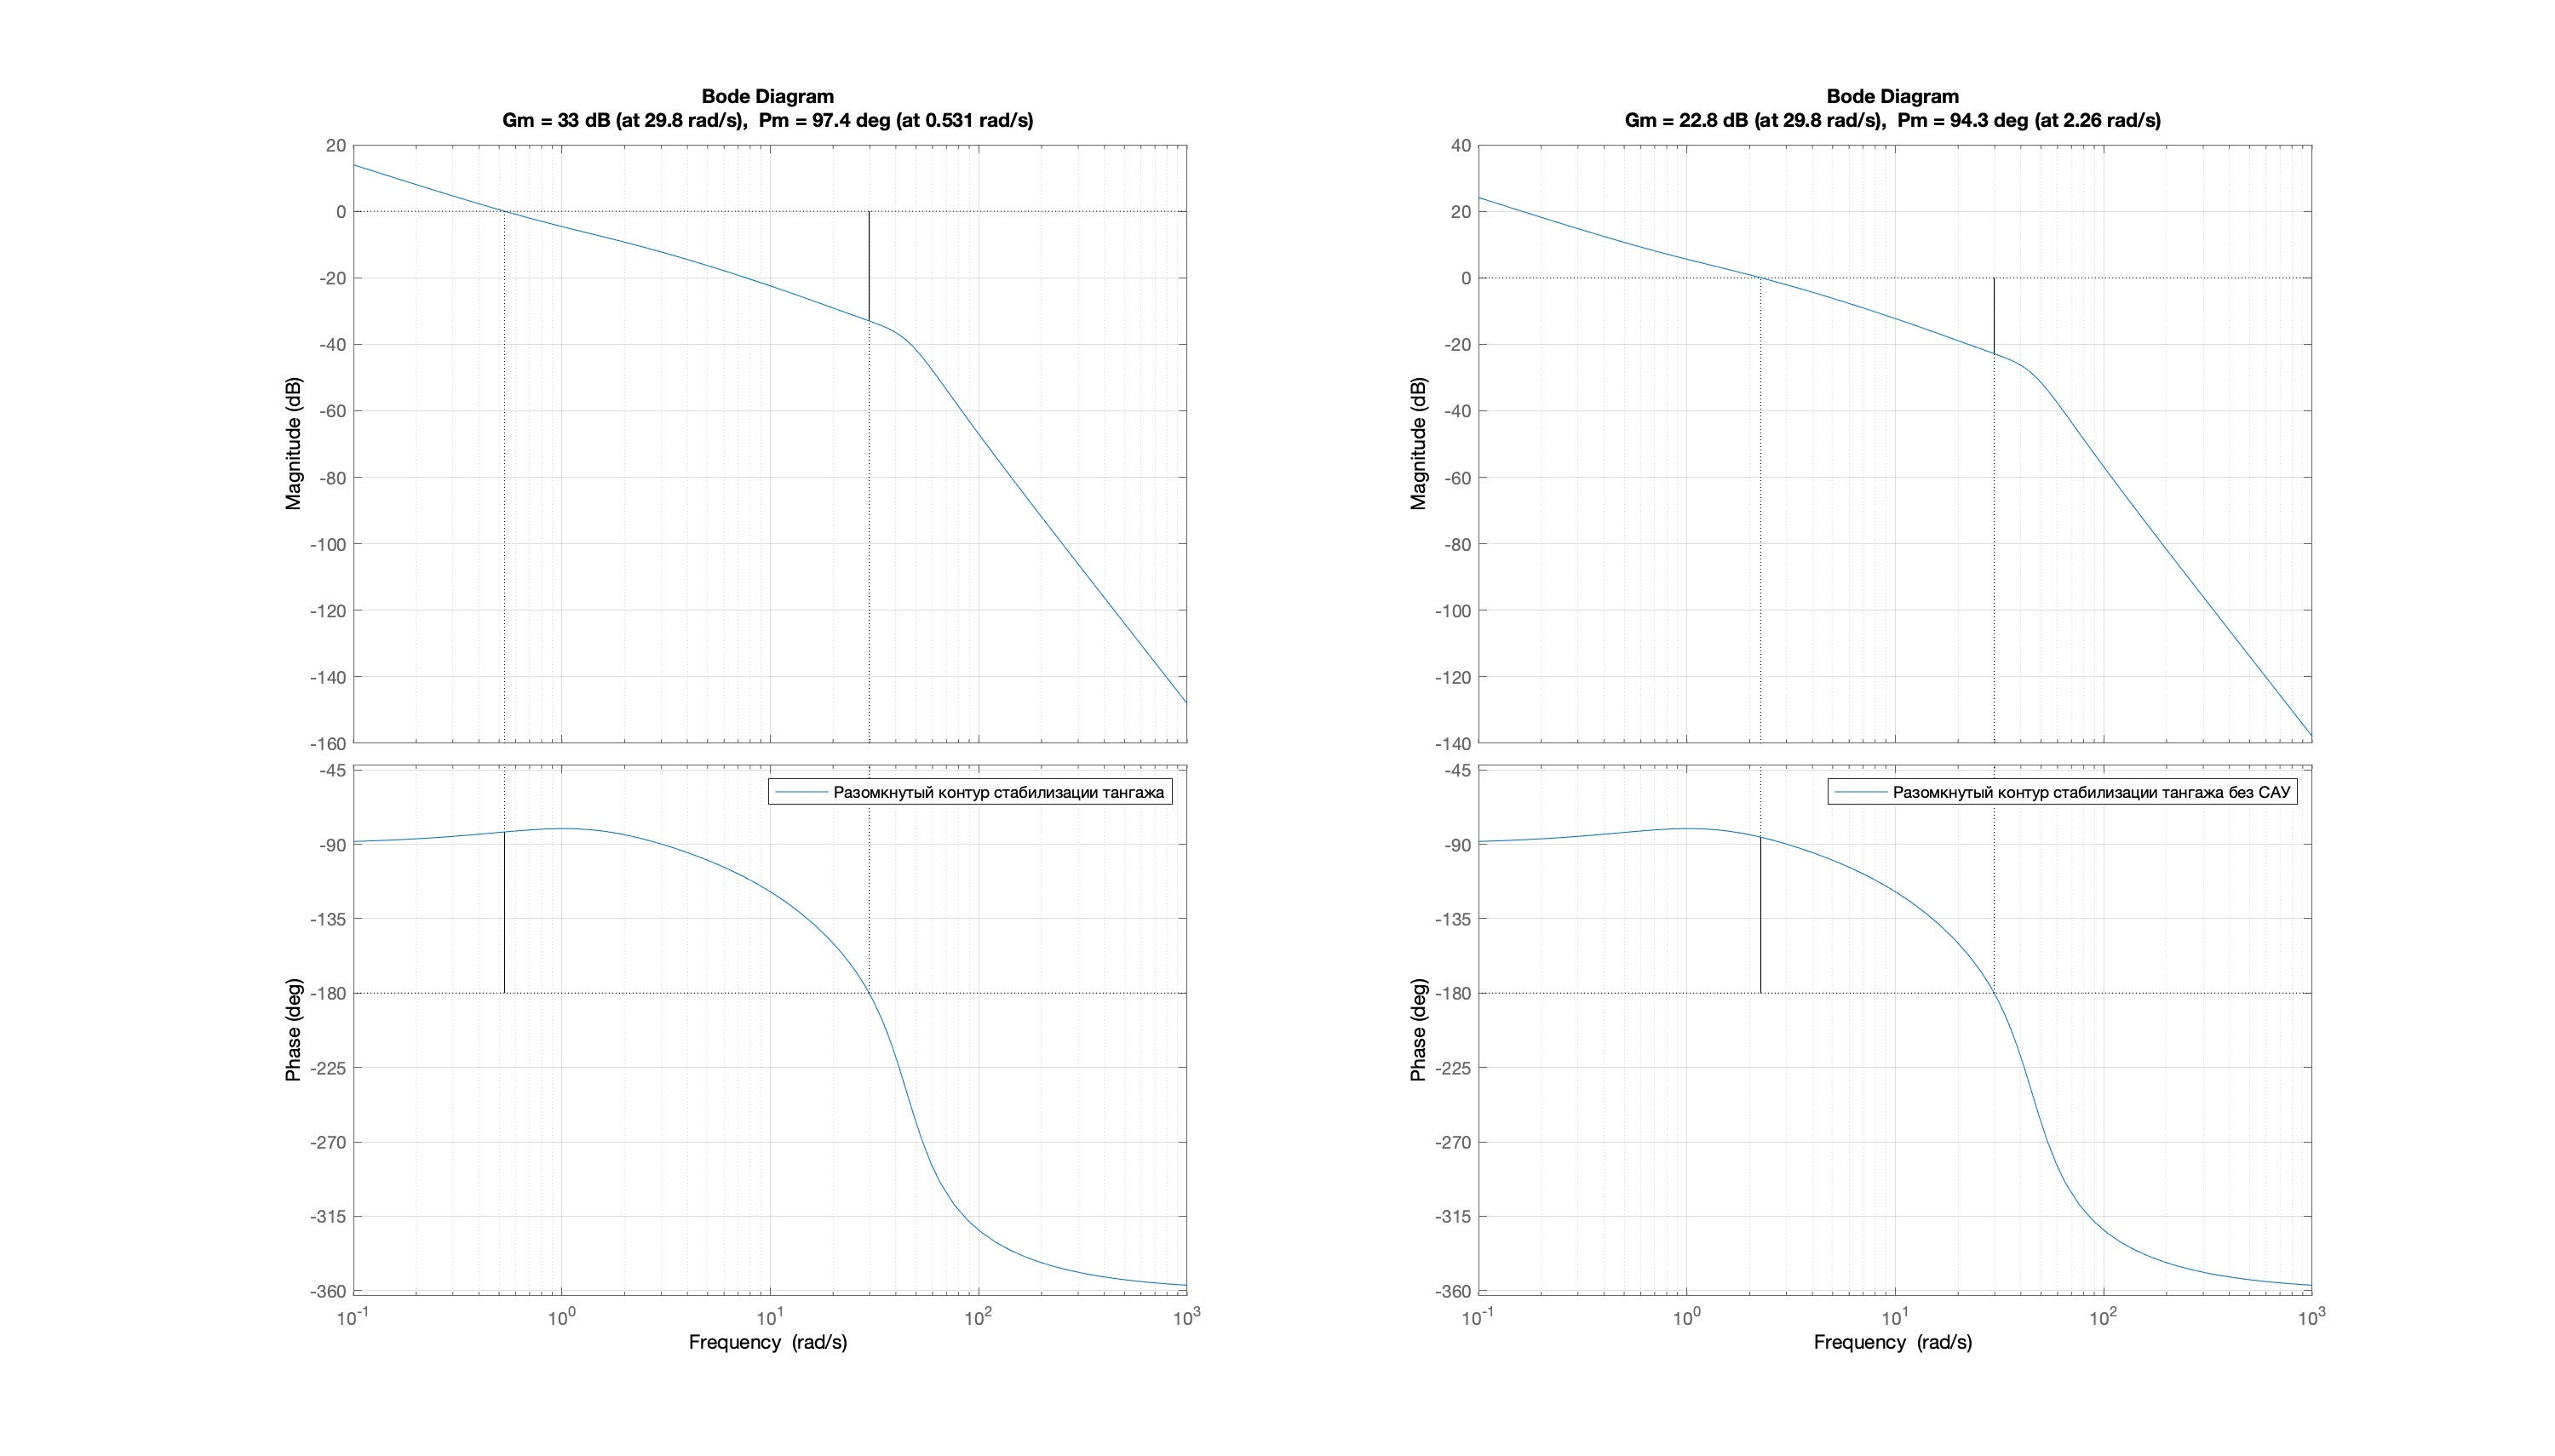
\includegraphics[width=\linewidth]{Оглавление/Part2/Sactions/Content/frequencies/Тангаж раз qMAX.jpg}}
    \caption{ЛАФЧХ разомкнутого контура стабилизации тангажа}
    \label{fig:Тангаж раз qMAX}
\end{figure}

Из рисунка \ref{fig:Тангаж раз qMAX} видно, что до синтеза данного контура запасы устойчивости по амплитуде и по фазе не удовлетворяют заданным требованиям, то есть запас по амплитуде меньше 10 дб и запас по фазе меньше 45 град, а после синтеза $\Delta A = 32,3 $дБ $\Delta \varphi = 95,9^0$, следовательно, синтез проведен успешно, коэффициенты рассчитаны верно. Замкнутая система будет устойчива.  

\begin{center}
    Контур вертикальной скорости:
\end{center}

\begin{figure}[H]
    \center{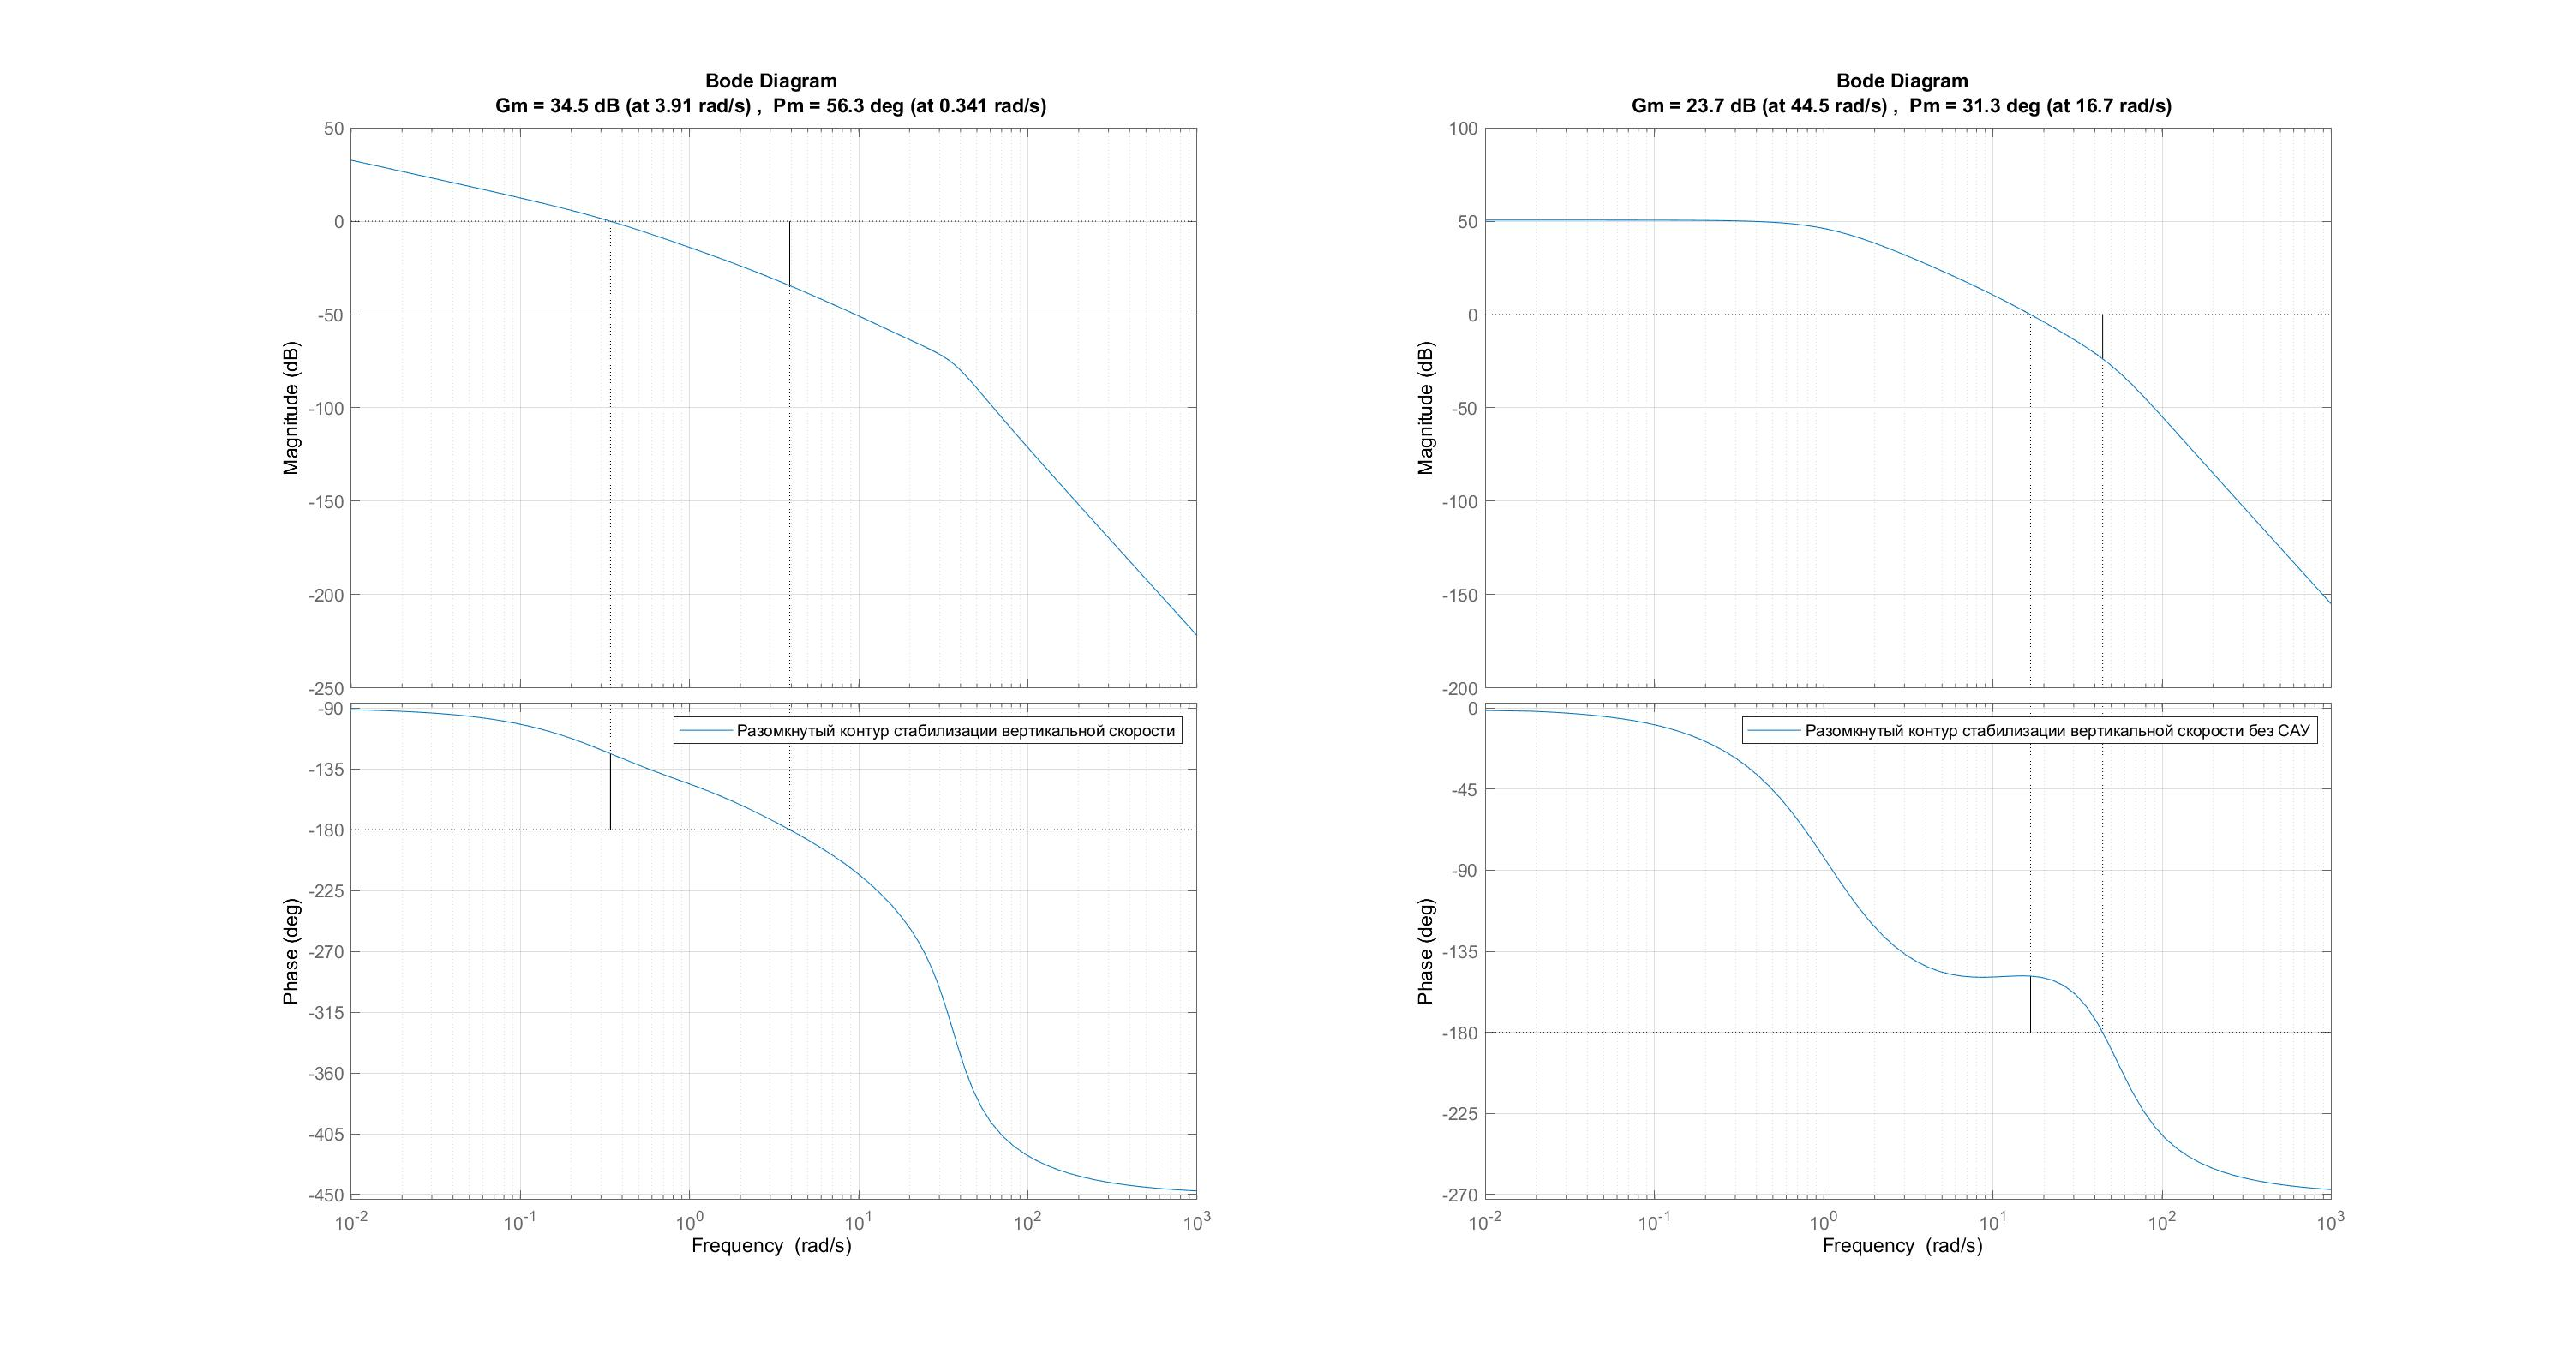
\includegraphics[width=\linewidth]{Оглавление/Part2/Sactions/Content/frequencies/Вертикальная скорость раз qMAX.jpg}}
    \caption{ЛАФЧХ разомкнутого контура стабилизации вертикальной скорости}
    \label{fig:Вертикальная скорость раз qMAX}
\end{figure}

Из рисунка \ref{fig:Вертикальная скорость раз qMAX} видно, что после синтеза $\Delta A = 34,5 $дБ $\Delta \varphi = 56,3^0$, следовательно, синтез проведен успешно, коэффициенты рассчитаны верно. Замкнутая система будет устойчива.  

\begin{figure}[H]
    \center{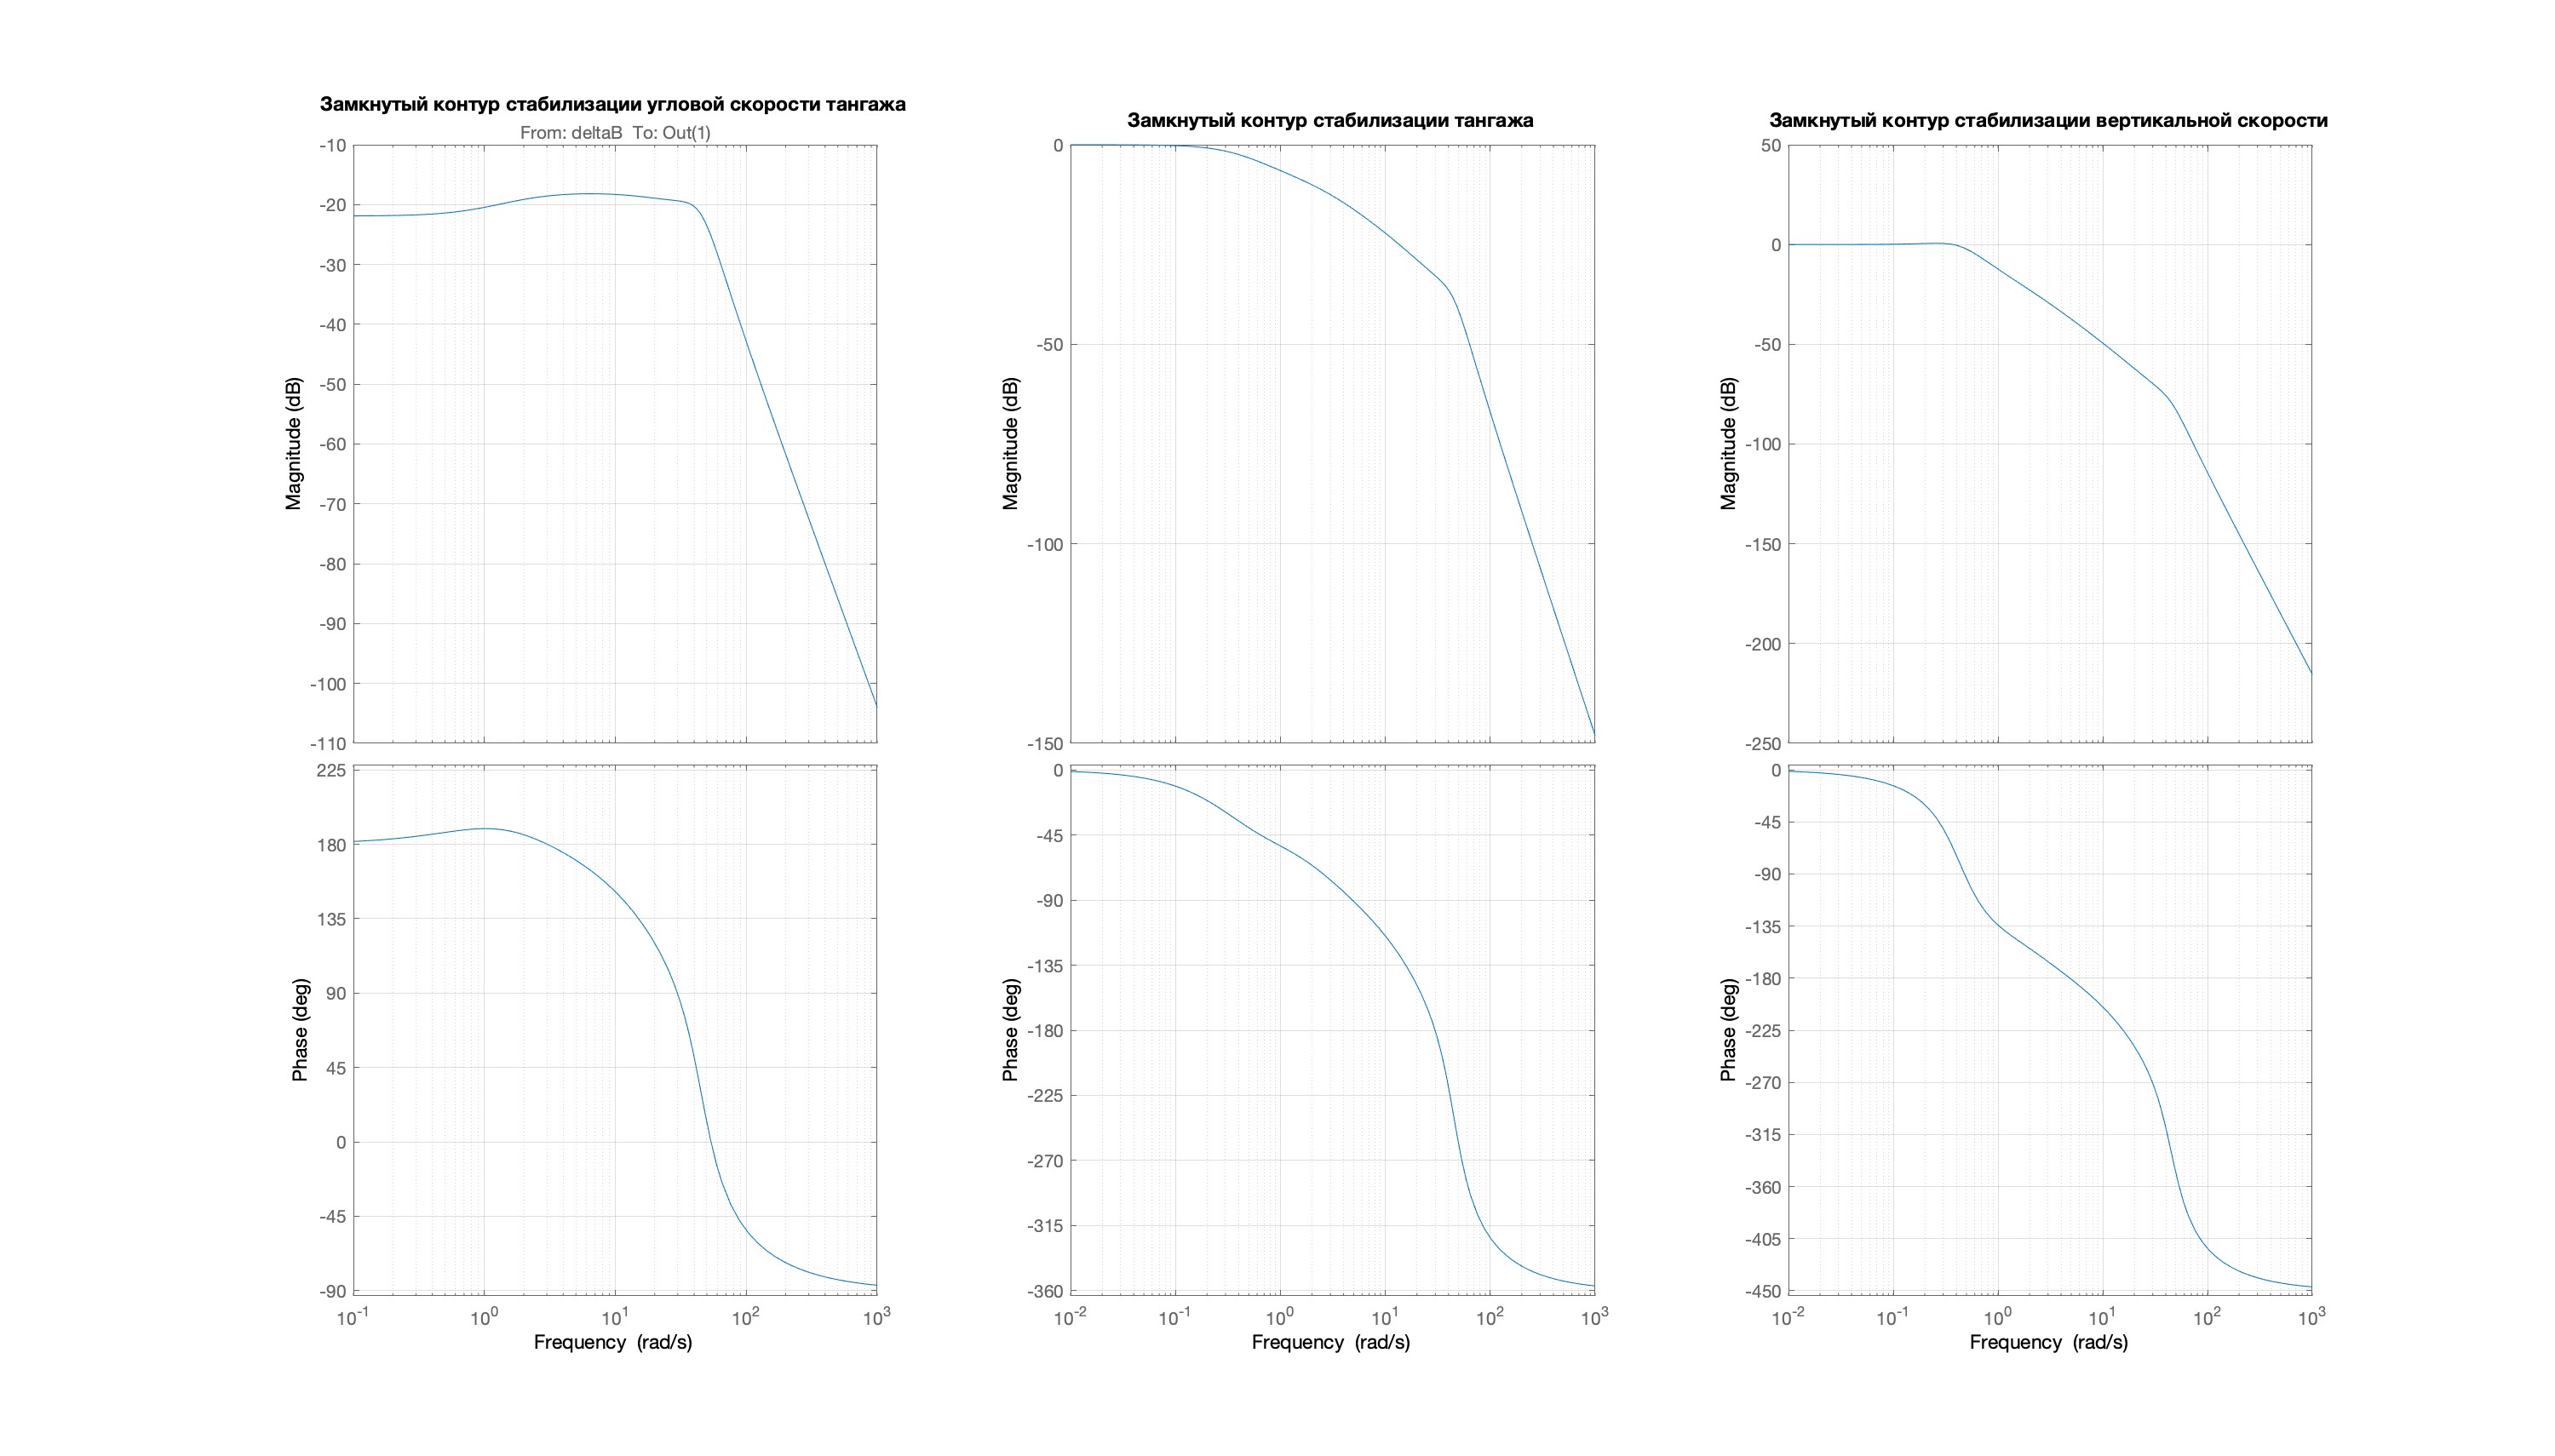
\includegraphics[width=\linewidth]{Оглавление/Part2/Sactions/Content/frequencies/ZAM qMAX.jpg}}
    \caption{ЛАФЧХ замкнутого контура }
    \label{fig:Вертикальная скорость зам qMAX}
\end{figure}

% __________________________________________________________________________________________
\subsubsubsection{Частотный анализ $q_{\text{кр}}$}

\begin{center}
    Контур демпфирования угловой скорости тангажа:
\end{center}

\begin{figure}[H]
    \center{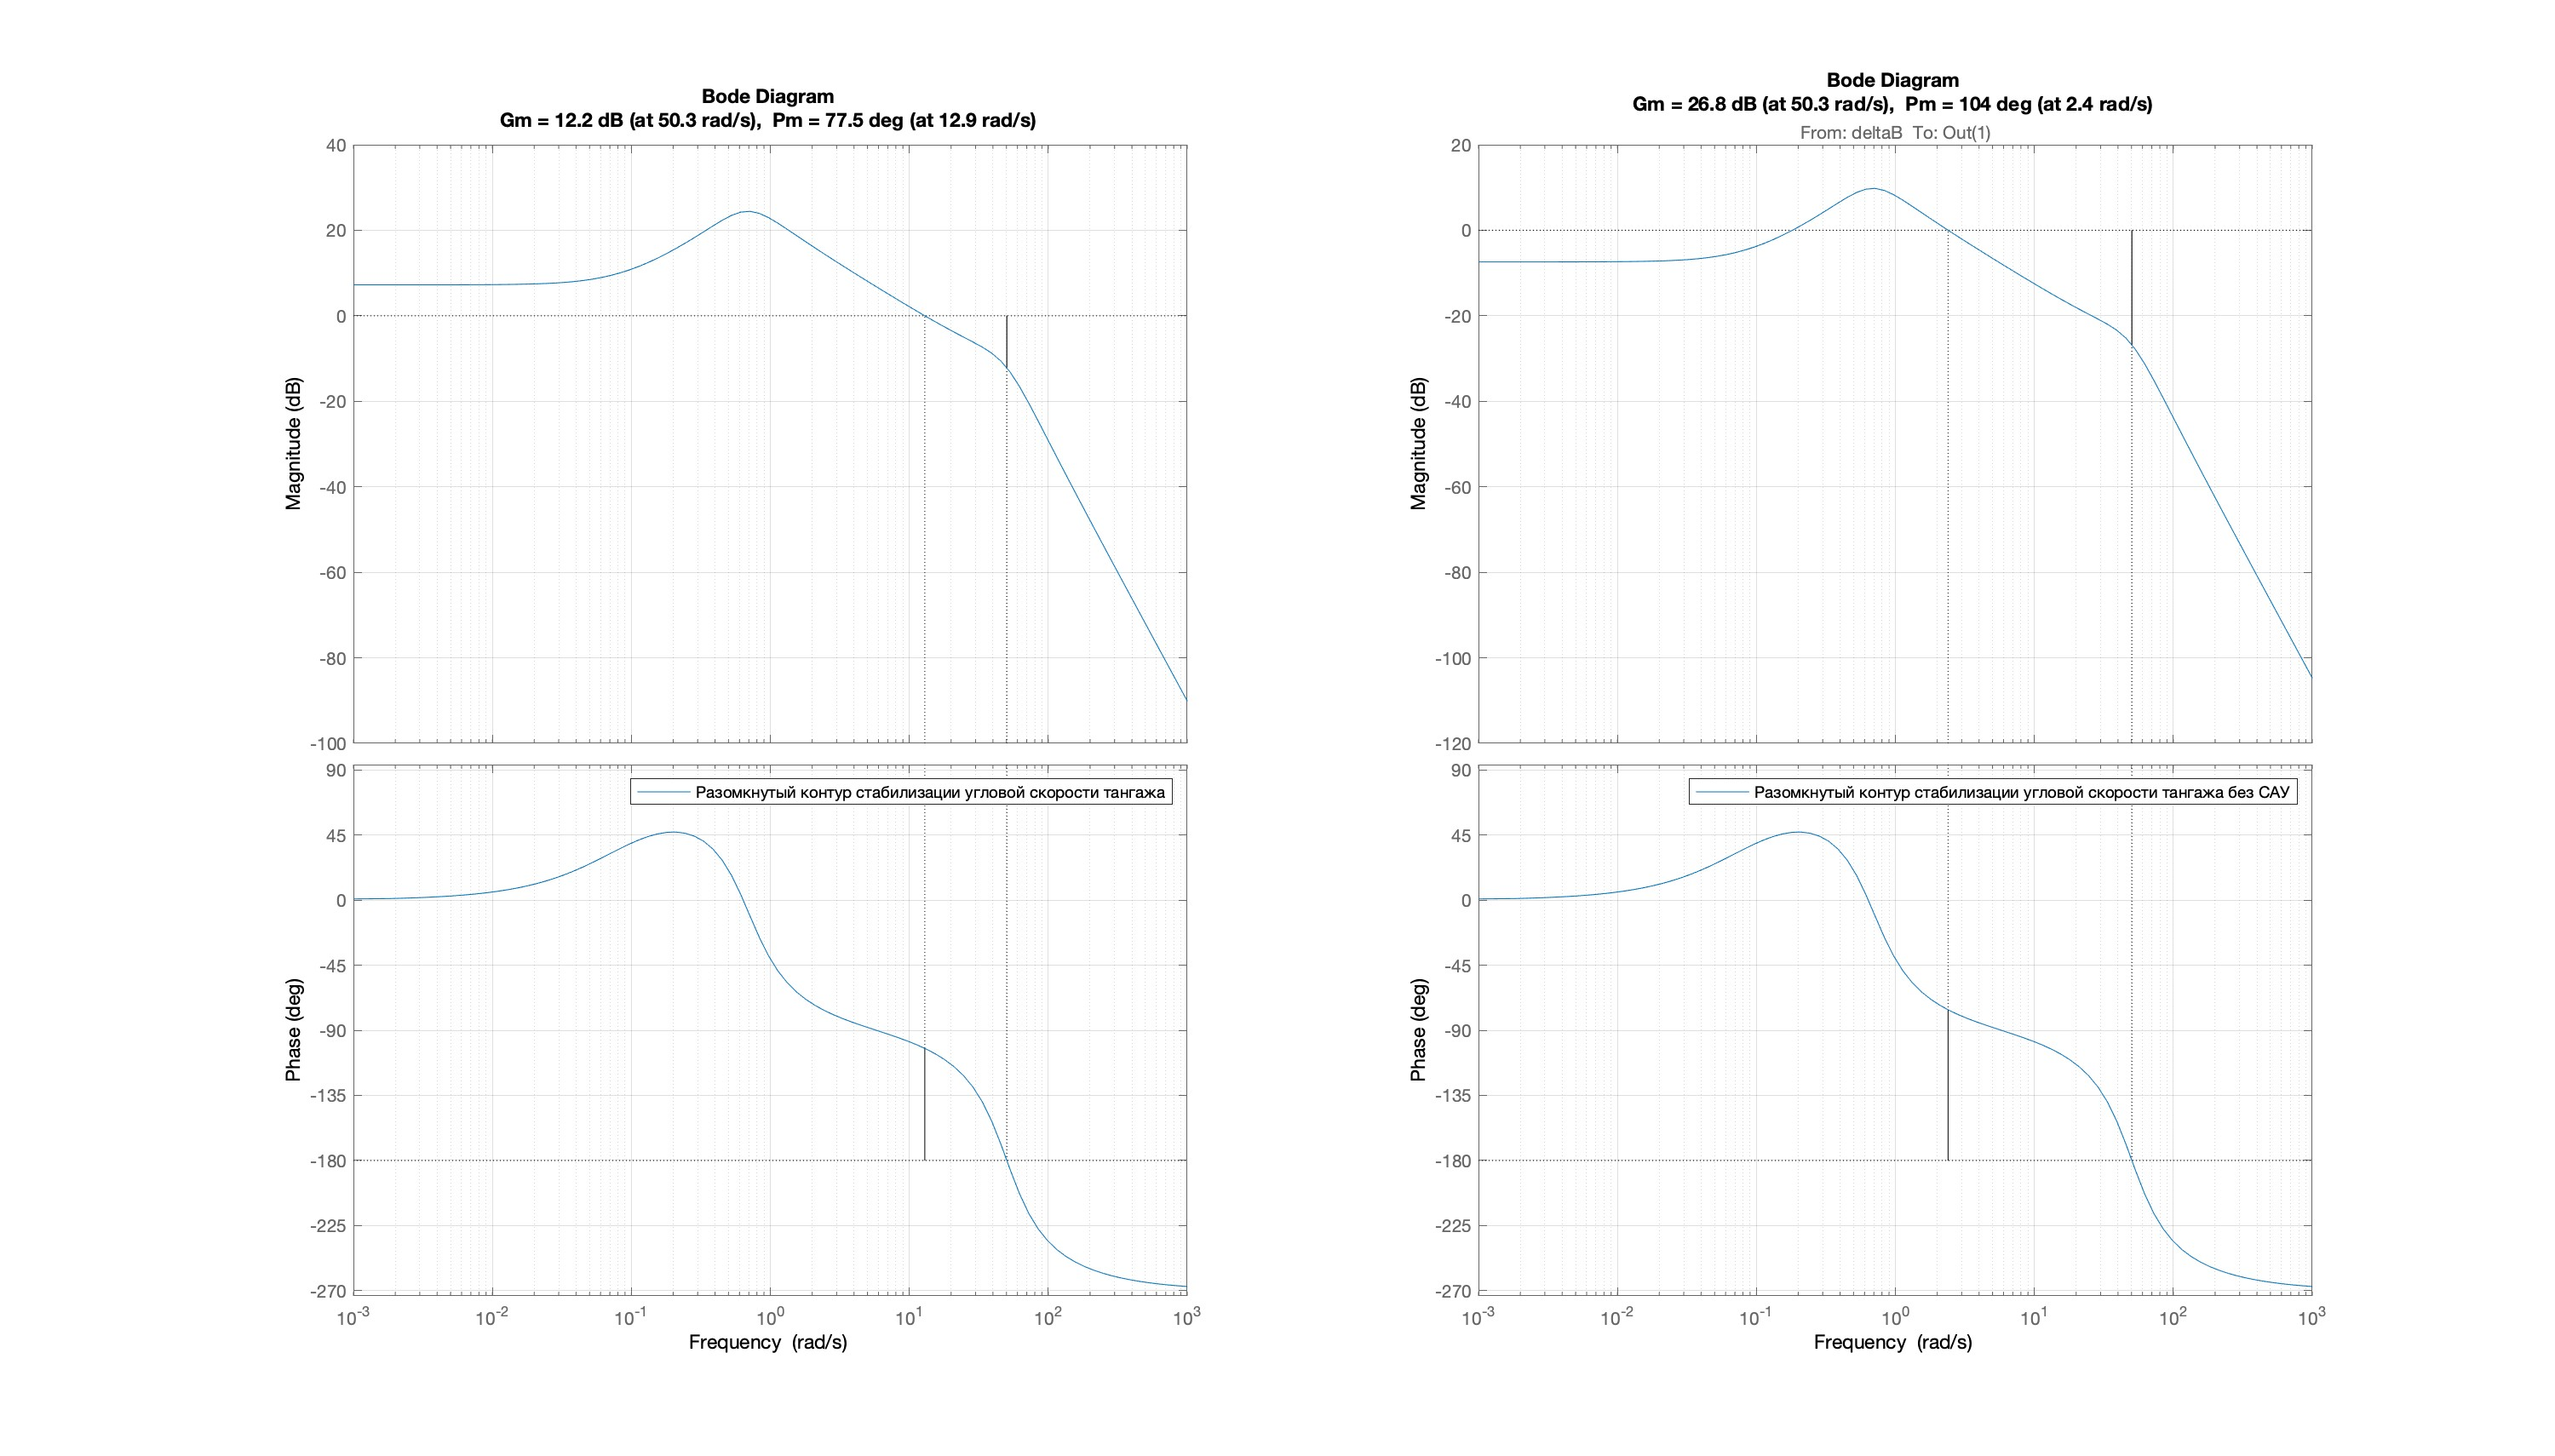
\includegraphics[width=\linewidth]{Оглавление/Part2/Sactions/Content/frequencies/Угловая скорость тангажа раз qKR.jpg}}
    \caption{ЛАФЧХ разомкнутого контура демпфирования угловой скорости тангажа}
    \label{fig:Угловая скорость тангажа раз qKR}
\end{figure}

Из рисунка \ref{fig:Угловая скорость тангажа раз qKR} видно, что до синтеза данного контура запасы устойчивости по амплитуде и по фазе не удовлетворяют заданным требованиям, то есть запас по амплитуде меньше 10 дб и запас по фазе меньше 45 град, а после синтеза $\Delta A = 12,3 $дБ $\Delta \varphi = 81^0$, следовательно, синтез проведен успешно, коэффициенты рассчитаны верно. Замкнутая система будет устойчива. Частота среза после синтеза не превысила граничного значения, она находится на участке с наклоном -20дб/дек, чего и требовалось достичь в результате синтеза.  

\begin{center}
    Контур стабилизации тангажа:
\end{center}

\begin{figure}[H]
    \center{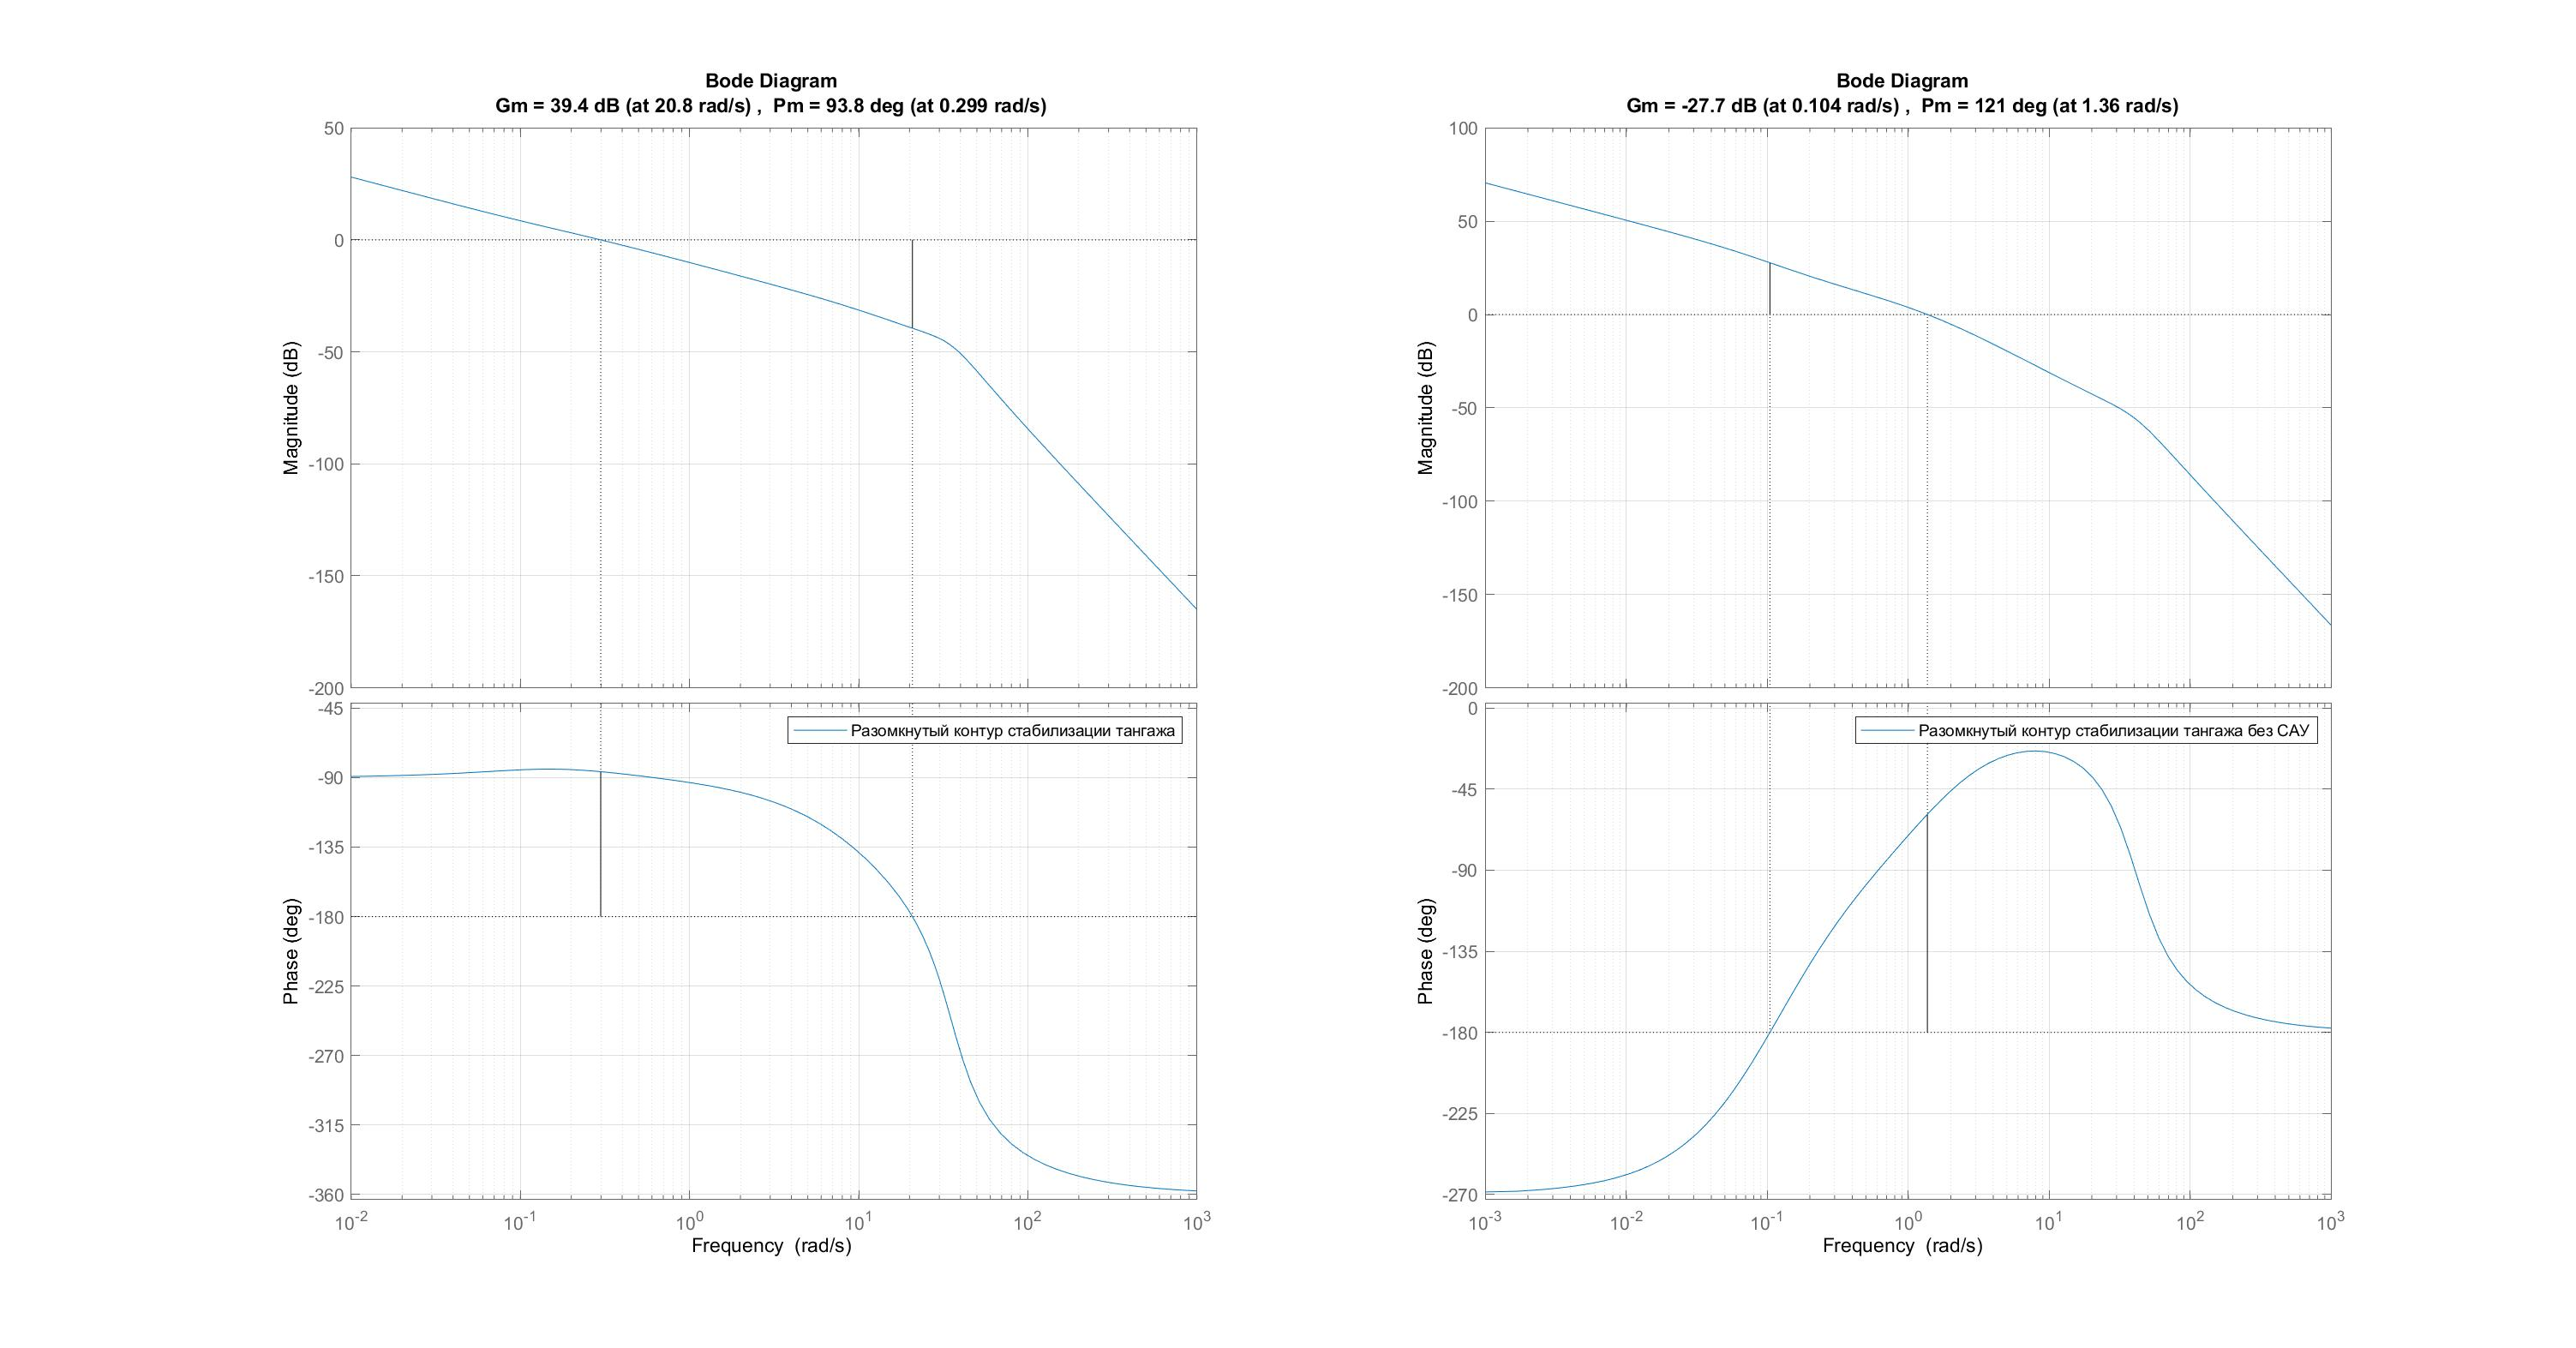
\includegraphics[width=\linewidth]{Оглавление/Part2/Sactions/Content/frequencies/Тангаж раз qKR.jpg}}
    \caption{ЛАФЧХ разомкнутого контура стабилизации тангажа}
    \label{fig:Тангаж раз qKR}
\end{figure}

Из рисунка \ref{fig:Тангаж раз qKR} видно, что до синтеза данного контура запасы устойчивости по амплитуде и по фазе не удовлетворяют заданным требованиям, то есть запас по амплитуде меньше 10 дб и запас по фазе меньше 45 град, а после синтеза $\Delta A = 39,4 $дБ $\Delta \varphi = 94^0$, следовательно, синтез проведен успешно, коэффициенты рассчитаны верно. Замкнутая система будет устойчива.  

\begin{center}
    Контур вертикальной скорости:
\end{center}

\begin{figure}[H]
    \center{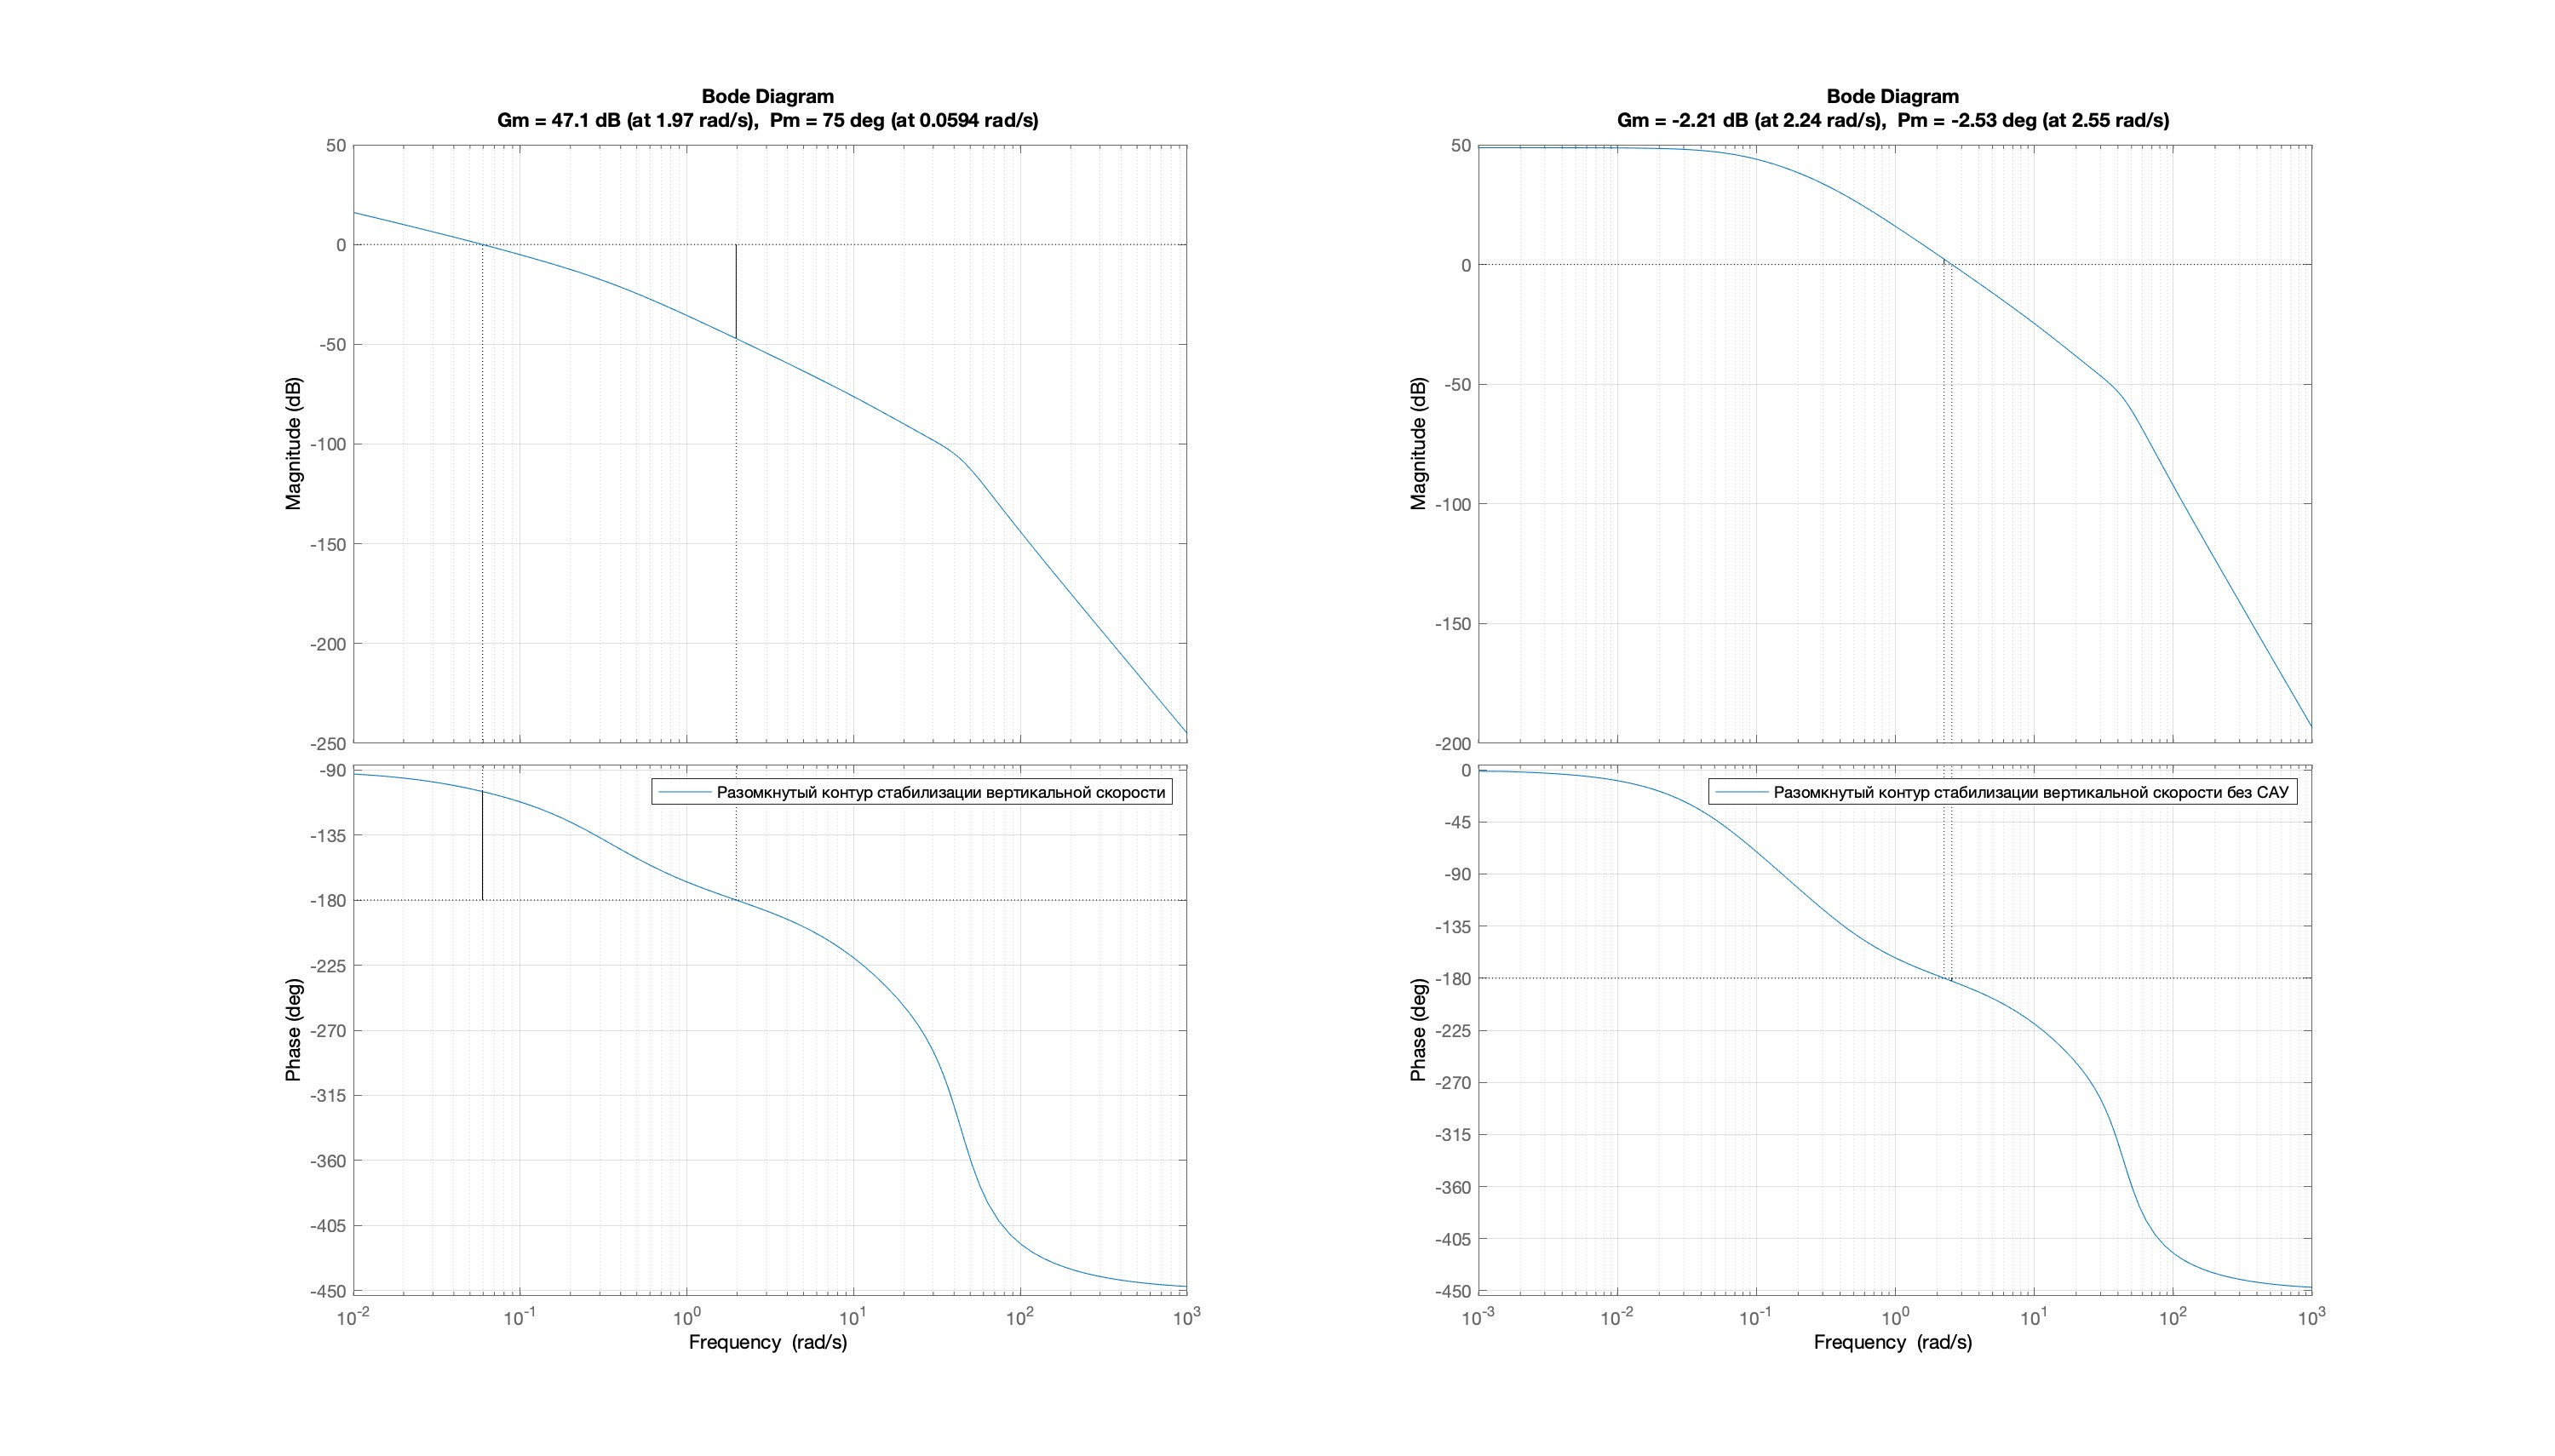
\includegraphics[width=\linewidth]{Оглавление/Part2/Sactions/Content/frequencies/Вертикальная скорость раз qKR.jpg}}
    \caption{ЛАФЧХ разомкнутого контура стабилизации вертикальной скорости}
    \label{fig:Вертикальная скорость раз qKR}
\end{figure}

Из рисунка \ref{fig:Вертикальная скорость раз qKR} видно, что после синтеза $\Delta A = 41,9 $дБ $\Delta \varphi = 72^0$, следовательно, синтез проведен успешно, коэффициенты рассчитаны верно. Замкнутая система будет устойчива.  

\begin{figure}[H]
    \center{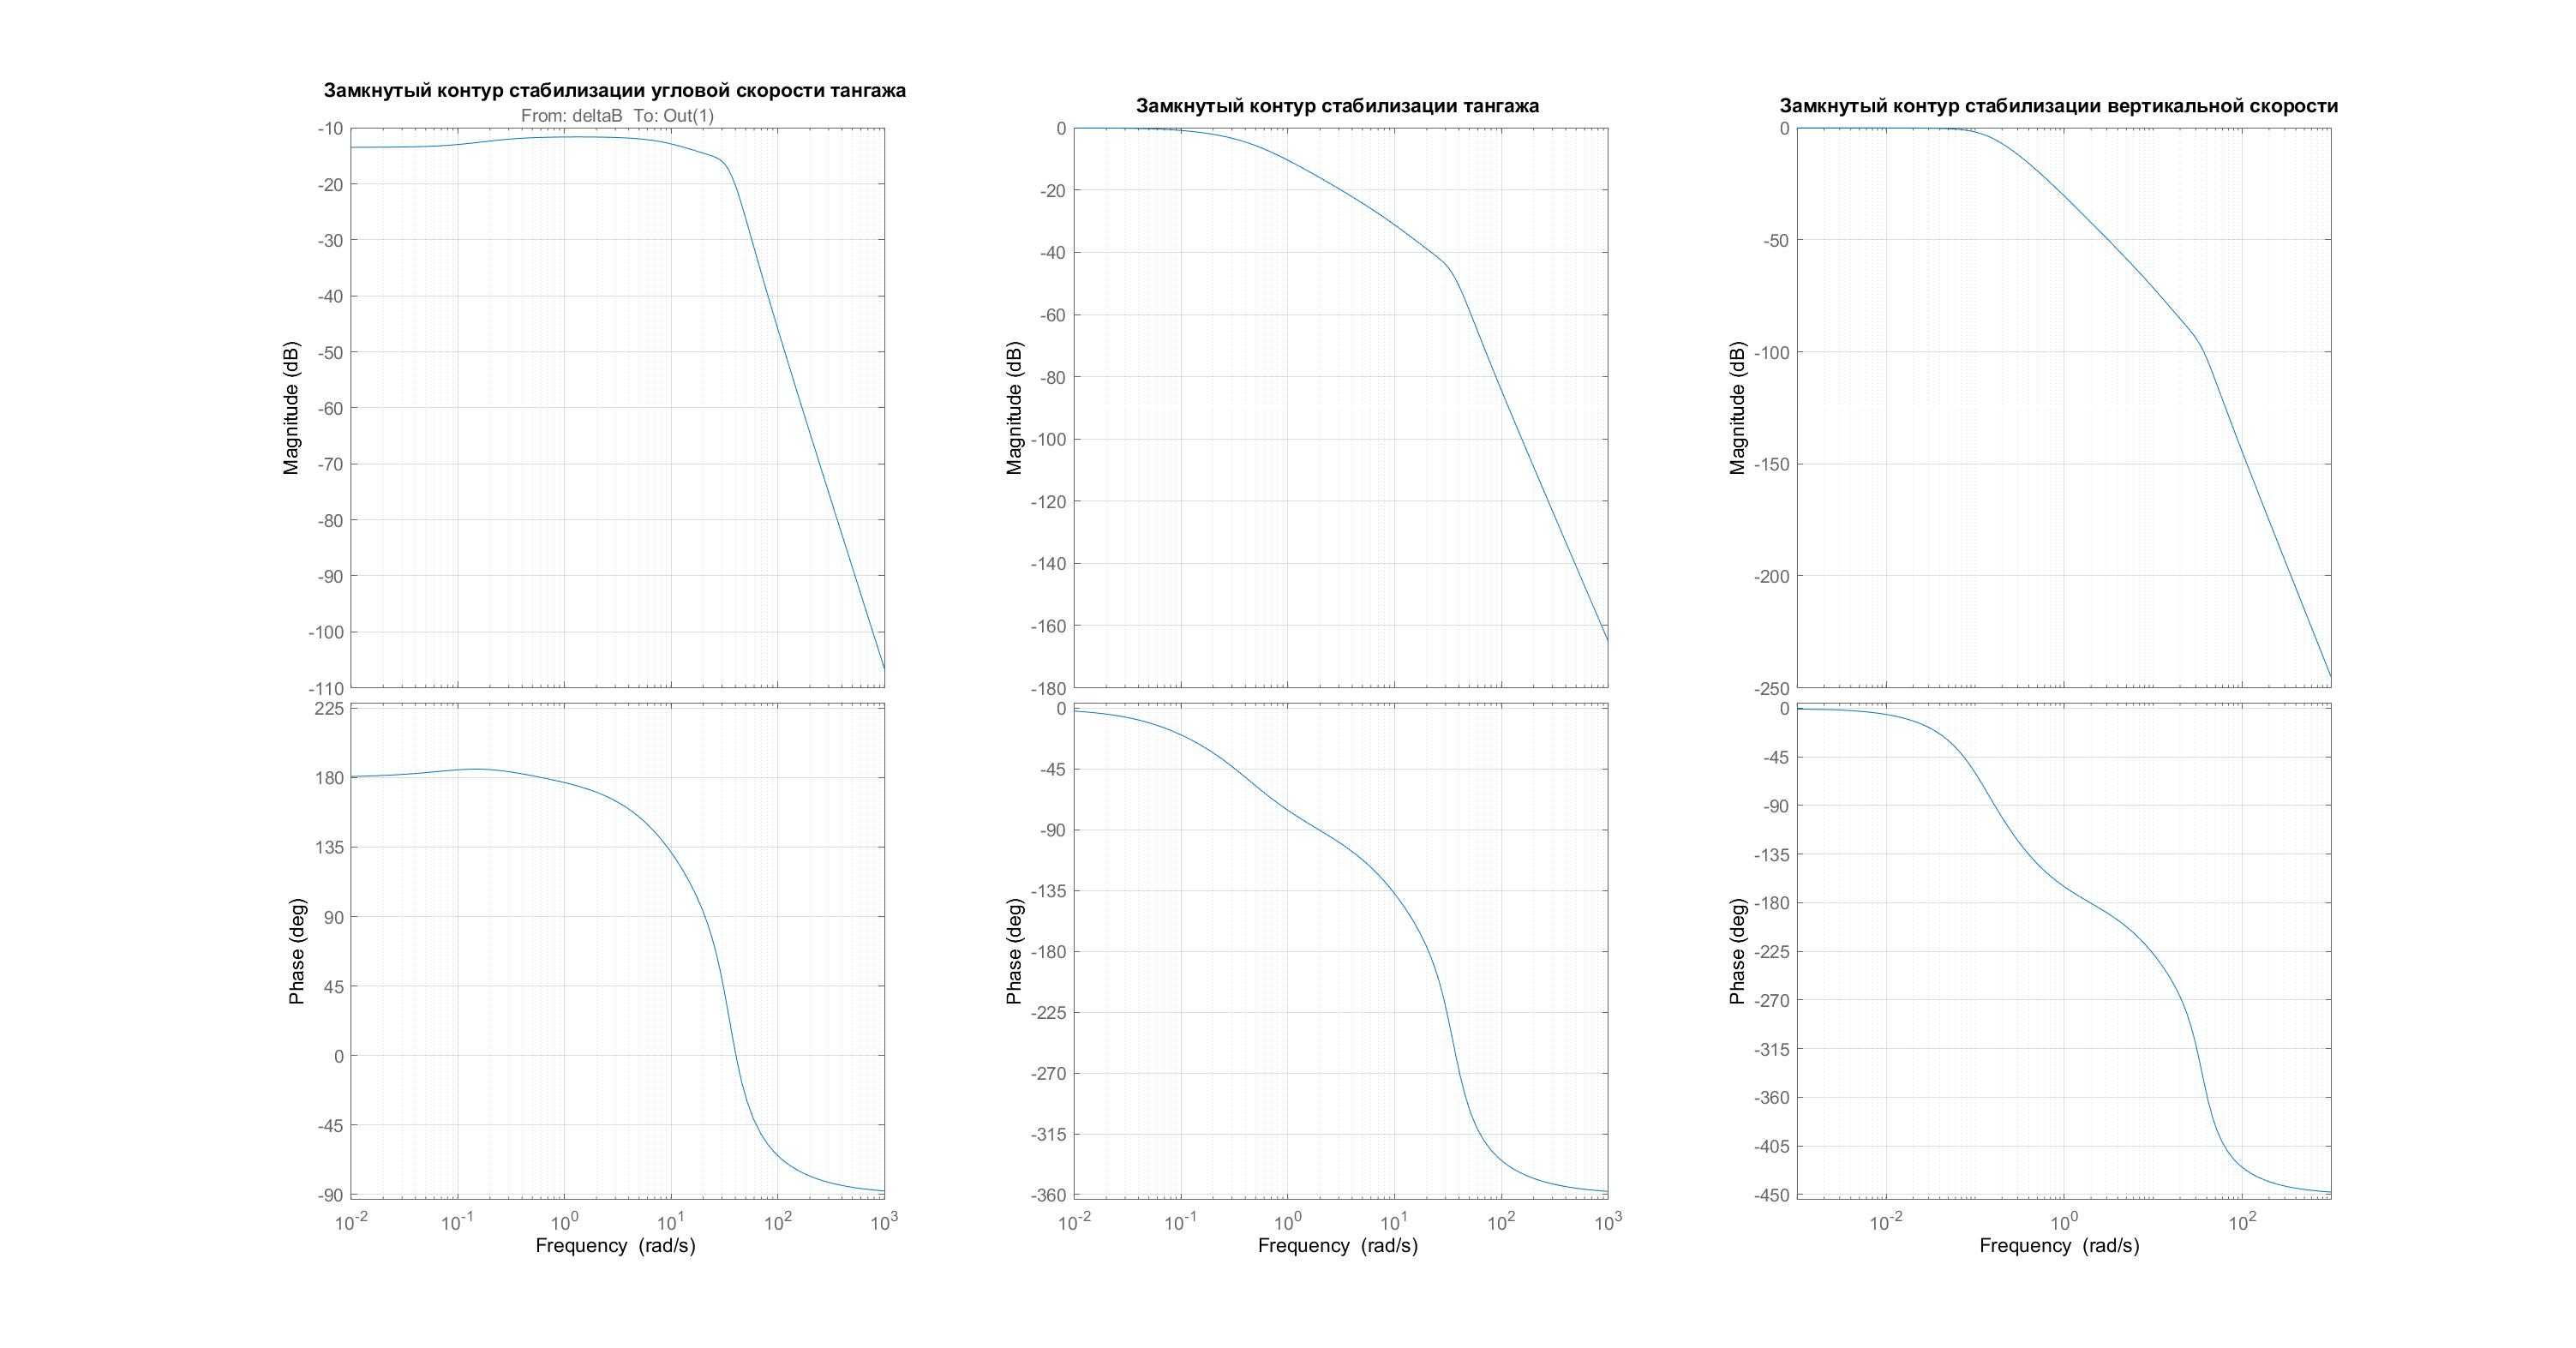
\includegraphics[width=\linewidth]{Оглавление/Part2/Sactions/Content/frequencies/ZAM qKR.jpg}}
    \caption{ЛАФЧХ замкнутого контура }
    \label{fig:Вертикальная скорость зам qKR}
\end{figure}

\subsection{Нелинейное моделирование САУ}

В данном разделе проводится анализ линейной и нелинейной САУ. В Simulink реализуется система управления на крейсерском режиме полета. Крейсерскому режиму полета для самолета-прототипа Concorde соответствуют М=0,7521 и Н=10 км. Найденные коэффициенты для данного режима полета приведены в таблице 2.9 раздела 2. 

В системе появляется нелинейность из-за введения ограничений по углу тангажа, скорости изменения сигнала, поступающего на привод и т.д. В Simulink ограничения можно ввести при помощи блоков «Saturation» и «Rate limiter». Величины ограничений приведены в таблице \ref{tab:Нелинейности}

\begin{table}[H]
    \centering
    \caption{ограничения, вводимые в САУ}
    \begin{tabular}{|c|c|c|c|c|}
    \hline
        № & Параметр & Обозначение & Значение & Единица измерения \\ \hline
        1 & Максимальный угол & $\delta_\text{э}_\text{макс}$ & $\pm 25$ & град \\ 
         & отклонения элевонов &  &  & \\ \hline
        2 & Максимальный угол & $\vartheta_\text{макс}$ & $\pm 23$ & град\\
         & тангажа &  &  & \\ \hline
         & Скорость изменения &  &  & \\ 
        3 & сигнала на & $\dot{\sigma_n}$ & $\pm 30$ &ед \\ 
        & выходе в привод &  &  & \\ \hline
        4 & Величина входного &  &  & \\ 
         & сигнала привода & $\sigma_n$ & $\pm 15$ &ед \\ \hline
    \end{tabular}
    \label{tab:Нелинейности}
\end{table}

Моделирование нелинейной системы проводится при стабилизации вертикальной скорости $V_y = 10$м/с, моделирование линейной при стабилизации угла курса  .Результаты линейного и нелинейного моделирования представлены в виде графиков различных переходных процессов (см. рис.3.1-3.18). Схема системы представлена в конце данного раздела.

\begin{center}
    \subsubsection{Моделирование линейной и нелинейной САУ}Моделирование линейной и нелинейной САУ
\end{center}

Структурные схемы линейной и нелинейной системы представлены в приложениях.

\begin{figure}[H]
    \center{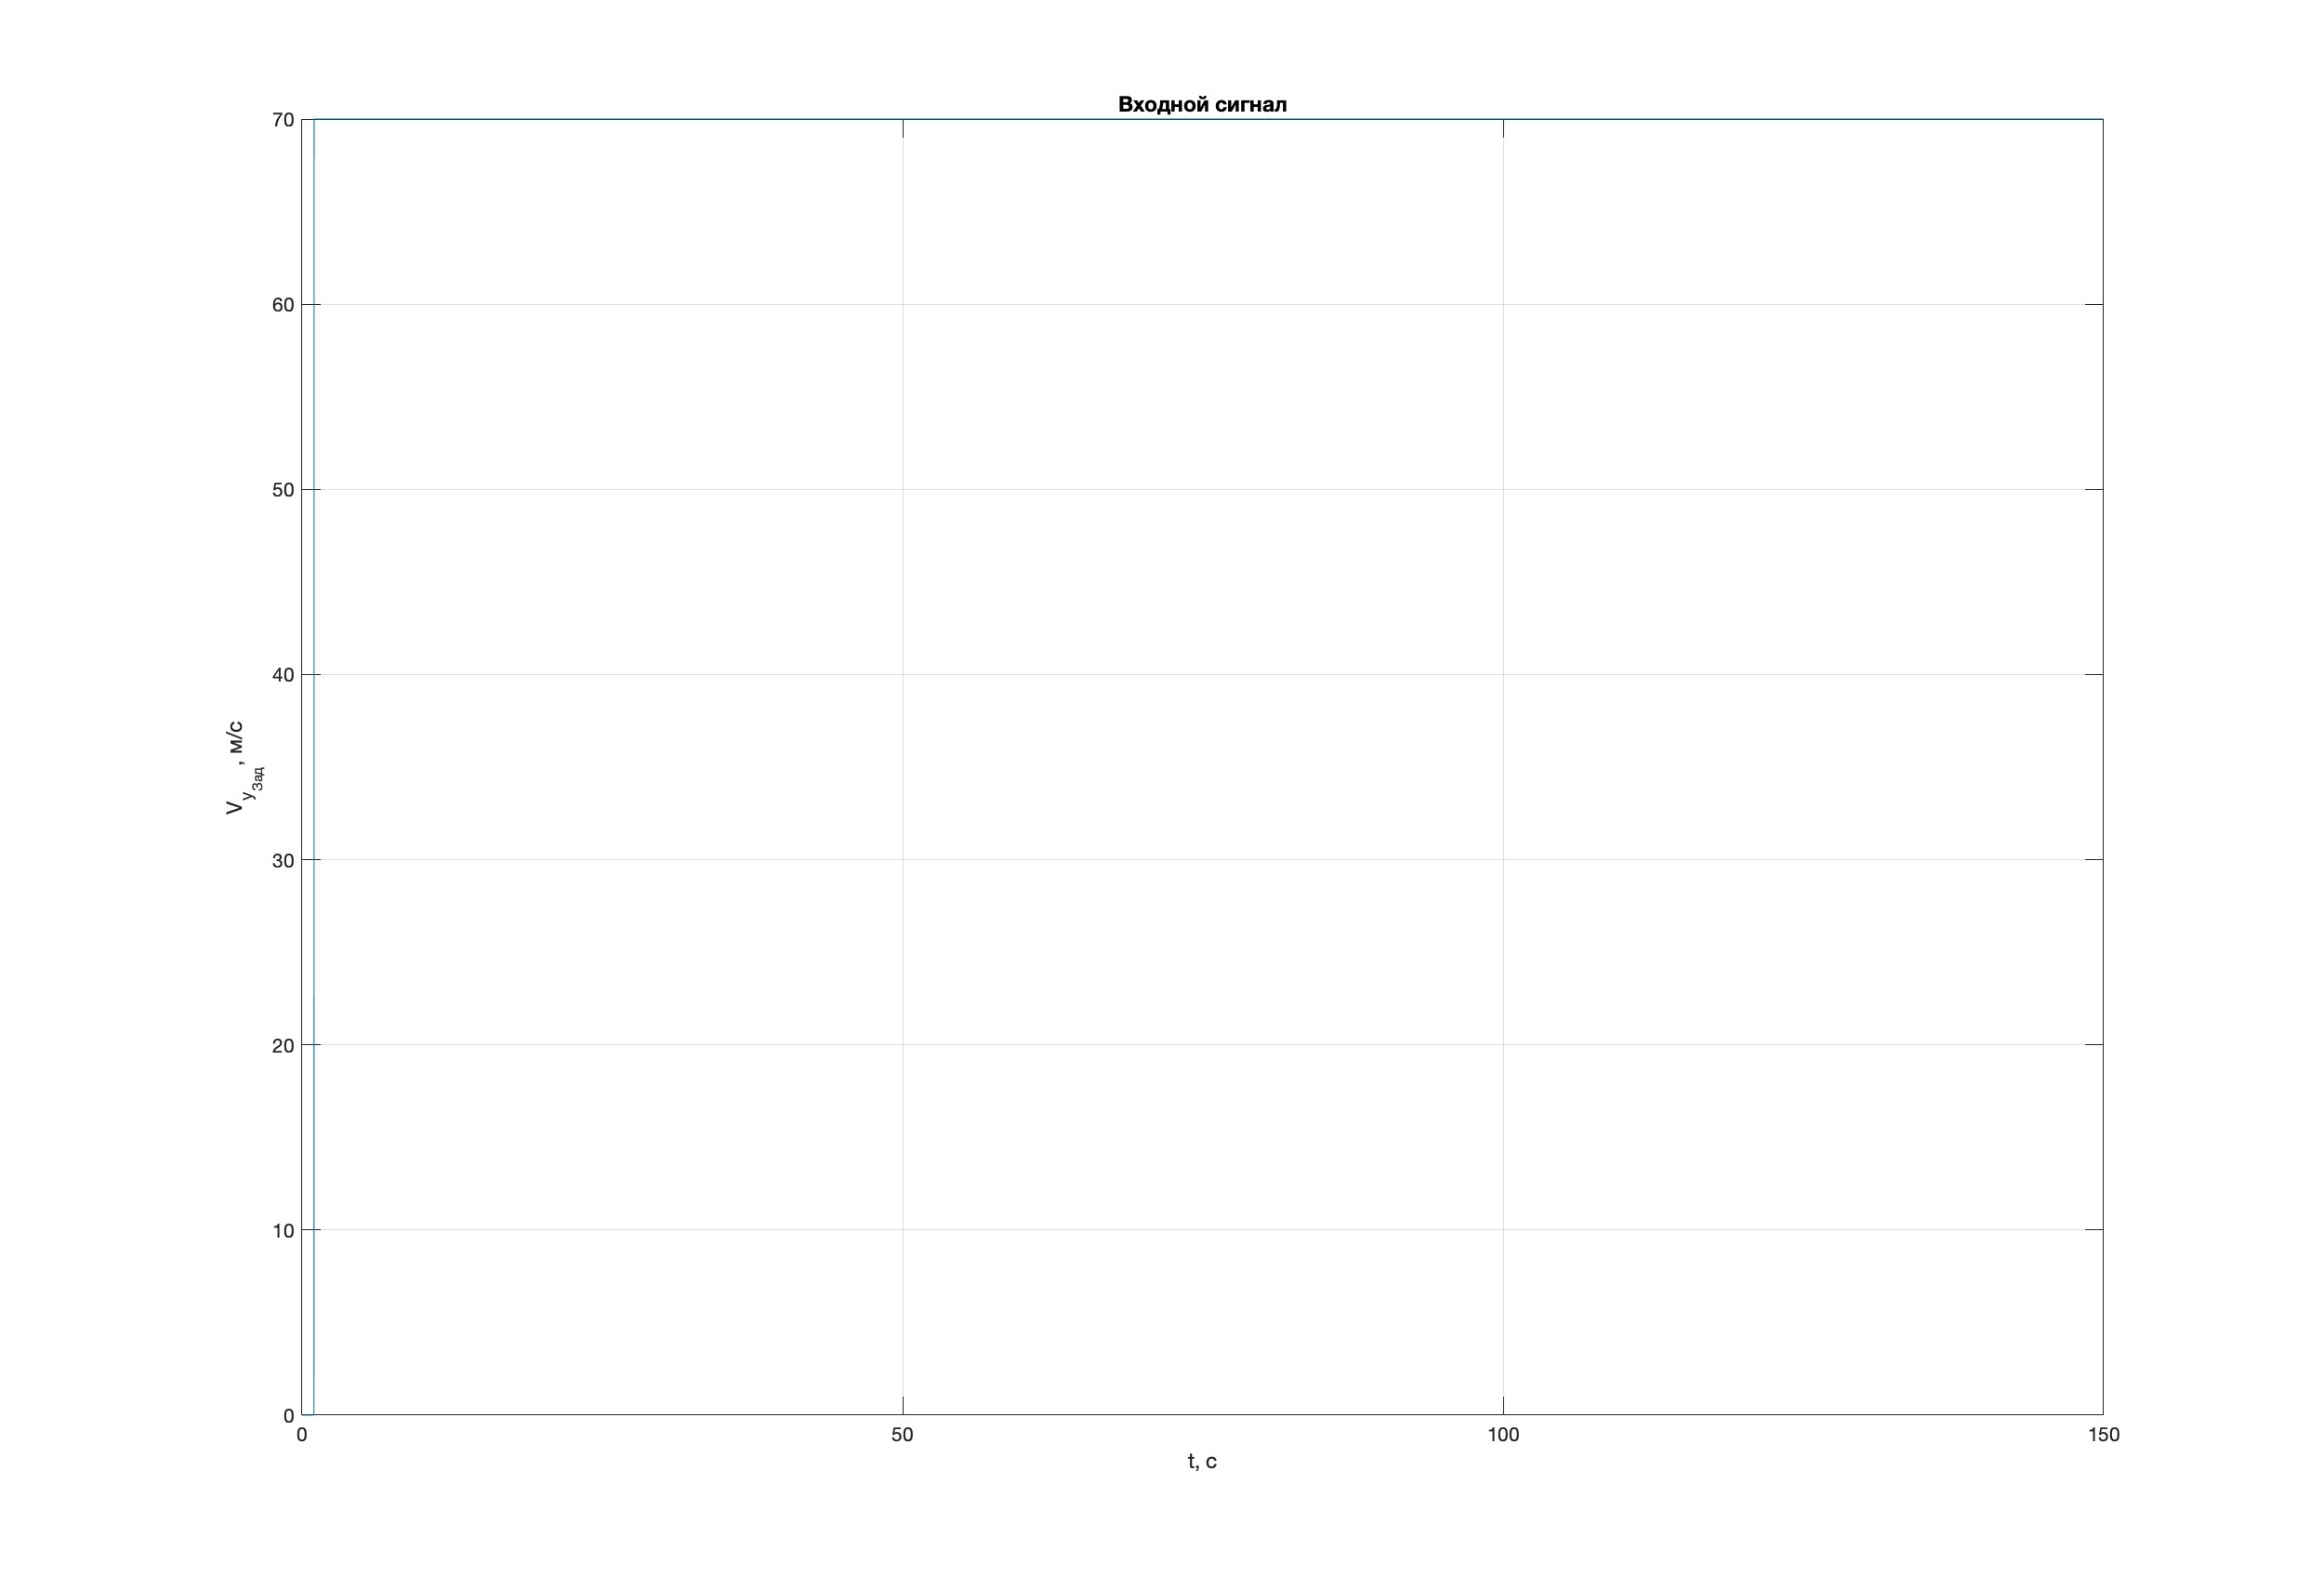
\includegraphics[width=\linewidth]{Оглавление/Part2/Sactions/Content/NotLinFig/Линейный ВС.jpg}}
    \caption{Входной сигнал системы стабилизации вертикальной скорости }
    \label{fig:Входной сигнал системы стабилизации вертикальной скорости}
\end{figure}

\begin{figure}[H]
    \center{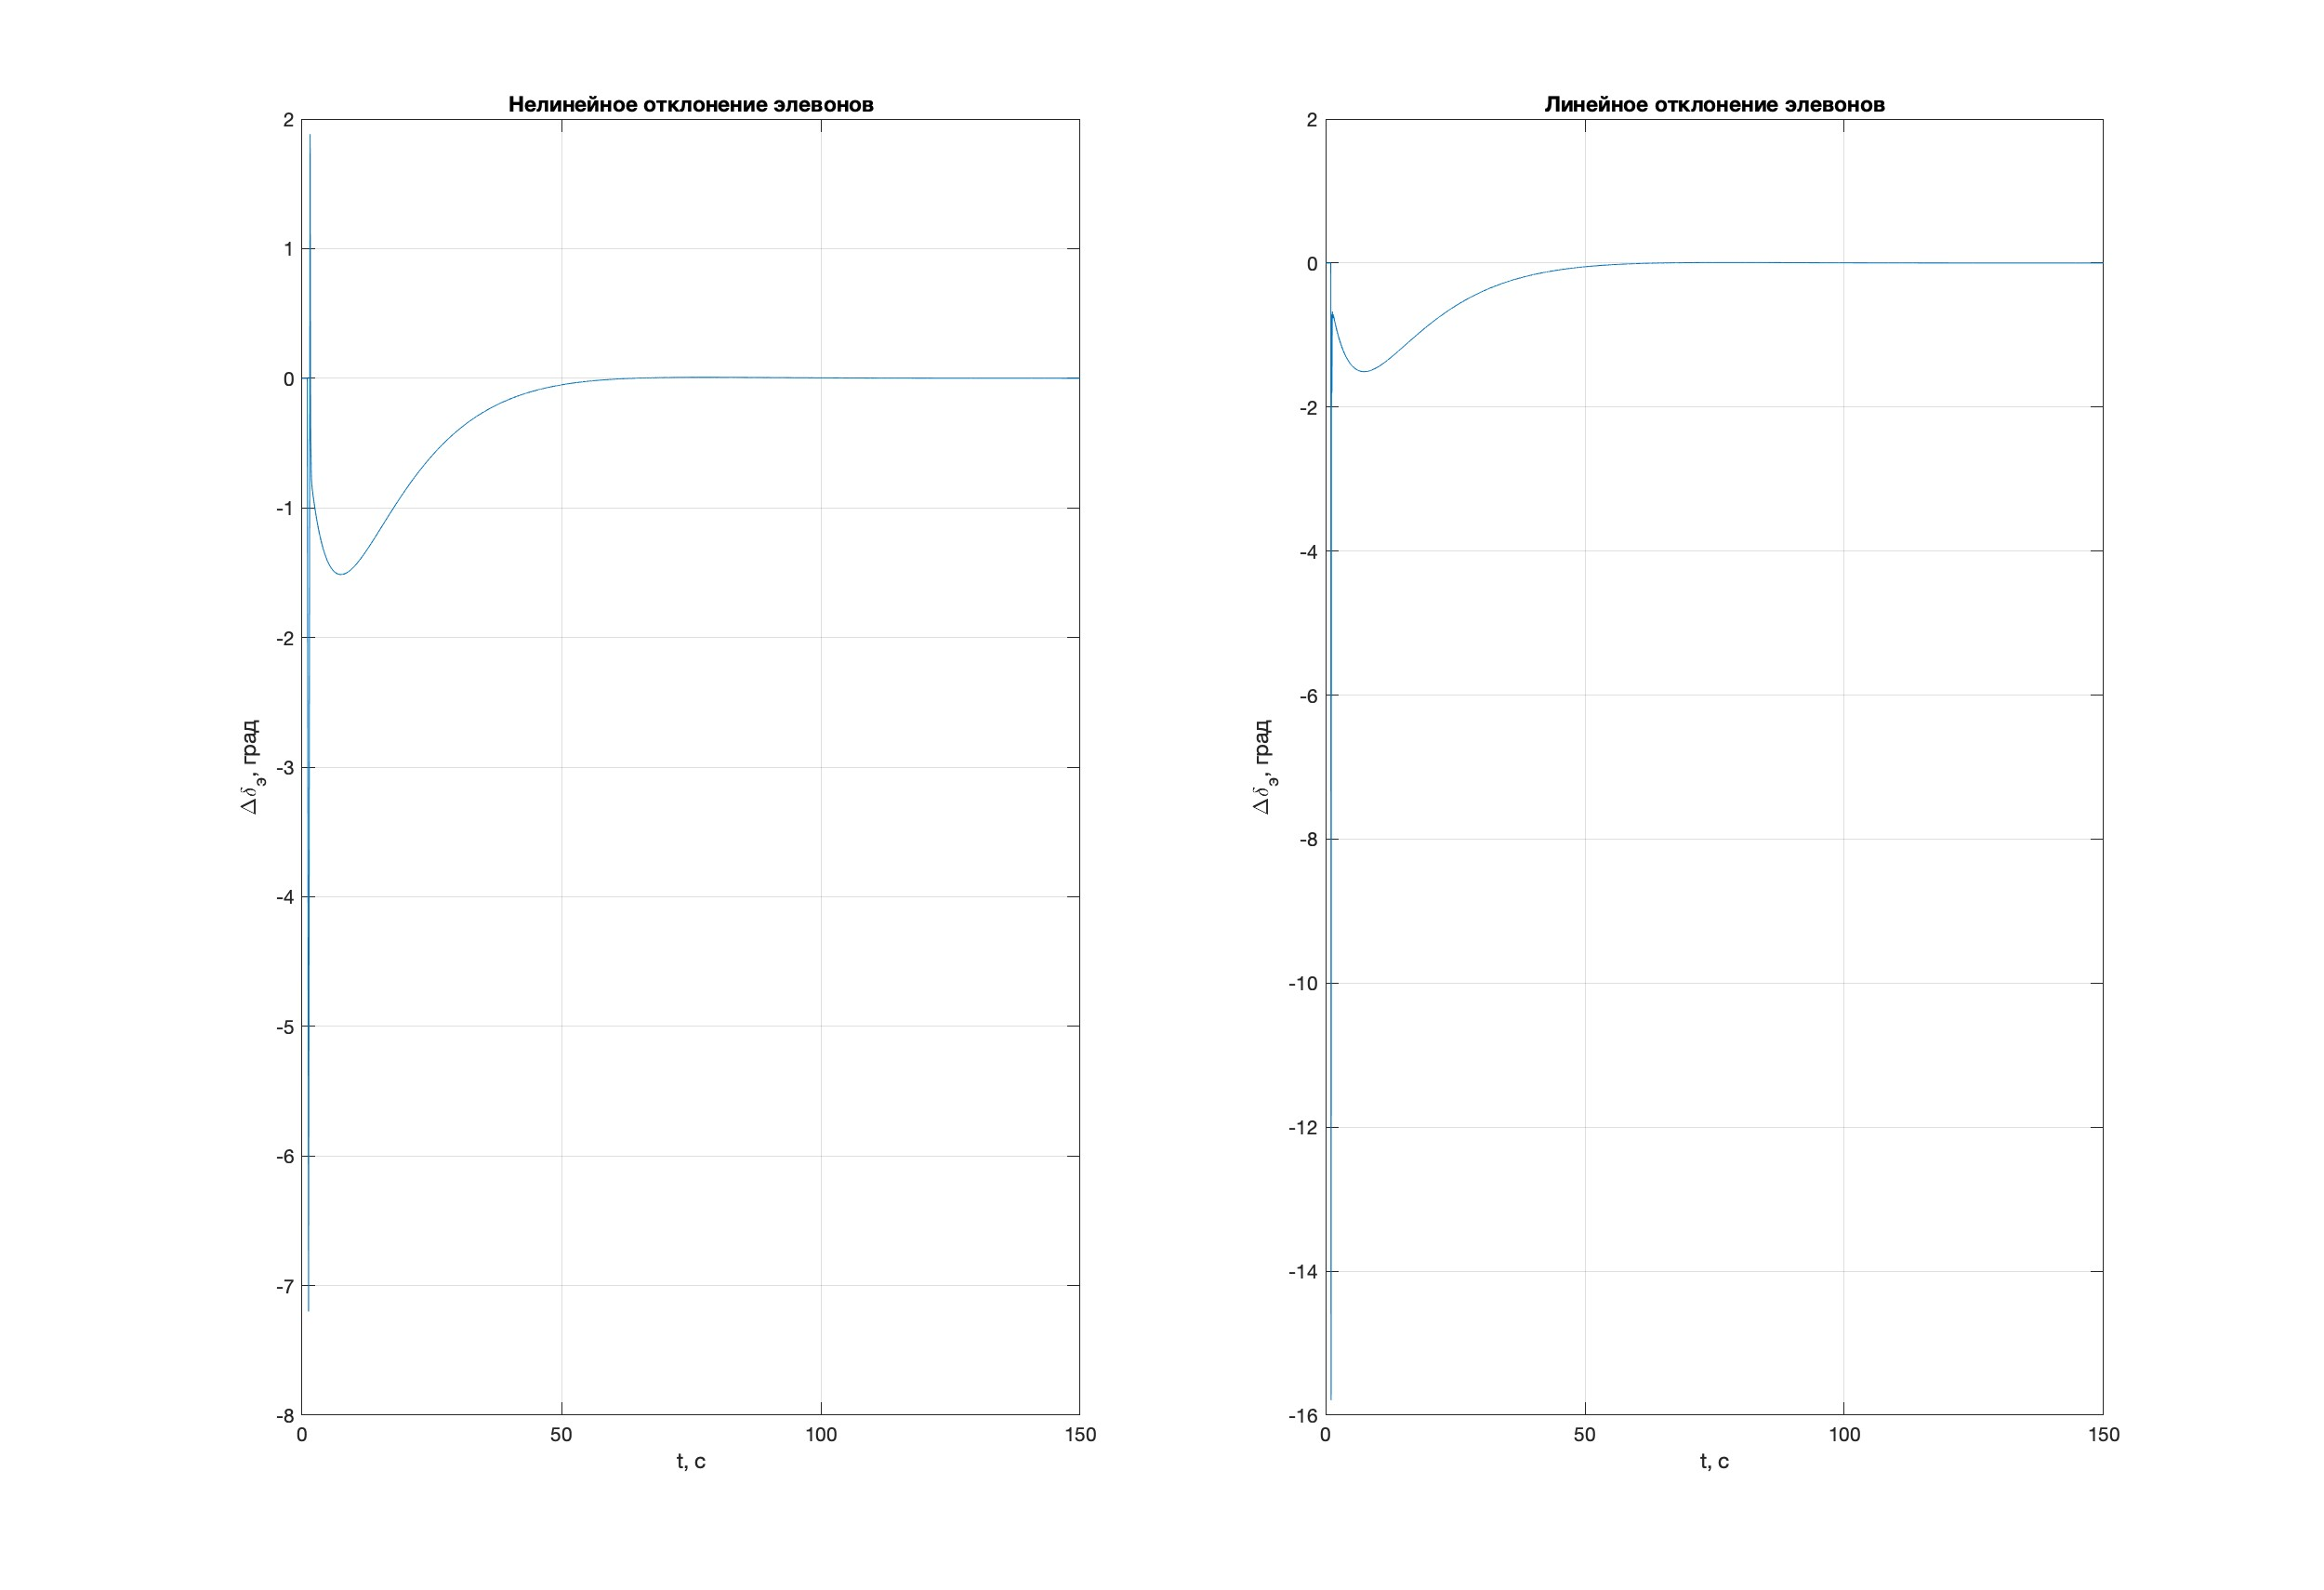
\includegraphics[width=\linewidth]{Оглавление/Part2/Sactions/Content/NotLinFig/Руль.jpg}}
    \caption{Отклонения элевонов для стабилизации угла скольжения}
    \label{fig:Отклонения элевонов для стабилизации угла скольжения}
\end{figure}

\begin{figure}[H]
    \center{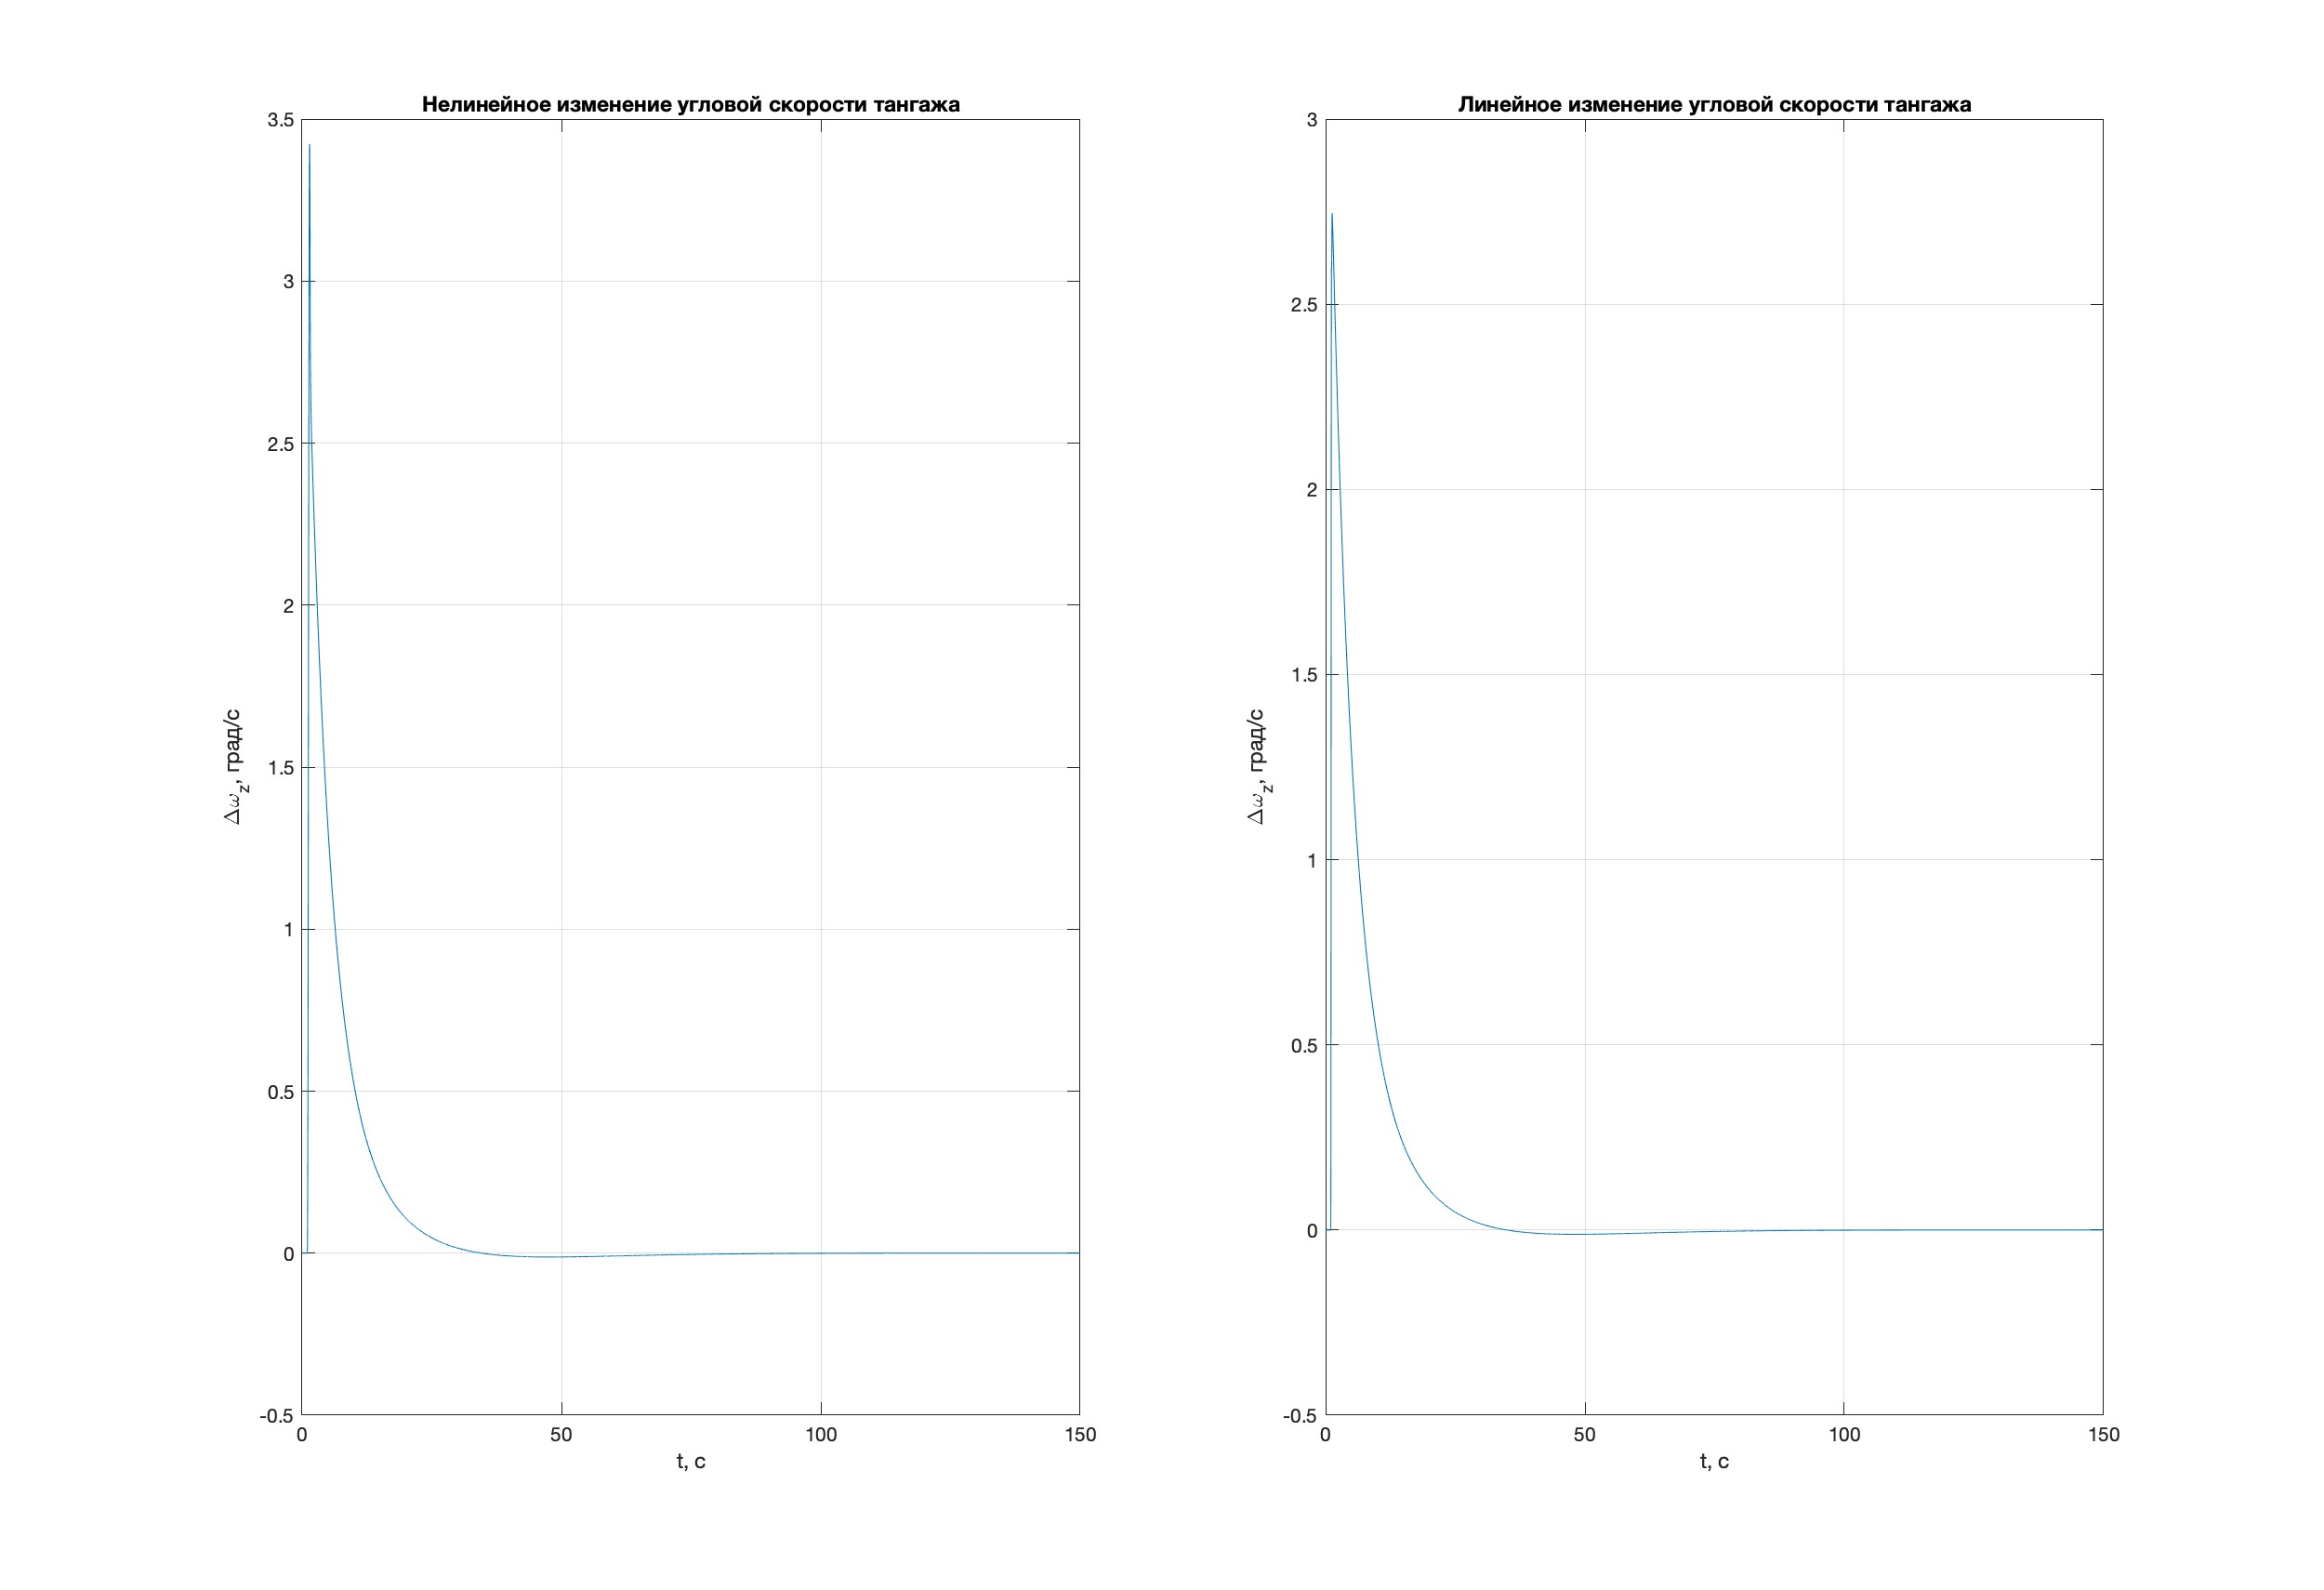
\includegraphics[width=\linewidth]{Оглавление/Part2/Sactions/Content/NotLinFig/wz.jpg}}
    \caption{Изменение угловой скорости тангажа в процессе стабилизации вертикальной скорости}
    \label{fig:Изменение угловой скорости тангажа в процессе стабилизации вертикальной скорости}
\end{figure}

\begin{figure}[H]
    \center{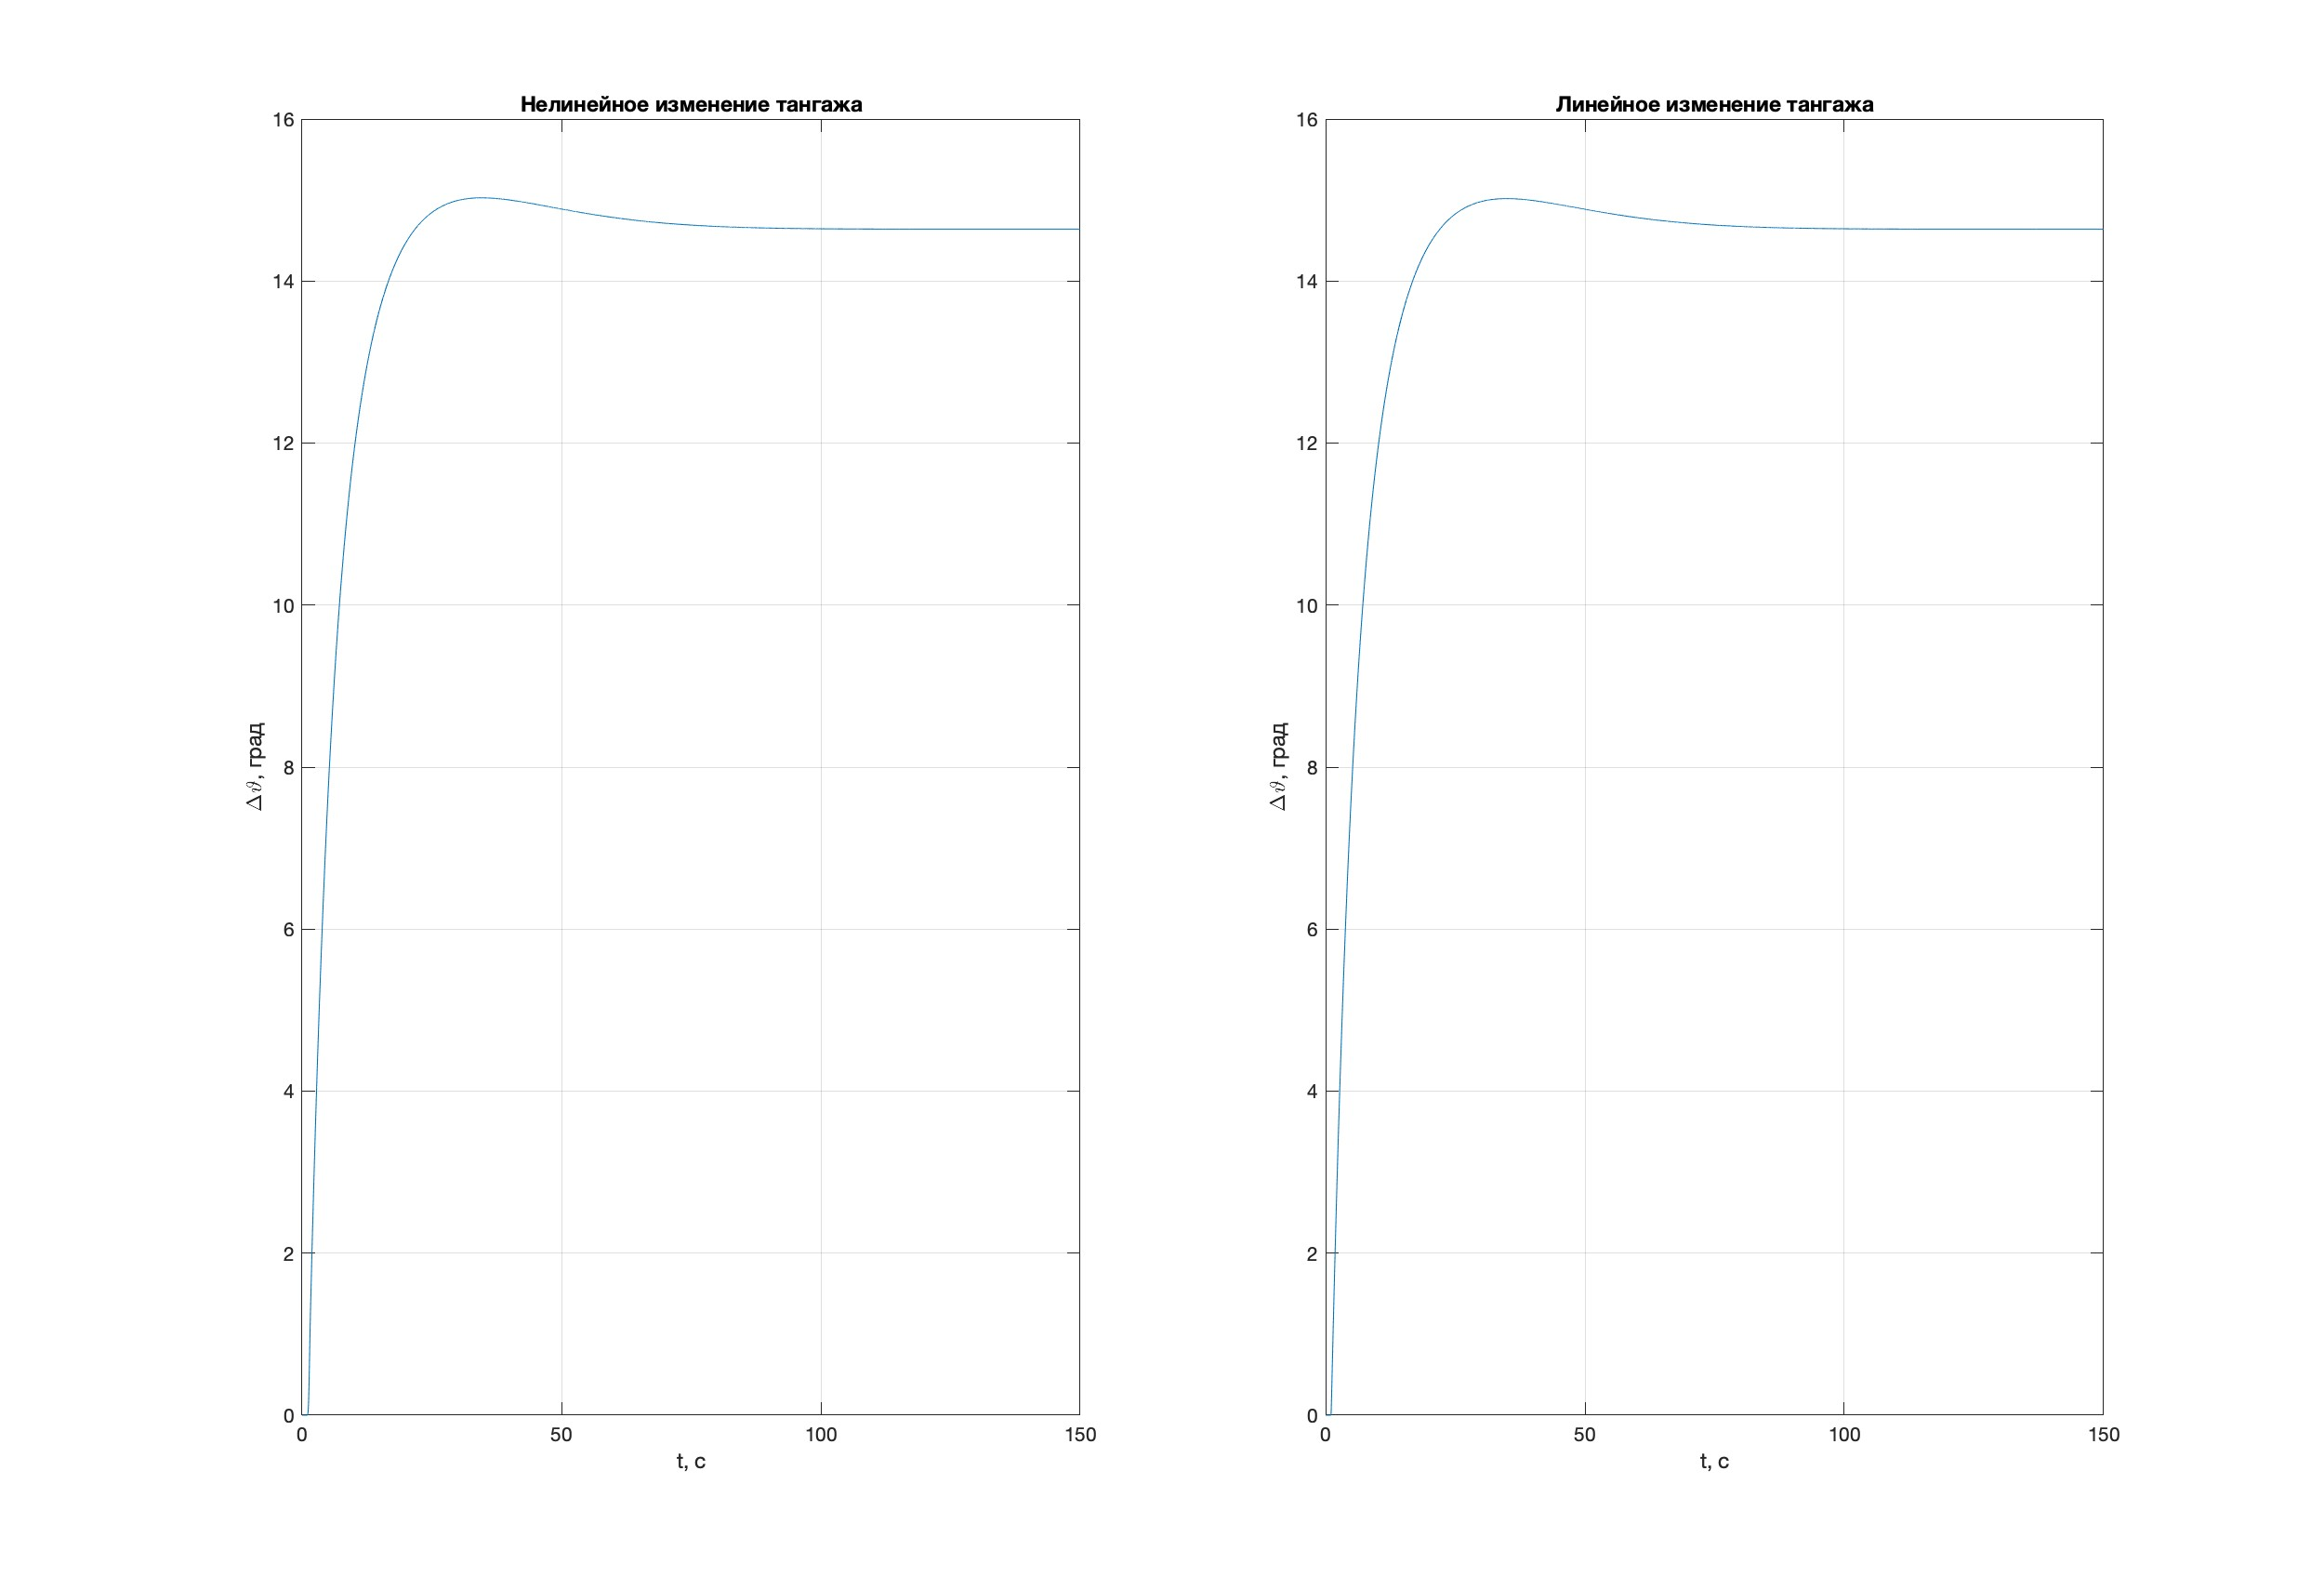
\includegraphics[width=\linewidth]{Оглавление/Part2/Sactions/Content/NotLinFig/vartheta.jpg}}
    \caption{Изменение угла тангажа при стабилизации вертикальной скорости}
    \label{fig:Входной сигнал системы изменения тангажа}
\end{figure}

\begin{figure}[H]
    \center{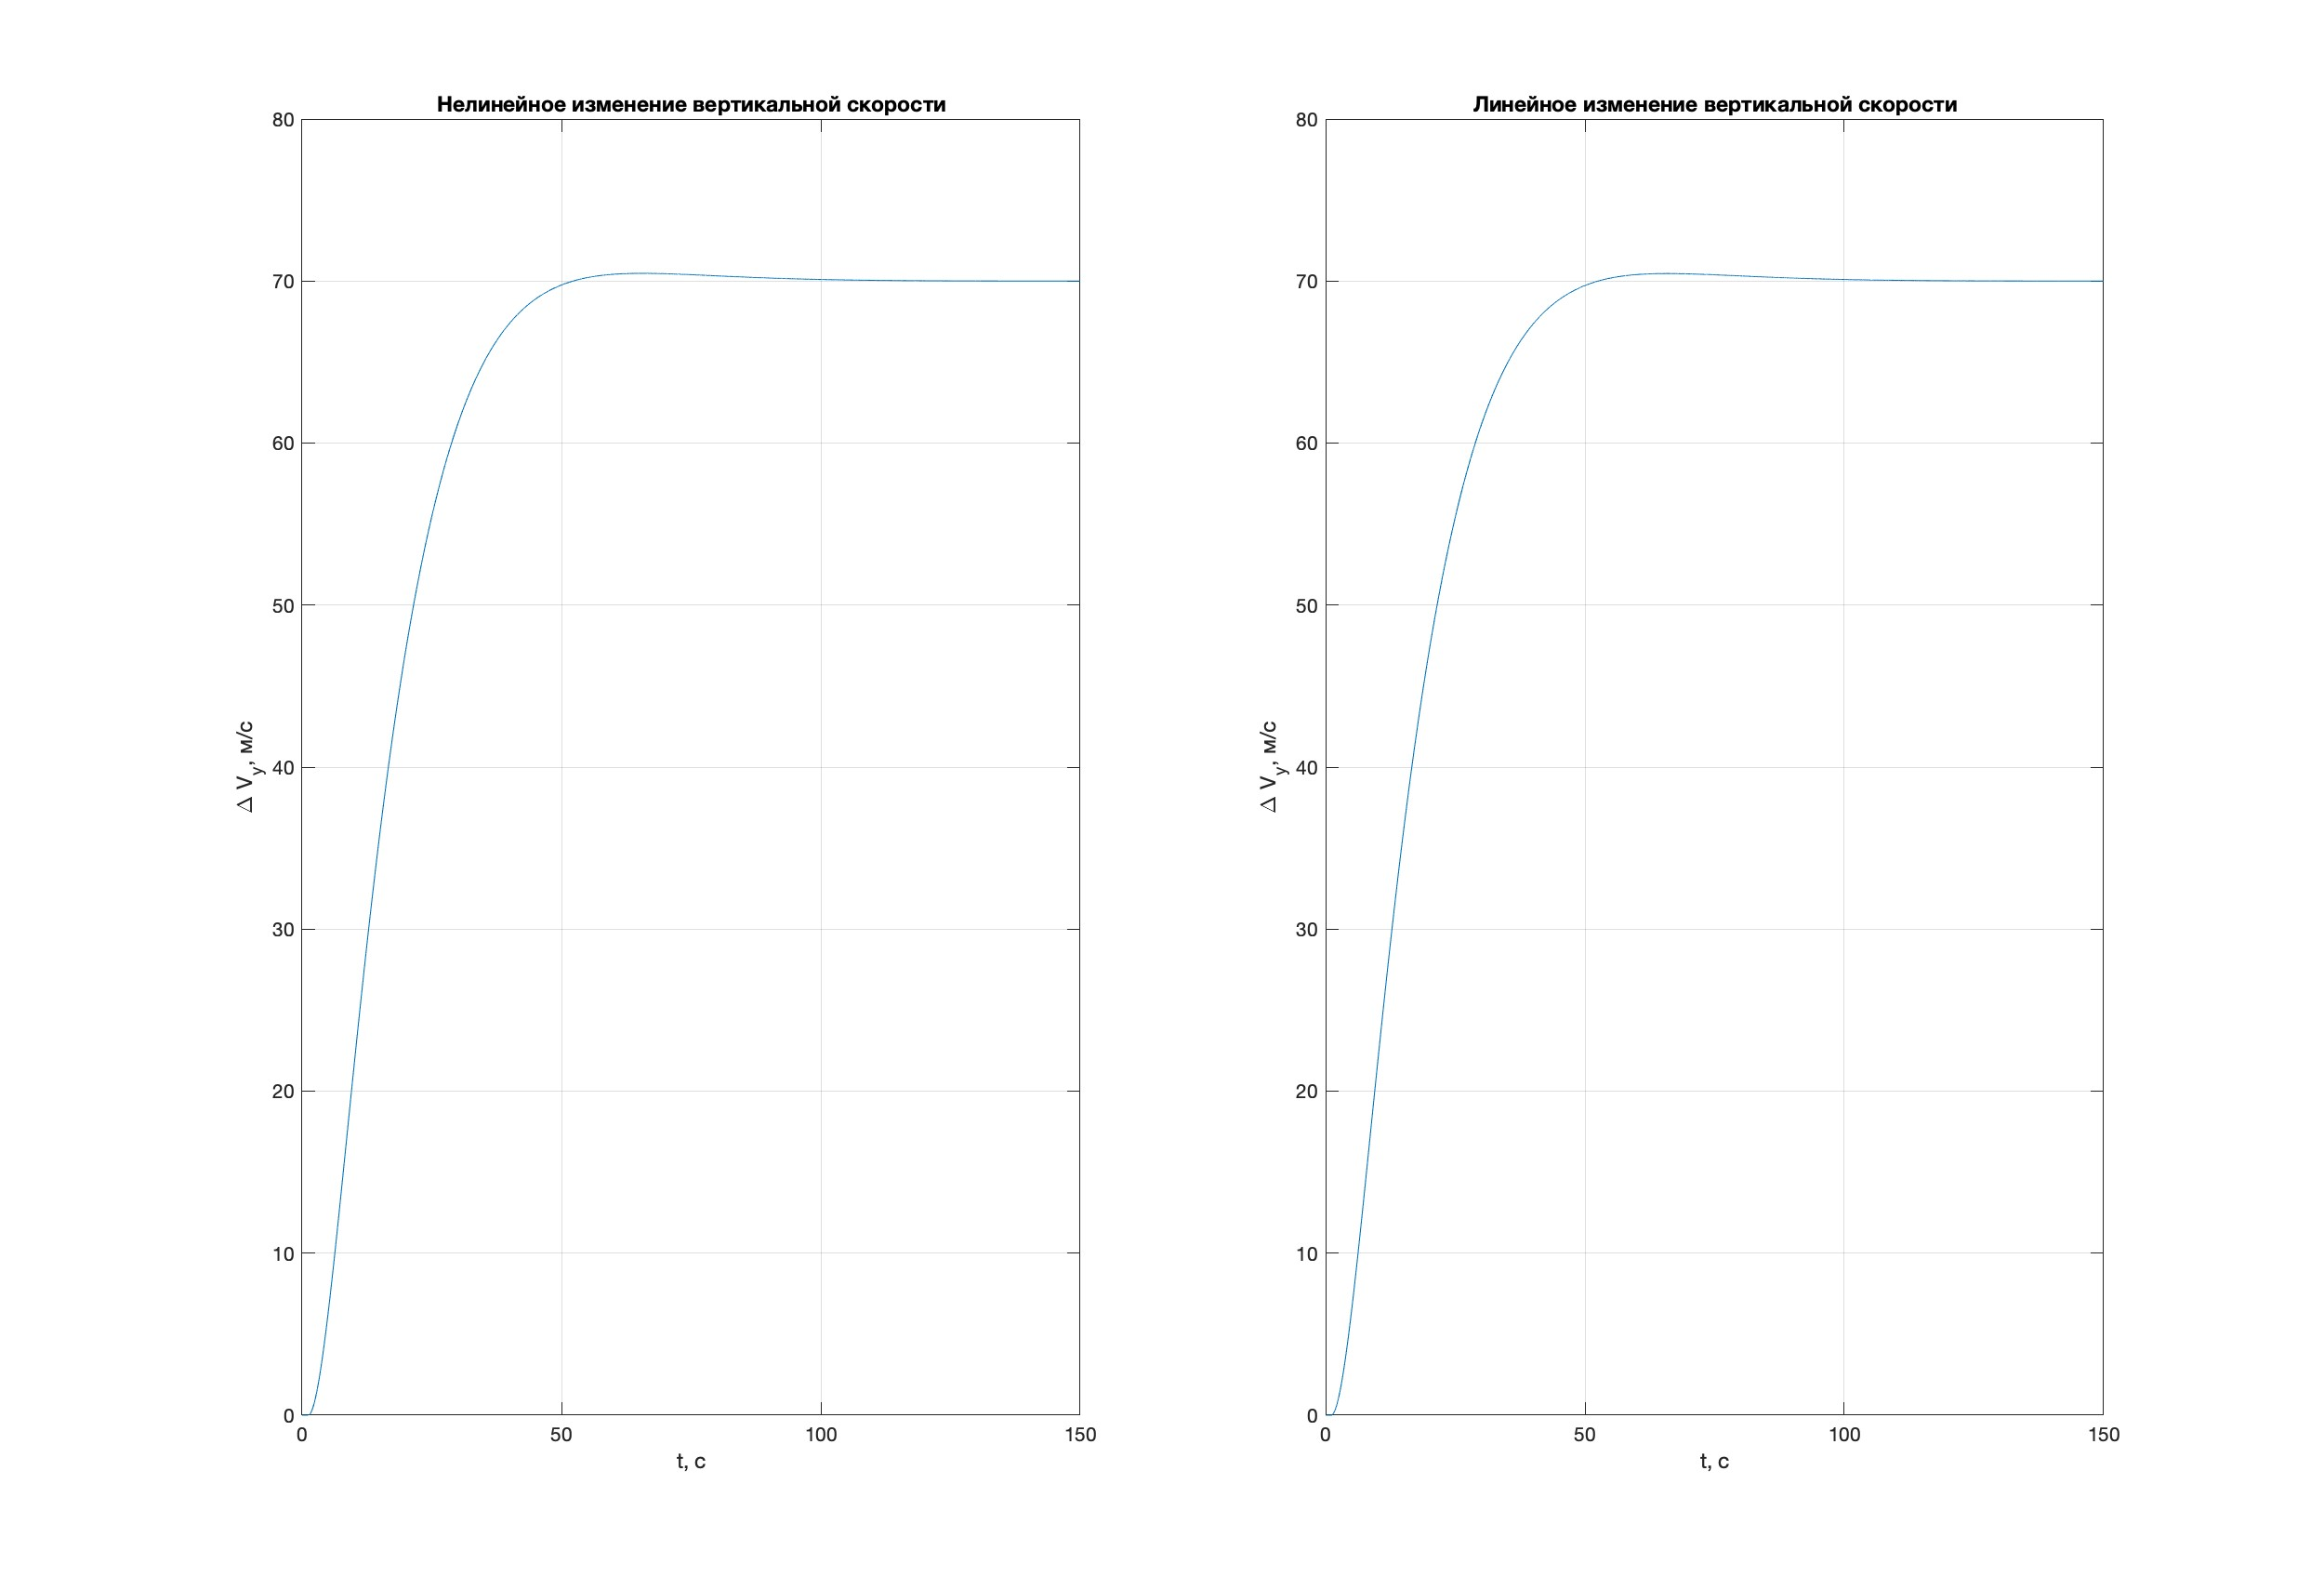
\includegraphics[width=\linewidth]{Оглавление/Part2/Sactions/Content/NotLinFig/Vy.jpg}}
    \caption{Выходной сигнал системы стабилизации вертикальной скорости самолета}
    \label{fig:Входной сигнал системы стабилизации вертикальной скорости}
\end{figure}

%__________________________________________________________________________________________


\begin{center}
    \subsubsubsection{Сравнительный анализ}
\end{center}

Изучив рис.\ref{fig:Отклонения элевонов для стабилизации угла скольжения} можно сделать следующие выводы:
\begin{enumerate}
    \item При введении ограничений на скорость изменения выходного сигнала скорость не превышает 30 град/с что приемлемо, также при введении ограничений на максимальную амплитуду входного и выходного сигналов привод отрабатывает сигнал немного дольше чем без ограничений, «колебательность» сигнала остается одинаковой и в линейном и нелинейном случае.
    \item Также введение ограничений расширяют диапазон заданных значений входного сигнала, то есть при вводе большого значения входного сигнала системы, выходной сигнал привода не превысит значений, указанных в ограничителях, следовательно, при работе системы не произойдет каких-либо неполадок. 
\end{enumerate}
Изучив рис.\ref{fig:Изменение угловой скорости тангажа в процессе стабилизации вертикальной скорости}-\ref{fig:Входной сигнал системы стабилизации вертикальной скорости} можно сделать следующие выводы:

\begin{enumerate}
    \item В линейном и нелинейном случае самолет достигает установившегося значения вертикальной скорости практически за одно и тоже время. 
    \item И в линейной и нелинейной системе вертикальная скорость в конце переходного процесса не равна заданному значению, это связанно с тем, что имеет место быть статическая ошибка. 
\end{enumerate}